\documentclass[12pt,a4paper]{article}

\usepackage[T2A]{fontenc}
\usepackage[utf8]{inputenc}
\usepackage[russian]{babel}
\usepackage{amsmath,amssymb}
\usepackage{geometry}
\usepackage{graphicx}
\usepackage{float}
\usepackage{booktabs}
\usepackage{array}
\usepackage{longtable}
\usepackage{caption}
\usepackage{pdflscape}
\usepackage{hyperref}

\geometry{margin=2.1cm}

\title{Реализация метода нагруженных функций}
\author{}
\date{июнь 2026}

\begin{document}
\maketitle

\section*{Постановка}
Рассматривается задача
\[
J(u)\to \inf,\qquad
u\in U=\{u\in E^1:\ u\in U_0,\ g(u)\le 0\}.
\]
Для каждого варианта из упражнения 1, пункты а), б), г), д), были рассмотрены все предложенные функции \(g(u)\) и все предложенные множества \(U_0\). Например, для пункта а) это \(5\cdot 3=15\) постановок.

Использованы две функции нагружения:
\[
\Phi_{13}(u,t)=L\max\{J(u)-t,0\}+MP(u),
\qquad
\Phi_{32}(u,t)=L|J(u)-t|+MP(u),
\]
где
\[
P(u)=\max\{g(u),0\},\qquad L=1,\quad M=20.
\]
Для каждой постановки численно строилась функция
\[
\rho(t)=\inf_{u\in U_0}\Phi(u,t)
\]
и искался минимальный корень уравнения \(\rho(t)=0\).

\section*{Обработка ограничения \(U_0\)}
Множество \(U_0\) использовалось только как область внутренней минимизации по \(u\). В штраф \(P(u)\) включалось только ограничение \(g(u)\le 0\). Поэтому, если один из концов \(U_0\) равен \(+\infty\) или \(-\infty\), он не превращался в дополнительное искусственное ограничение.

Для численного сеточного поиска неограниченные множества \(U_0\) временно усекались конечным расчётным окном. Это усечение использовалось только для вычислений и построения графиков; в таблице отдельно отмечены случаи пустого допустимого множества и случаи, где инфимум не достигается.

\section*{Варианты}
\begin{itemize}
    \item а) \(J(u)=\arctan u\);
    \item б) \(J(u)=u\sin u\);
    \item г) \(J(u)=1\) при \(u\le 1\), \(J(u)=u^{-1}\) при \(u>1\);
    \item д) \(J(u)=1\).
\end{itemize}
Полный перебор вариантов \(g(u)\) и \(U_0\) приведён в таблице результатов.

\section*{Итоговые результаты}
\begin{landscape}
\scriptsize
\setlength{\tabcolsep}{3pt}
\begin{longtable}{c c p{3.2cm} p{2.7cm} p{2.7cm} c c c c c}
\caption{Результаты для всех вариантов $g(u)$ и $X_0$. Если $U=\varnothing$, условие $t_*=J_*$ не проверяется.}\\
\toprule
№ & п. & $g(u)$ & $X_0$ & аналитически & $x_{13}$ & $t_{13}$ & $x_{32}$ & $t_{32}$ & рис. \\
\midrule
\endfirsthead
\toprule
№ & п. & $g(u)$ & $X_0$ & аналитически & $x_{13}$ & $t_{13}$ & $x_{32}$ & $t_{32}$ & рис. \\
\midrule
\endhead
1 & а & $u^2-4$ & $\{u\in E^1:\ u\geq 1\}$ & $J_*=0.7854$; достигается & 1.0000 & 0.7853 & 1.0000 & 0.7853 & 1 \\
2 & а & $u^2-4$ & $\{u\in E^1:\ u\geq 0\}$ & $J_*=0.0000$; достигается & 0.0000 & -0.0001 & 0.0000 & -0.0001 & 2 \\
3 & а & $u^2-4$ & $E^1$ & $J_*=-1.1071$; достигается & -2.0000 & -1.1072 & -1.9520 & -1.0975 & 3 \\
4 & а & $(u^2-4)(u^4+1)^{-1}$ & $\{u\in E^1:\ u\geq 1\}$ & $J_*=0.7854$; достигается & 1.0000 & 0.7853 & 1.0000 & 0.7853 & 4 \\
5 & а & $(u^2-4)(u^4+1)^{-1}$ & $\{u\in E^1:\ u\geq 0\}$ & $J_*=0.0000$; достигается & 0.0000 & -0.0001 & 0.0000 & -0.0001 & 5 \\
6 & а & $(u^2-4)(u^4+1)^{-1}$ & $E^1$ & $J_*=-1.1071$; достигается & -2.0000 & -1.1072 & -1.9520 & -1.0975 & 6 \\
7 & а & $u$ & $\{u\in E^1:\ u\geq 1\}$ & $J_*=-$; $U=\varnothing$ & 1.0000 & \text{нет} & 1.0000 & \text{нет} & 7 \\
8 & а & $u$ & $\{u\in E^1:\ u\geq 0\}$ & $J_*=0.0000$; достигается & 0.0000 & -0.0001 & 0.0000 & -0.0001 & 8 \\
9 & а & $u$ & $E^1$ & $J_*=-1.5708$; inf не достигается & -20.0000 & -1.5209 & -20.0000 & -1.5209 & 9 \\
10 & а & $u(u^2+1)^{-1}$ & $\{u\in E^1:\ u\geq 1\}$ & $J_*=-$; $U=\varnothing$ & 4.0000 & \text{нет} & 4.0000 & \text{нет} & 10 \\
11 & а & $u(u^2+1)^{-1}$ & $\{u\in E^1:\ u\geq 0\}$ & $J_*=0.0000$; достигается & 0.0000 & -0.0001 & 0.0000 & -0.0001 & 11 \\
12 & а & $u(u^2+1)^{-1}$ & $E^1$ & $J_*=-1.5708$; inf не достигается & -20.0000 & -1.5209 & -20.0000 & -1.5209 & 12 \\
13 & а & $u^2$ & $\{u\in E^1:\ u\geq 1\}$ & $J_*=-$; $U=\varnothing$ & 1.0000 & \text{нет} & 1.0000 & \text{нет} & 13 \\
14 & а & $u^2$ & $\{u\in E^1:\ u\geq 0\}$ & $J_*=0.0000$; достигается & 0.0000 & -0.0001 & 0.0000 & -0.0001 & 14 \\
15 & а & $u^2$ & $E^1$ & $J_*=0.0000$; достигается & 0.0000 & -0.0001 & 0.0000 & -0.0001 & 15 \\
16 & б & $u^2-1$ & $\{u\in E^1:\ u\geq 0\}$ & $J_*=0.0000$; достигается & 0.0000 & -0.0001 & 0.0000 & -0.0001 & 16 \\
17 & б & $(u^2-1)(u^4+1)^{-1}$ & $\{u\in E^1:\ u\geq 0\}$ & $J_*=0.0000$; достигается & 0.0000 & -0.0001 & 0.0000 & -0.0001 & 17 \\
18 & б & $(u^2-1)e^{-u^2}$ & $\{u\in E^1:\ u\geq 0\}$ & $J_*=0.0000$; достигается & 4.0000 & -3.0273 & 3.9928 & -3.0030 & 18 \\
19 & г & $u-1$ & $\{u\in E^1:\ u\geq 0\}$ & $J_*=1.0000$; неединственный минимум & 0.0000 & 0.9999 & 0.0000 & 0.9999 & 19 \\
20 & г & $u-1$ & $E^1$ & $J_*=1.0000$; неединственный минимум & -8.0000 & 0.9999 & -8.0000 & 0.9999 & 20 \\
21 & г & $(u-2)(u^2+1)^{-1}$ & $\{u\in E^1:\ u\geq 0\}$ & $J_*=0.5000$; достигается & 2.0000 & 0.4999 & 2.0000 & 0.4999 & 21 \\
22 & г & $(u-2)(u^2+1)^{-1}$ & $E^1$ & $J_*=0.5000$; достигается & 2.0000 & 0.4999 & 2.0000 & 0.4999 & 22 \\
23 & г & $e^{-u^2}$ & $\{u\in E^1:\ u\geq 0\}$ & $J_*=-$; $U=\varnothing$ & 8.0000 & 0.1249 & 8.0000 & 0.1249 & 23 \\
24 & г & $e^{-u^2}$ & $E^1$ & $J_*=-$; $U=\varnothing$ & 8.0000 & 0.1249 & 8.0000 & 0.1249 & 24 \\
25 & д & $u$ & $E^1$ & $J_*=1.0000$; неединственный минимум & -8.0000 & 0.9999 & -8.0000 & 0.9999 & 25 \\
26 & д & $u$ & $\{u\in E^1:\ u\geq 0\}$ & $J_*=1.0000$; достигается & 0.0000 & 0.9999 & 0.0000 & 0.9999 & 26 \\
27 & д & $u^2+1$ & $E^1$ & $J_*=-$; $U=\varnothing$ & 0.0000 & \text{нет} & 0.0000 & \text{нет} & 27 \\
28 & д & $u^2+1$ & $\{u\in E^1:\ u\geq 0\}$ & $J_*=-$; $U=\varnothing$ & 0.0000 & \text{нет} & 0.0000 & \text{нет} & 28 \\
29 & д & $e^{-u^2}(u^2+1)$ & $E^1$ & $J_*=-$; $U=\varnothing$ & -8.0000 & 0.9999 & -8.0000 & 0.9999 & 29 \\
30 & д & $e^{-u^2}(u^2+1)$ & $\{u\in E^1:\ u\geq 0\}$ & $J_*=-$; $U=\varnothing$ & 7.3104 & 0.9999 & 7.3104 & 0.9999 & 30 \\
31 & д & $u^2e^{-u^2}$ & $E^1$ & $J_*=1.0000$; достигается & -8.0000 & 0.9999 & -8.0000 & 0.9999 & 31 \\
32 & д & $u^2e^{-u^2}$ & $\{u\in E^1:\ u\geq 0\}$ & $J_*=1.0000$; достигается & 0.0000 & 0.9999 & 0.0000 & 0.9999 & 32 \\
\bottomrule
\end{longtable}
\end{landscape}

\section*{Графики}
Каждый рисунок соответствует одной паре \(g(u),U_0\). Верхний ряд показывает исходную функцию, найденную точку и допустимую область для \(\Phi_{13}\) и \(\Phi_{32}\). Нижний ряд показывает линии уровня соответствующей \(\Phi(u,t)\) и допустимую область.

\begin{figure}[H]
\centering
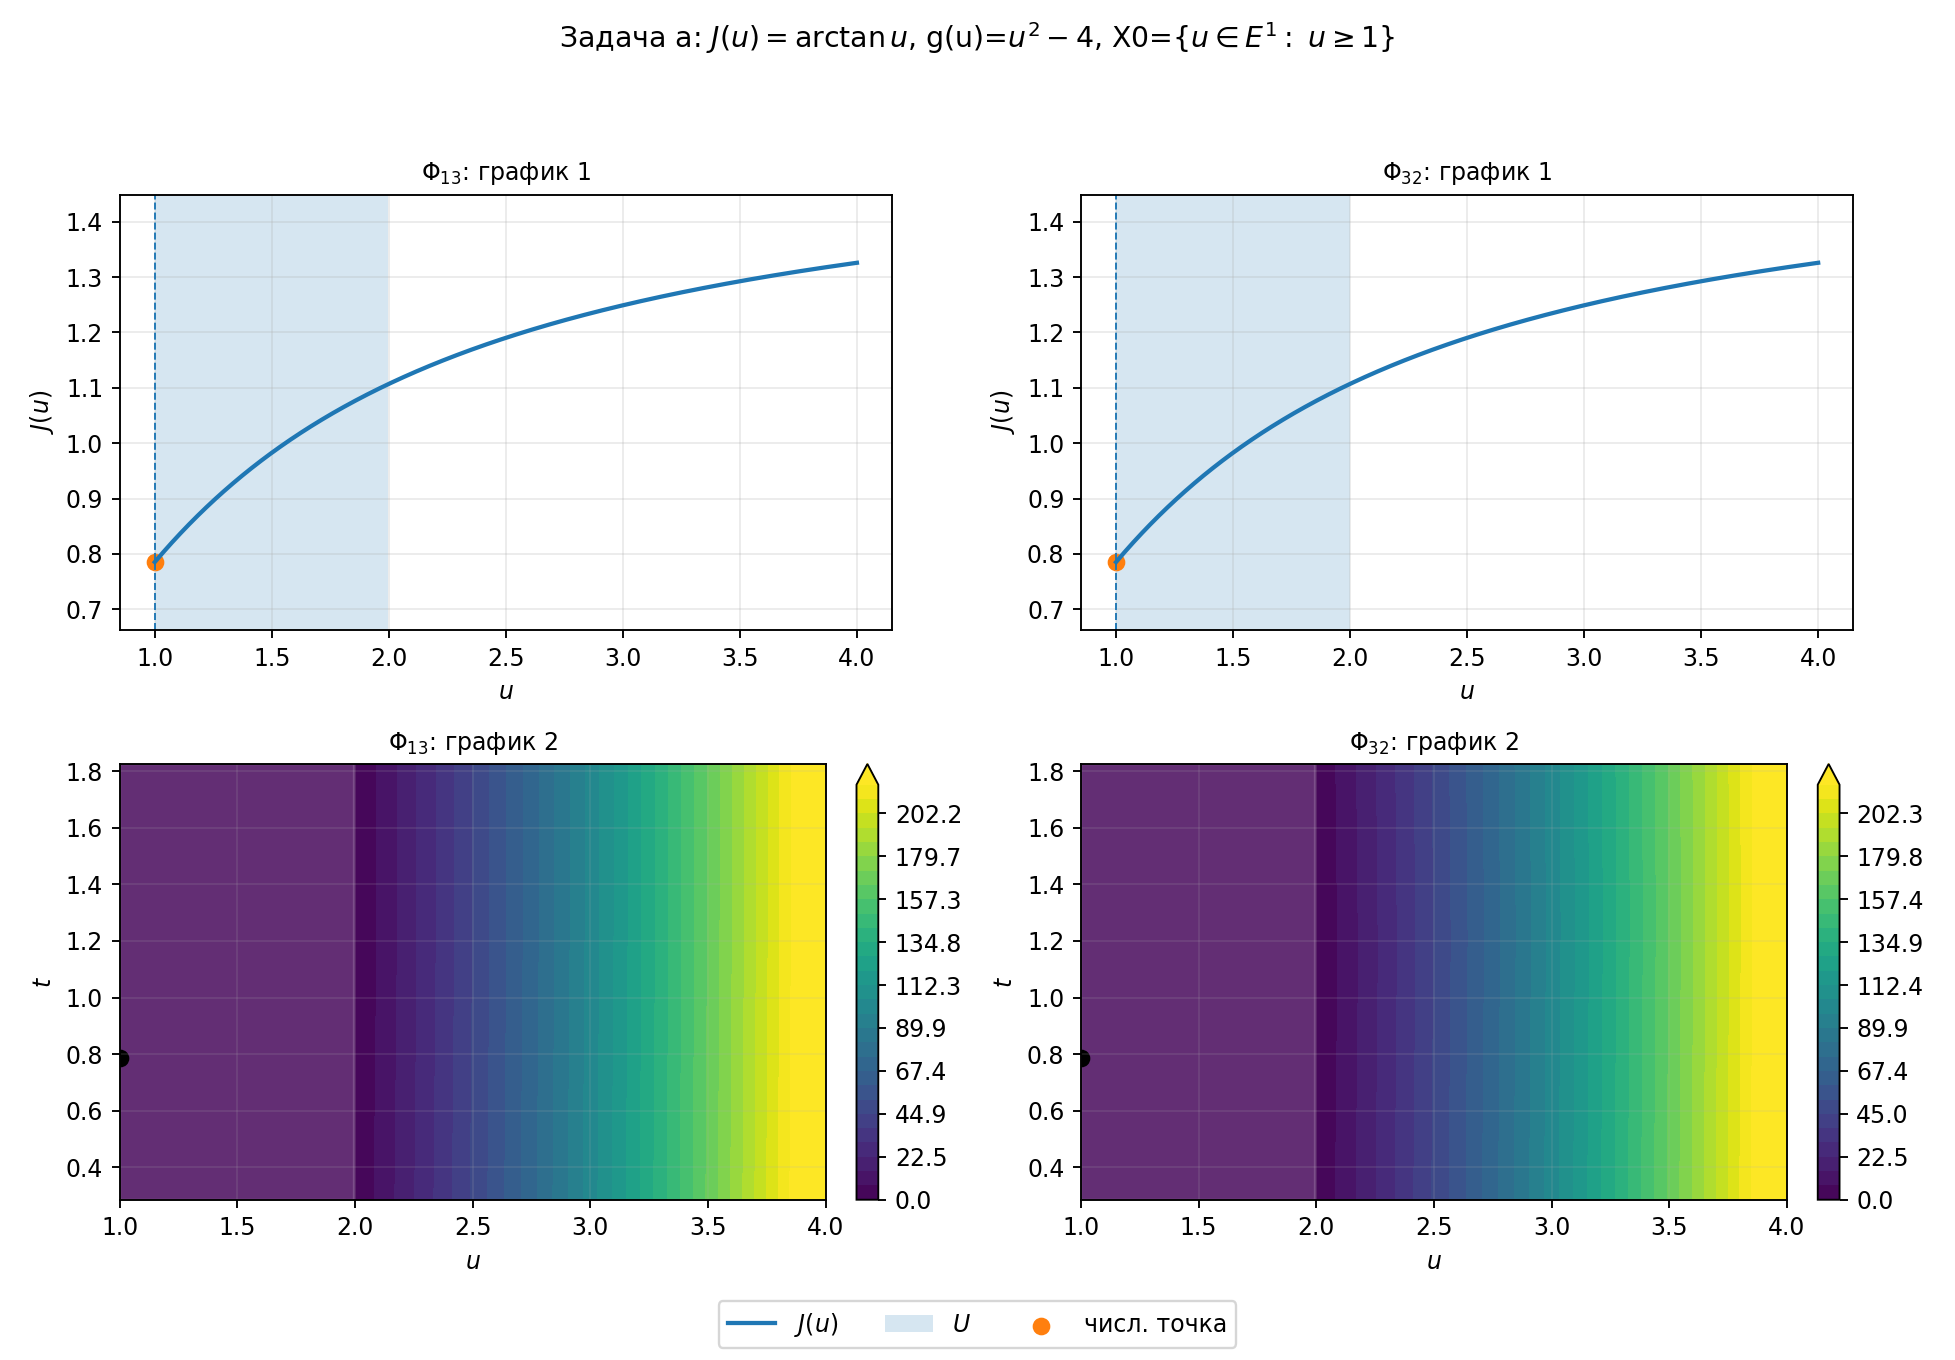
\includegraphics[width=0.96\textwidth]{graphs/a_g1_xge1_overview.png}
\caption{Задача а, вариант g1: $g(u)=u^2-4$, $X_0=\{u\in E^1:\ u\geq 1\}$. Верхний ряд: график 1 для $\Phi_{13}$ и $\Phi_{32}$; нижний ряд: график 2 для $\Phi_{13}$ и $\Phi_{32}$.}
\end{figure}

\begin{figure}[H]
\centering
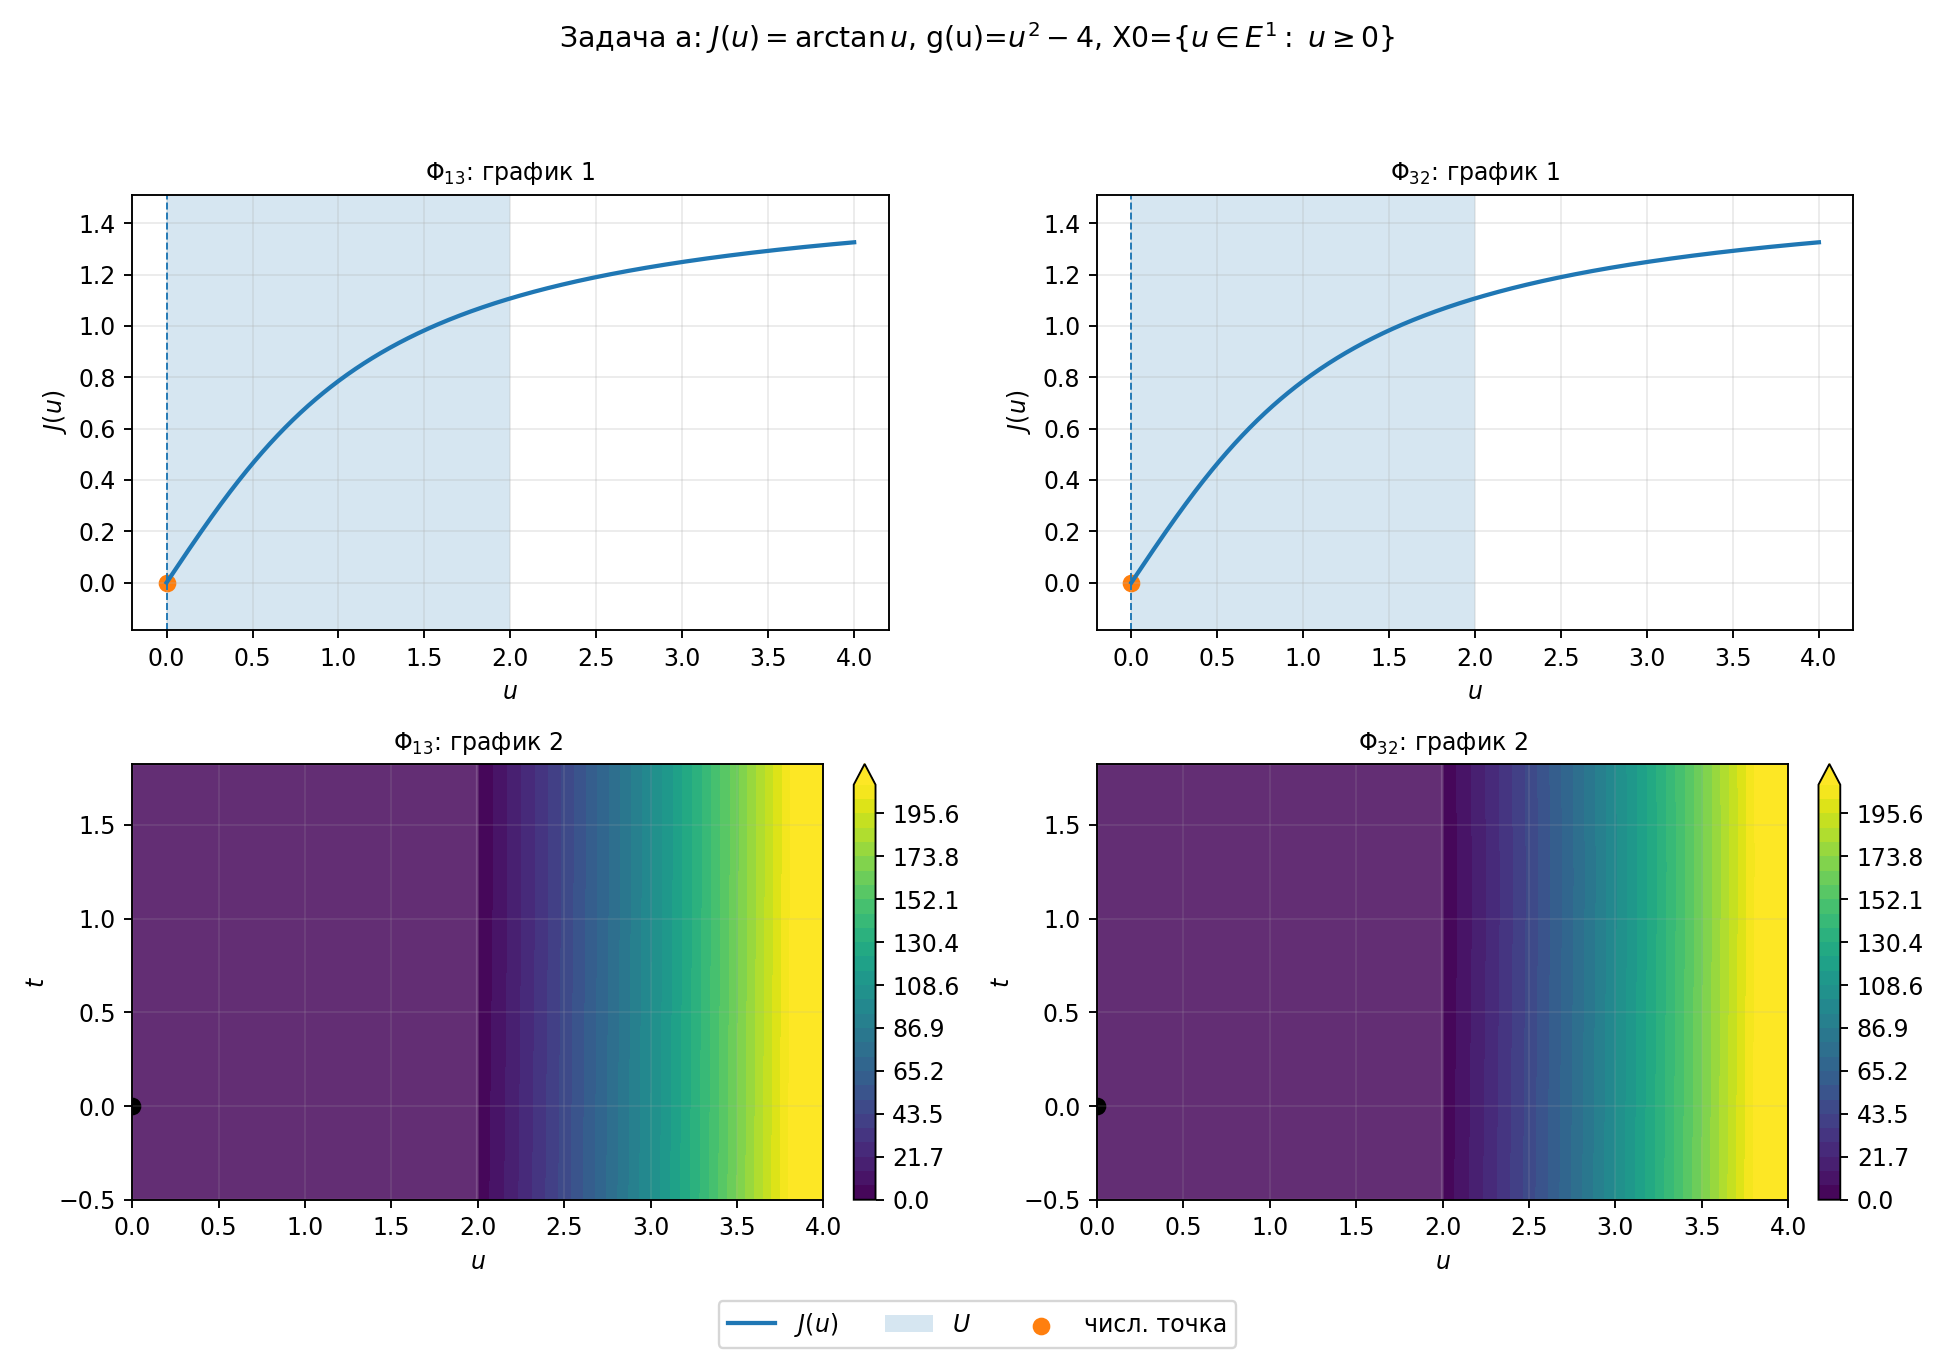
\includegraphics[width=0.96\textwidth]{graphs/a_g1_xge0_overview.png}
\caption{Задача а, вариант g1: $g(u)=u^2-4$, $X_0=\{u\in E^1:\ u\geq 0\}$. Верхний ряд: график 1 для $\Phi_{13}$ и $\Phi_{32}$; нижний ряд: график 2 для $\Phi_{13}$ и $\Phi_{32}$.}
\end{figure}

\begin{figure}[H]
\centering
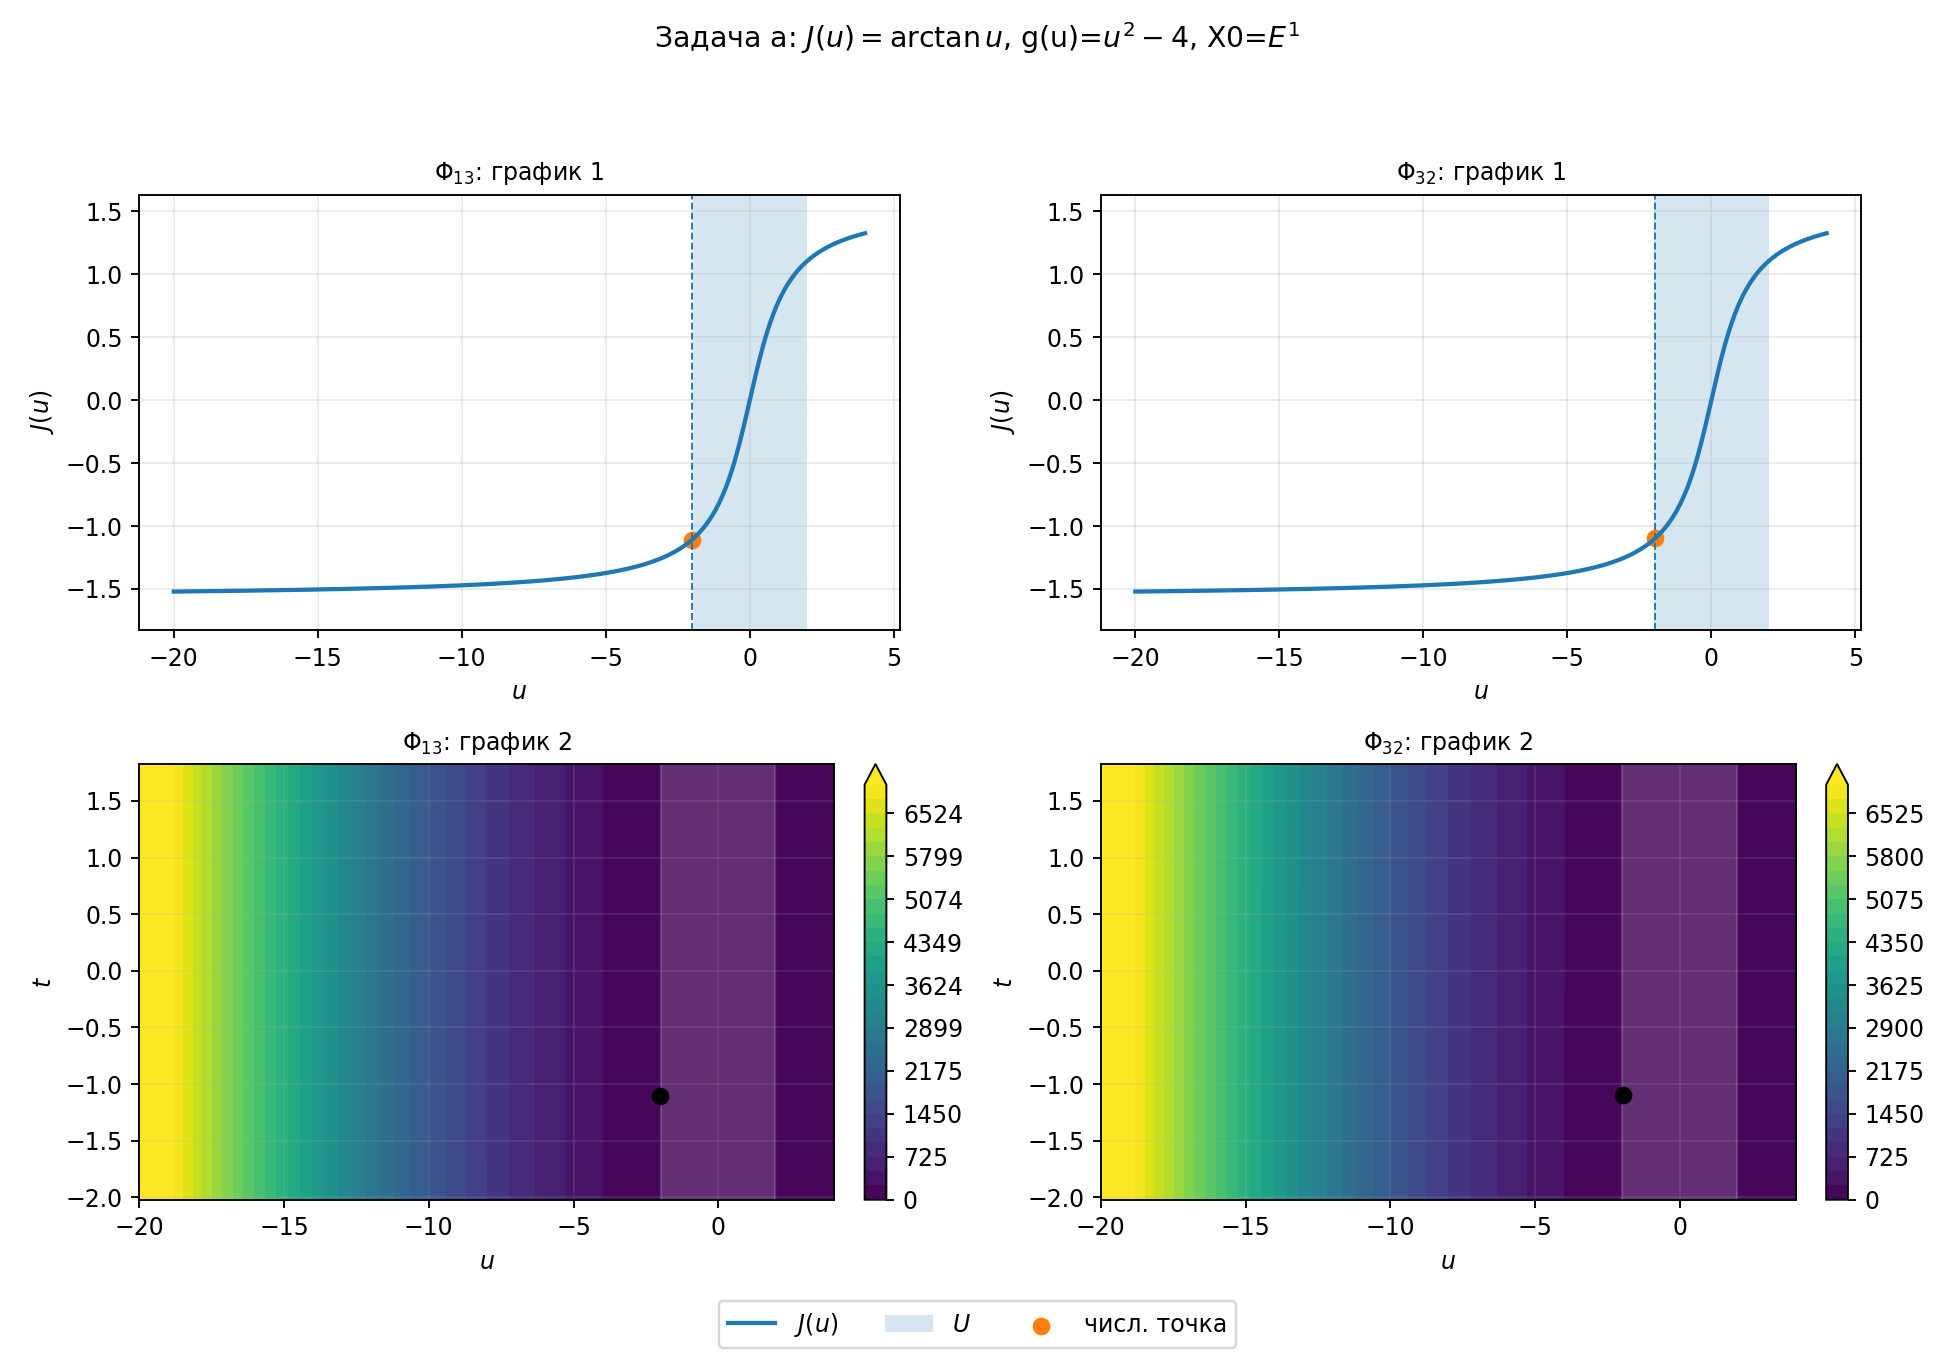
\includegraphics[width=0.96\textwidth]{graphs/a_g1_R_overview.png}
\caption{Задача а, вариант g1: $g(u)=u^2-4$, $X_0=E^1$. Верхний ряд: график 1 для $\Phi_{13}$ и $\Phi_{32}$; нижний ряд: график 2 для $\Phi_{13}$ и $\Phi_{32}$.}
\end{figure}

\begin{figure}[H]
\centering
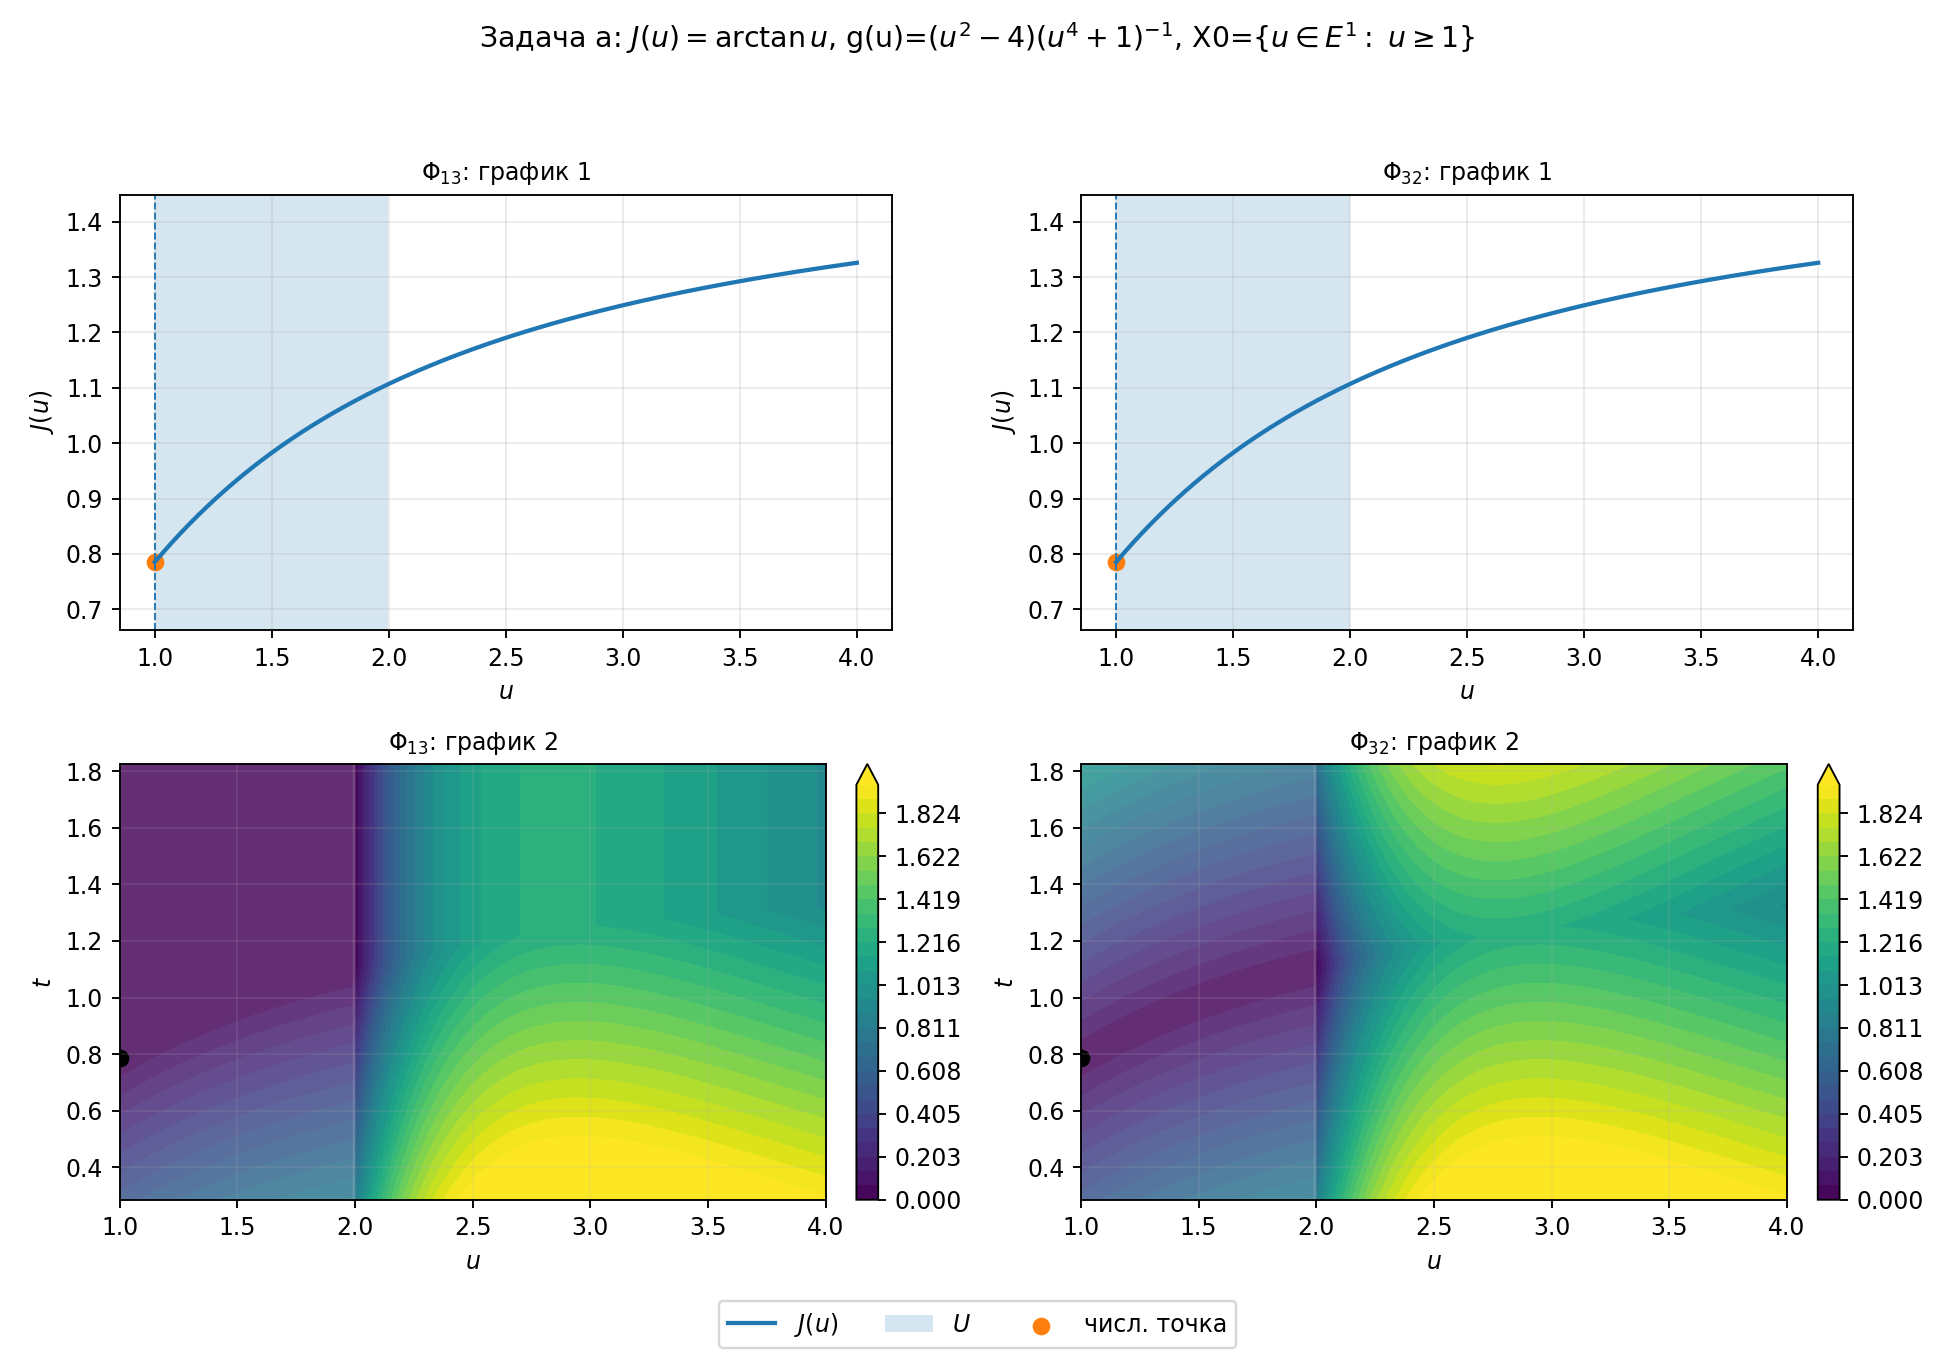
\includegraphics[width=0.96\textwidth]{graphs/a_g2_xge1_overview.png}
\caption{Задача а, вариант g2: $g(u)=(u^2-4)(u^4+1)^{-1}$, $X_0=\{u\in E^1:\ u\geq 1\}$. Верхний ряд: график 1 для $\Phi_{13}$ и $\Phi_{32}$; нижний ряд: график 2 для $\Phi_{13}$ и $\Phi_{32}$.}
\end{figure}

\begin{figure}[H]
\centering
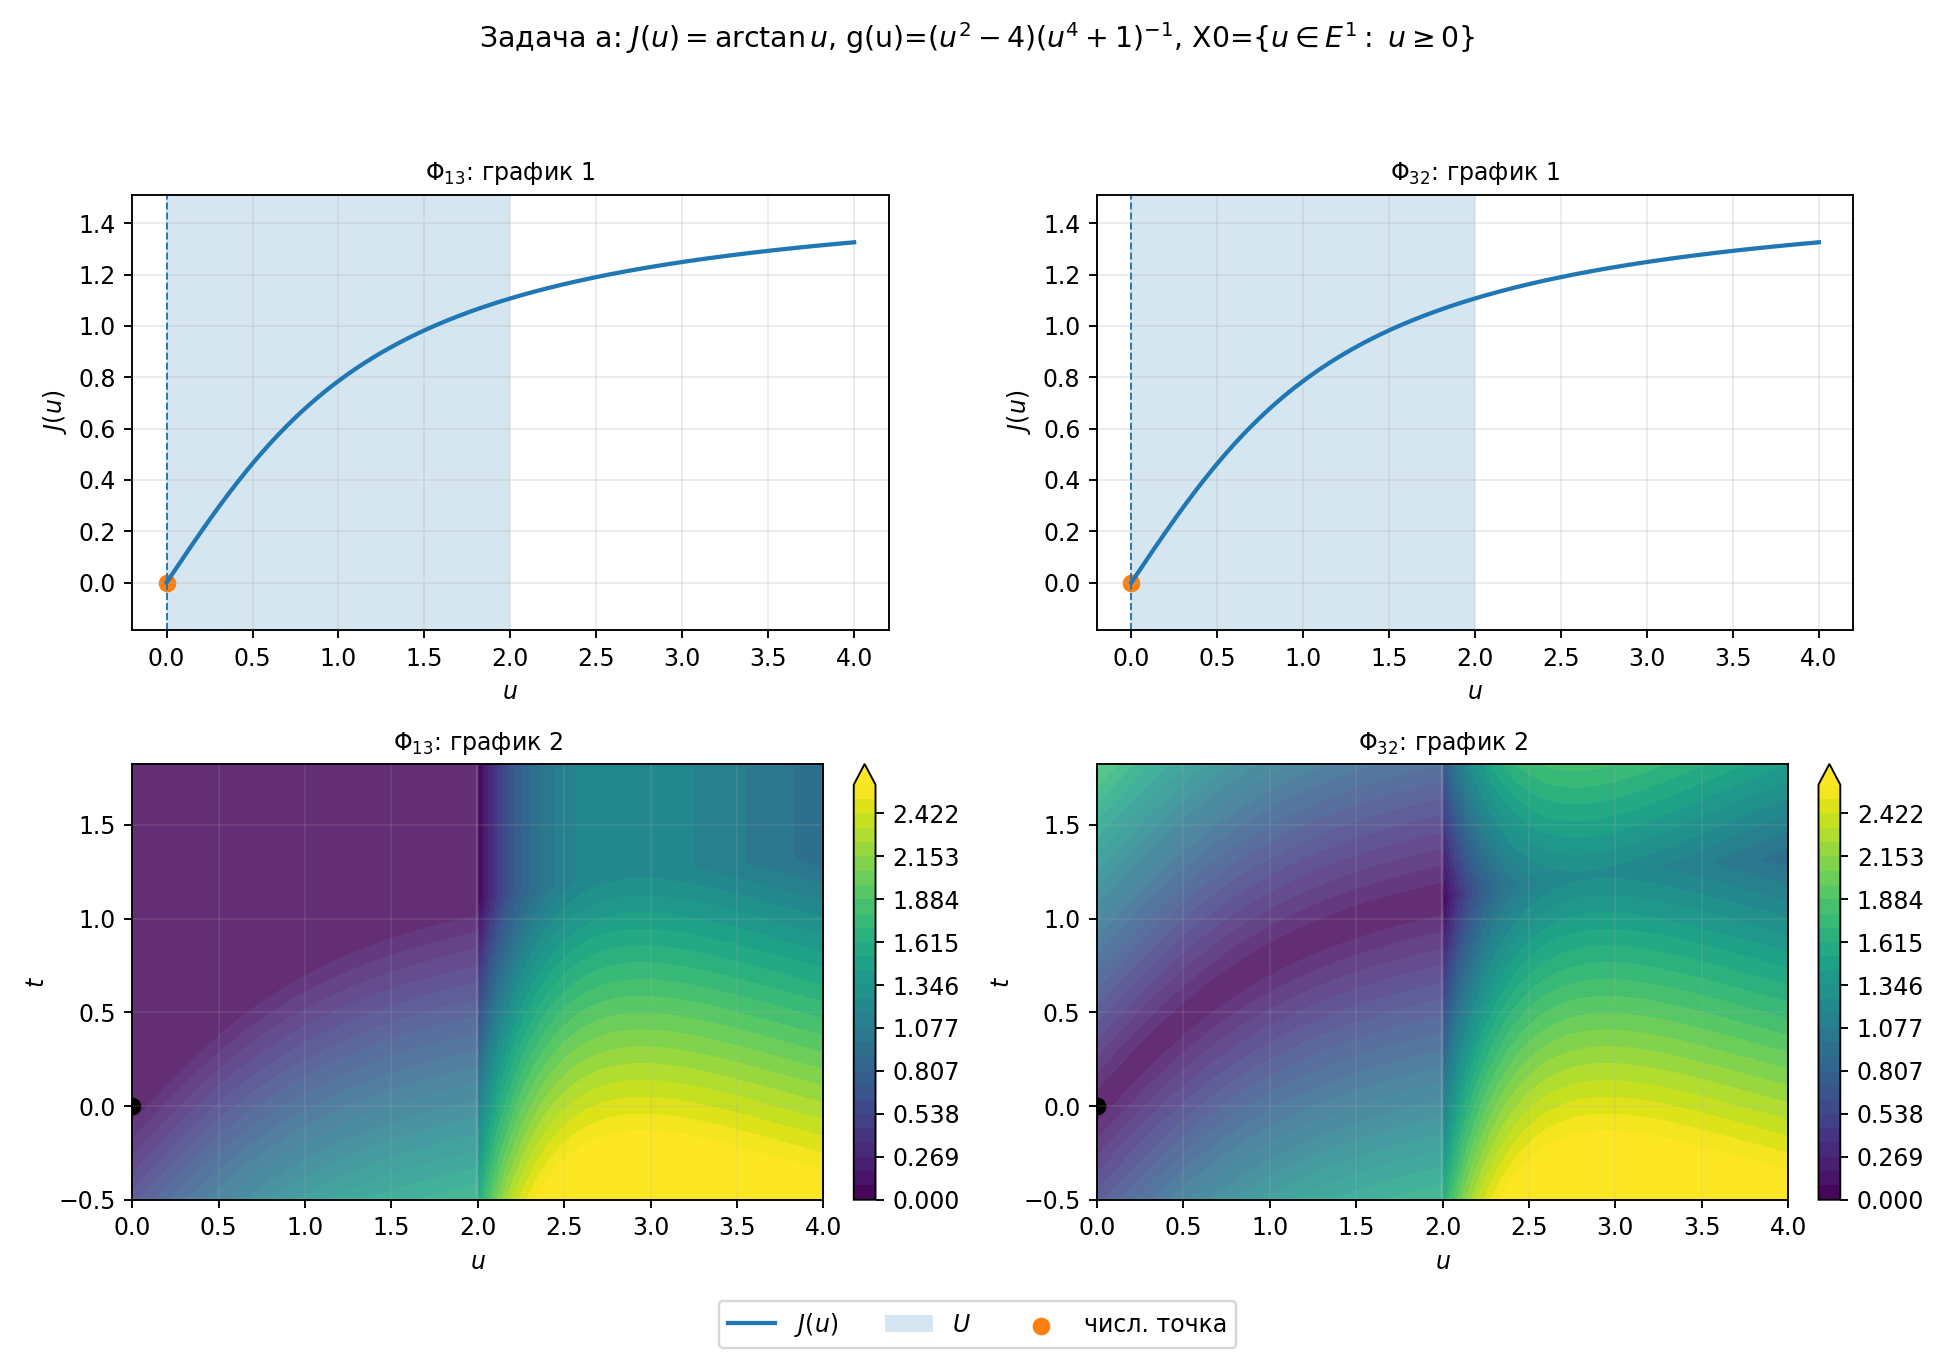
\includegraphics[width=0.96\textwidth]{graphs/a_g2_xge0_overview.png}
\caption{Задача а, вариант g2: $g(u)=(u^2-4)(u^4+1)^{-1}$, $X_0=\{u\in E^1:\ u\geq 0\}$. Верхний ряд: график 1 для $\Phi_{13}$ и $\Phi_{32}$; нижний ряд: график 2 для $\Phi_{13}$ и $\Phi_{32}$.}
\end{figure}

\begin{figure}[H]
\centering
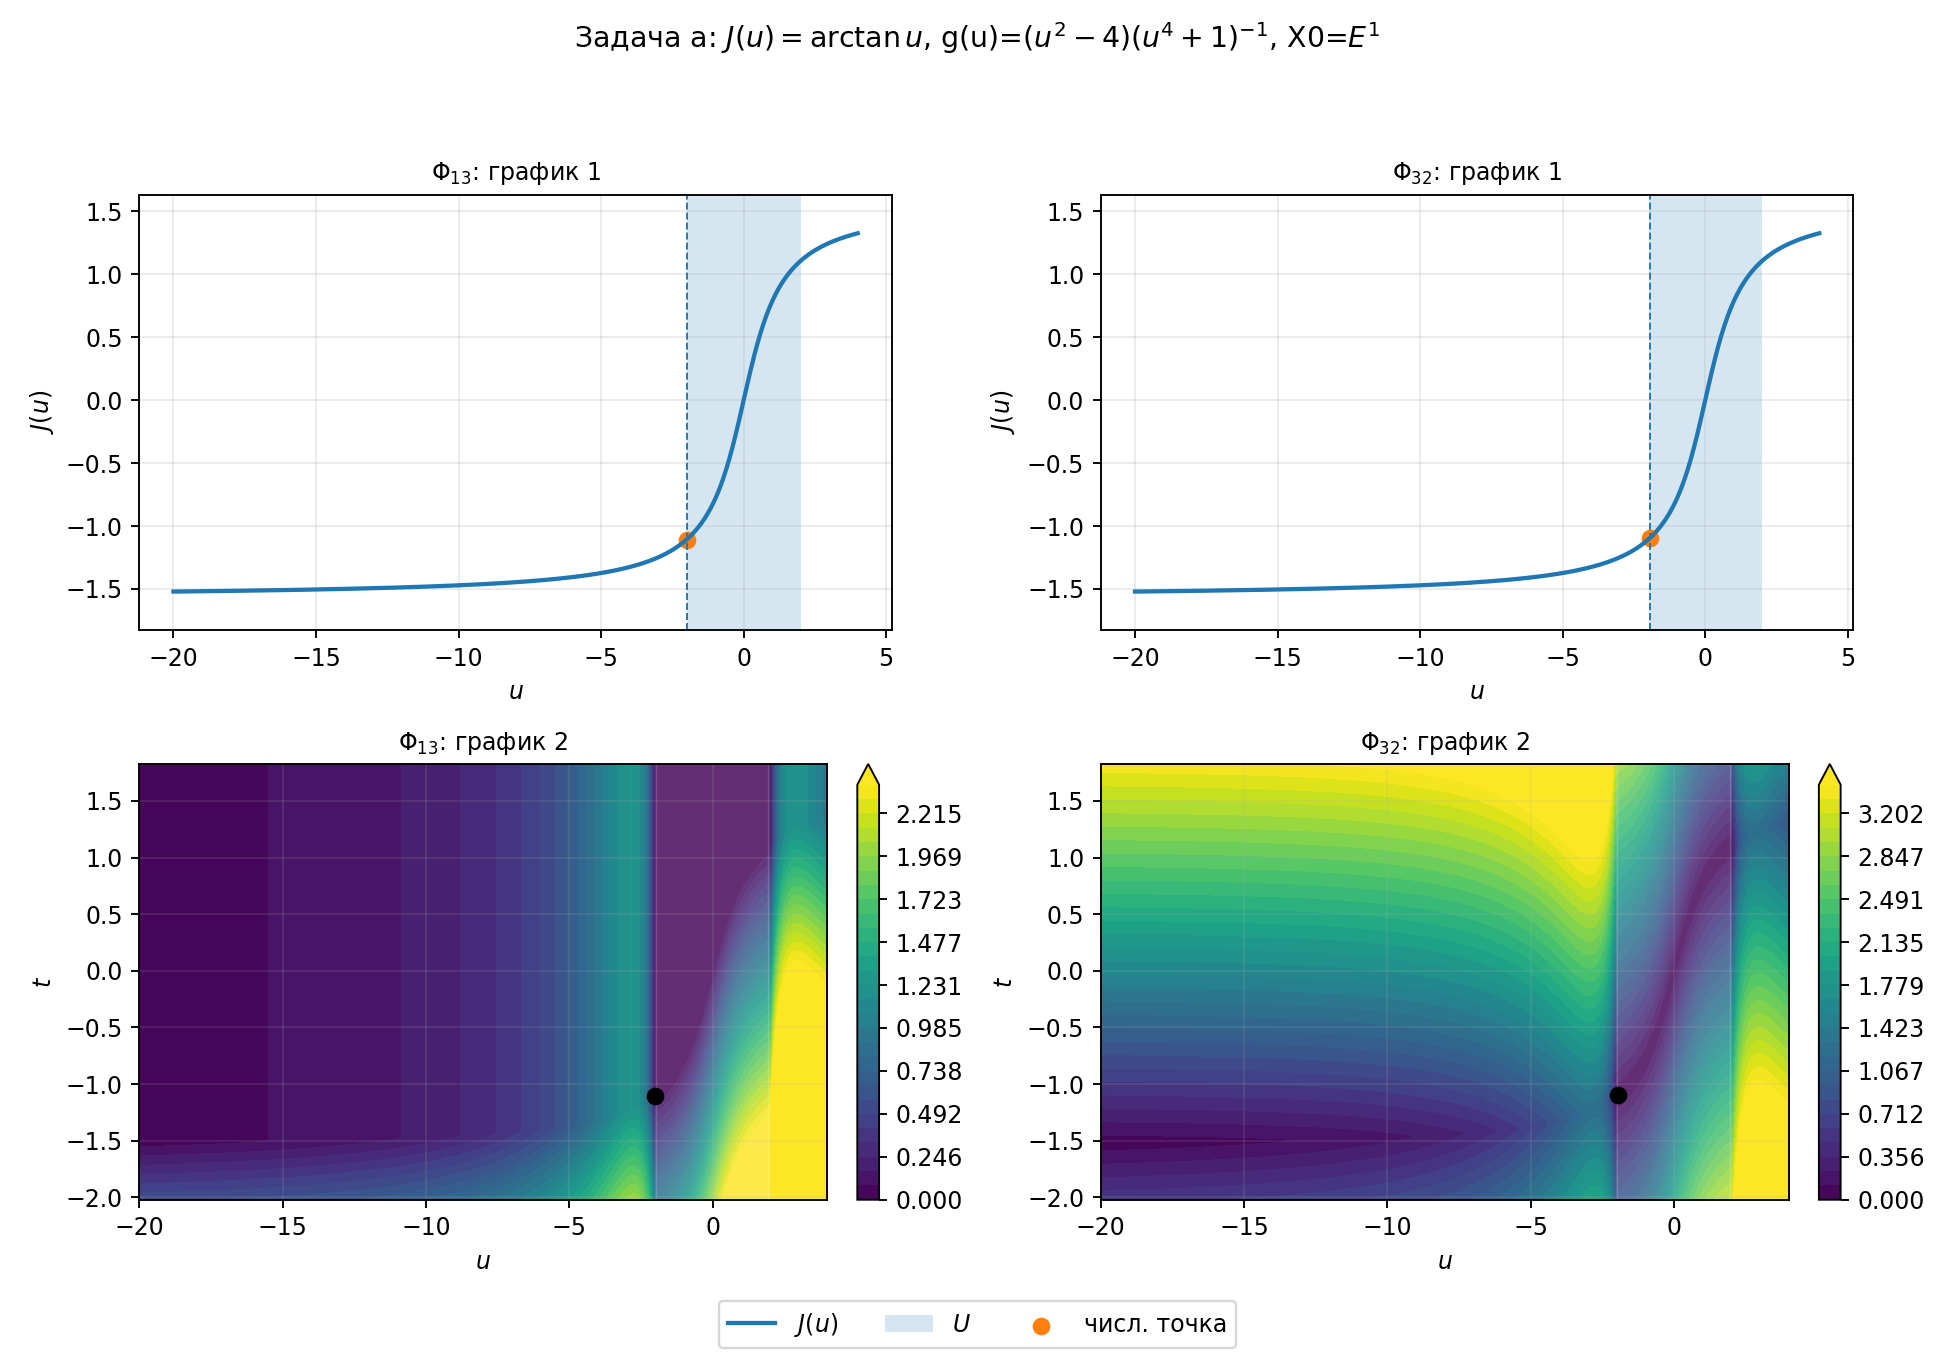
\includegraphics[width=0.96\textwidth]{graphs/a_g2_R_overview.png}
\caption{Задача а, вариант g2: $g(u)=(u^2-4)(u^4+1)^{-1}$, $X_0=E^1$. Верхний ряд: график 1 для $\Phi_{13}$ и $\Phi_{32}$; нижний ряд: график 2 для $\Phi_{13}$ и $\Phi_{32}$.}
\end{figure}

\begin{figure}[H]
\centering
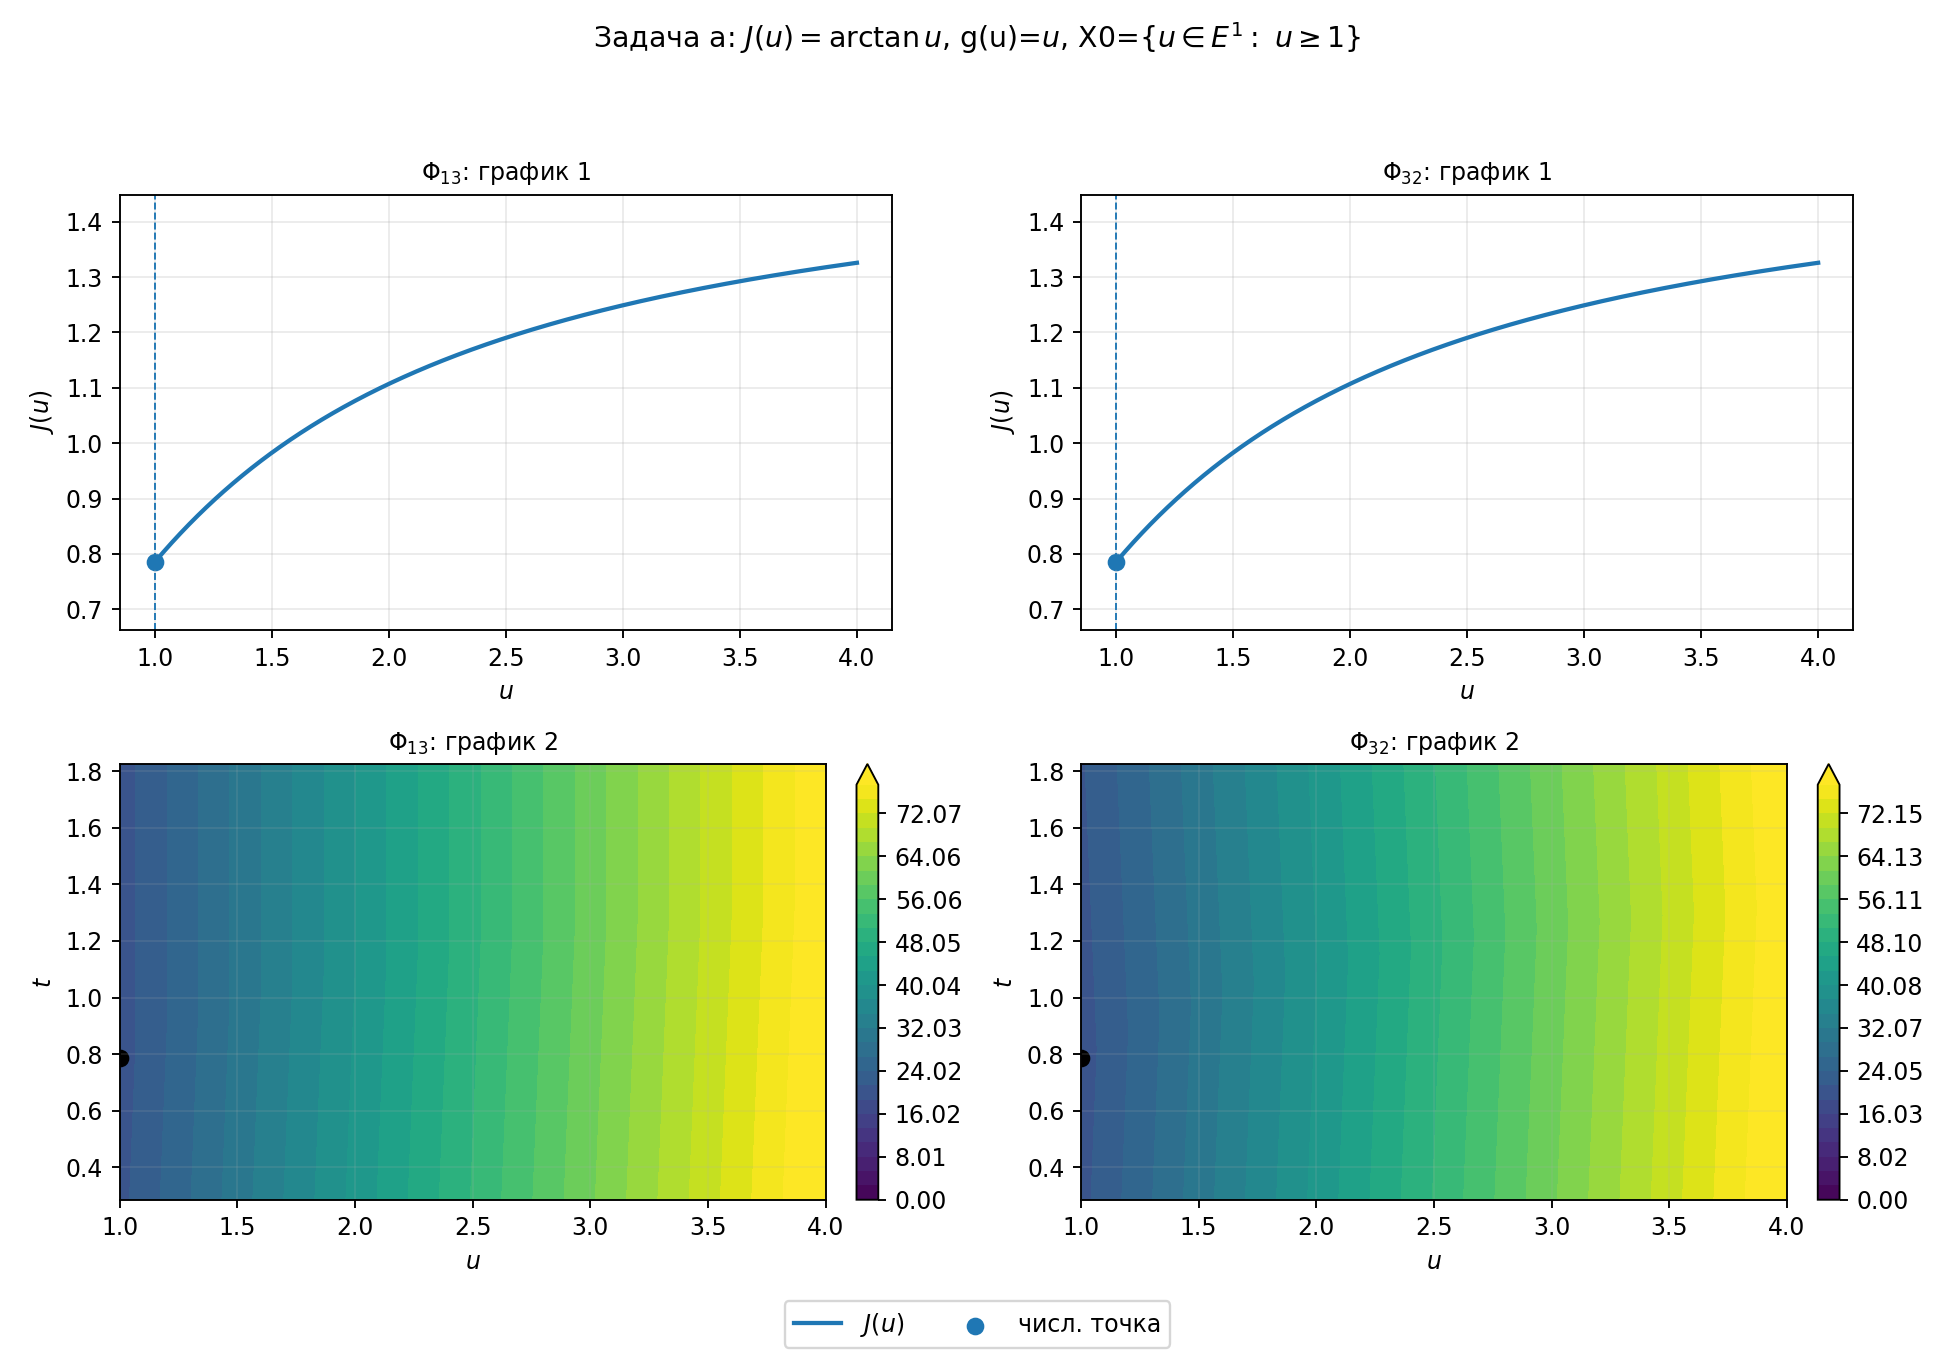
\includegraphics[width=0.96\textwidth]{graphs/a_g3_xge1_overview.png}
\caption{Задача а, вариант g3: $g(u)=u$, $X_0=\{u\in E^1:\ u\geq 1\}$. Верхний ряд: график 1 для $\Phi_{13}$ и $\Phi_{32}$; нижний ряд: график 2 для $\Phi_{13}$ и $\Phi_{32}$.}
\end{figure}

\begin{figure}[H]
\centering
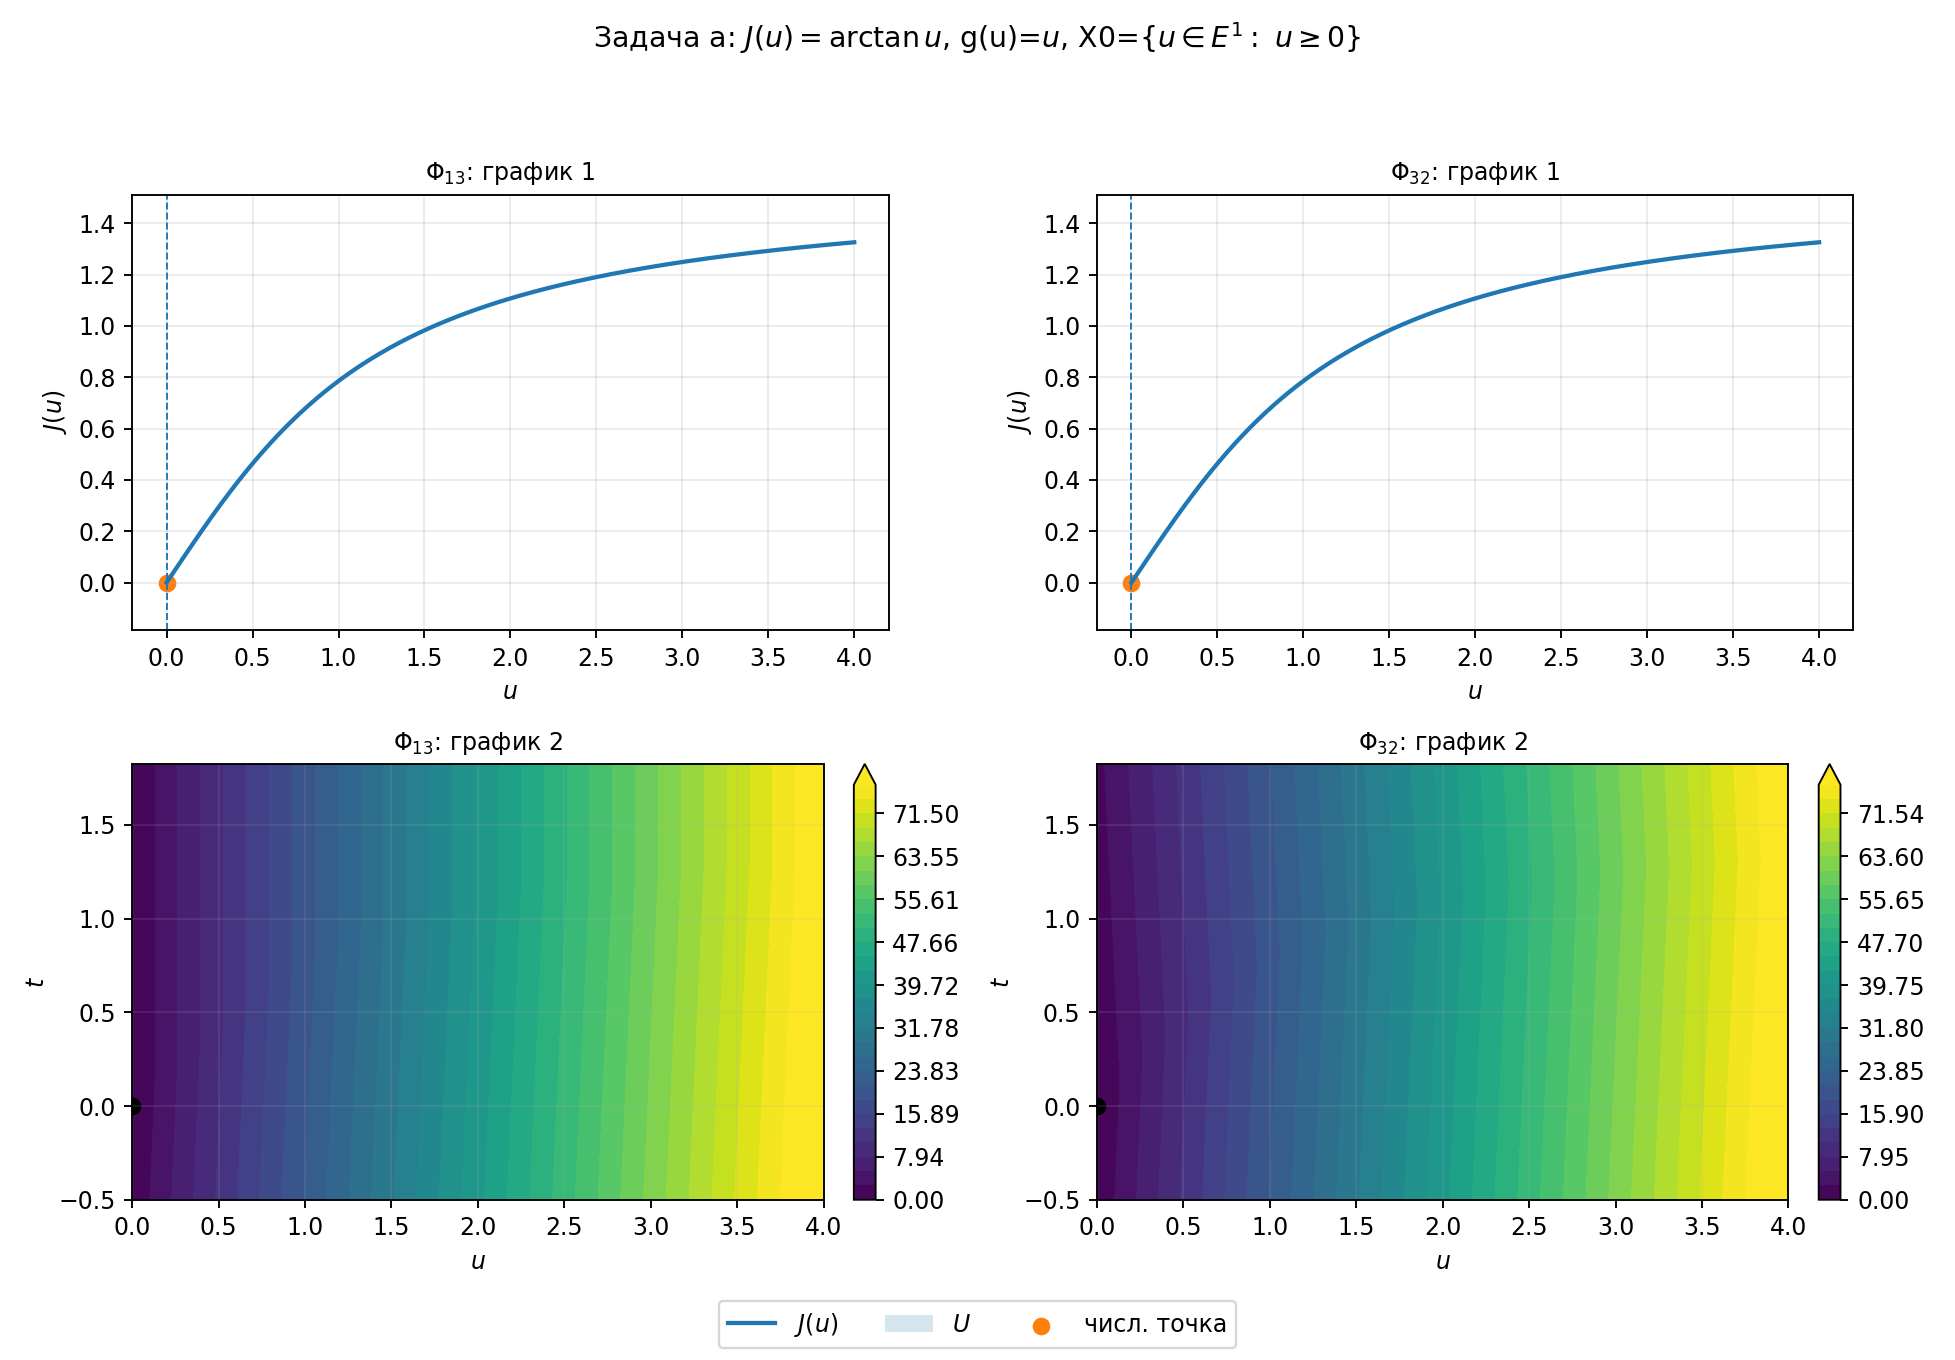
\includegraphics[width=0.96\textwidth]{graphs/a_g3_xge0_overview.png}
\caption{Задача а, вариант g3: $g(u)=u$, $X_0=\{u\in E^1:\ u\geq 0\}$. Верхний ряд: график 1 для $\Phi_{13}$ и $\Phi_{32}$; нижний ряд: график 2 для $\Phi_{13}$ и $\Phi_{32}$.}
\end{figure}

\begin{figure}[H]
\centering
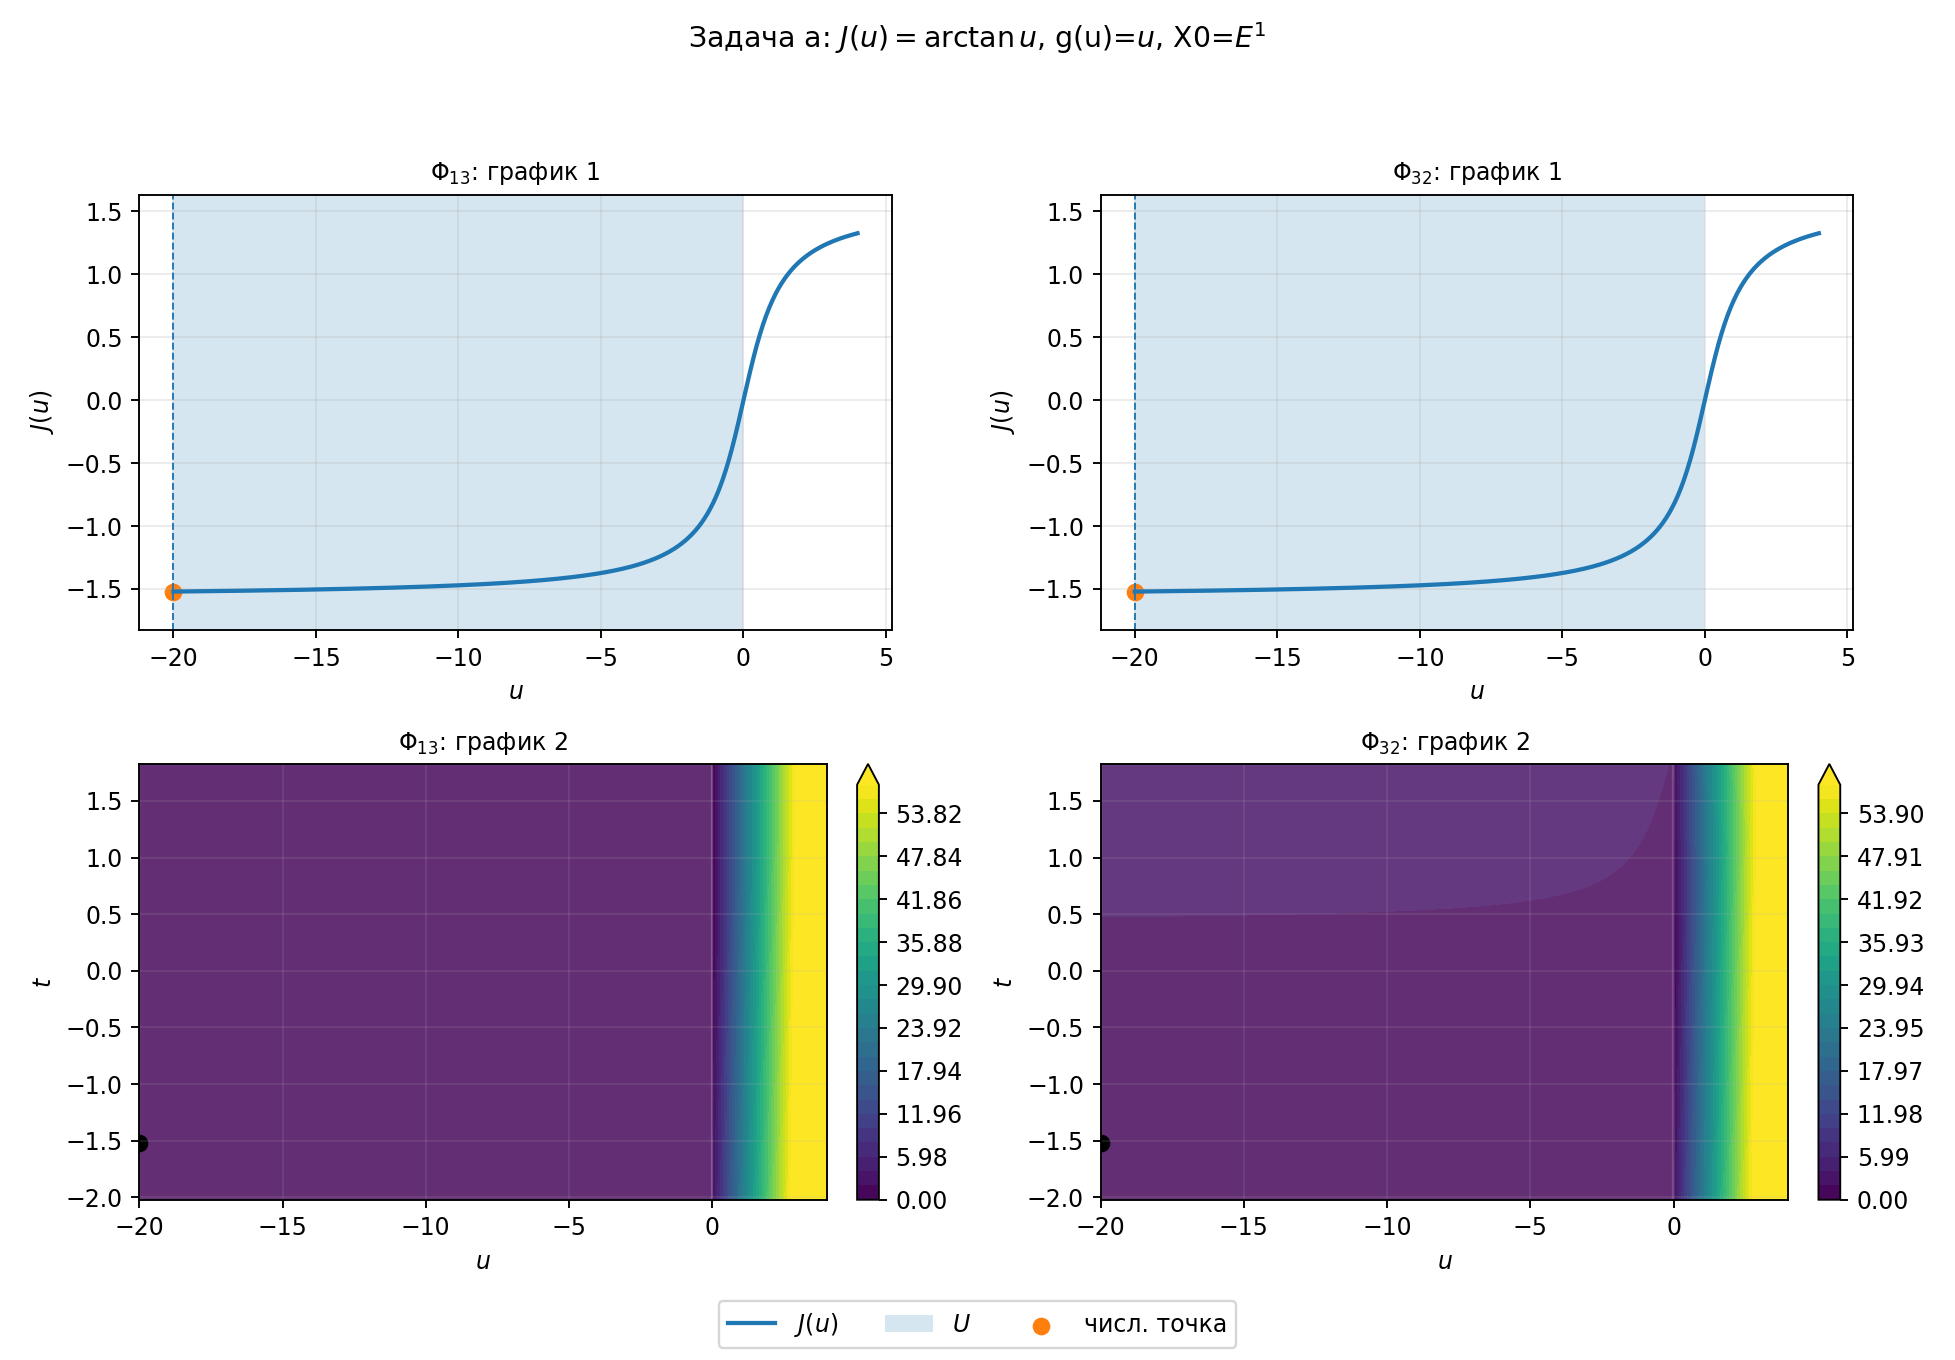
\includegraphics[width=0.96\textwidth]{graphs/a_g3_R_overview.png}
\caption{Задача а, вариант g3: $g(u)=u$, $X_0=E^1$. Верхний ряд: график 1 для $\Phi_{13}$ и $\Phi_{32}$; нижний ряд: график 2 для $\Phi_{13}$ и $\Phi_{32}$.}
\end{figure}

\begin{figure}[H]
\centering
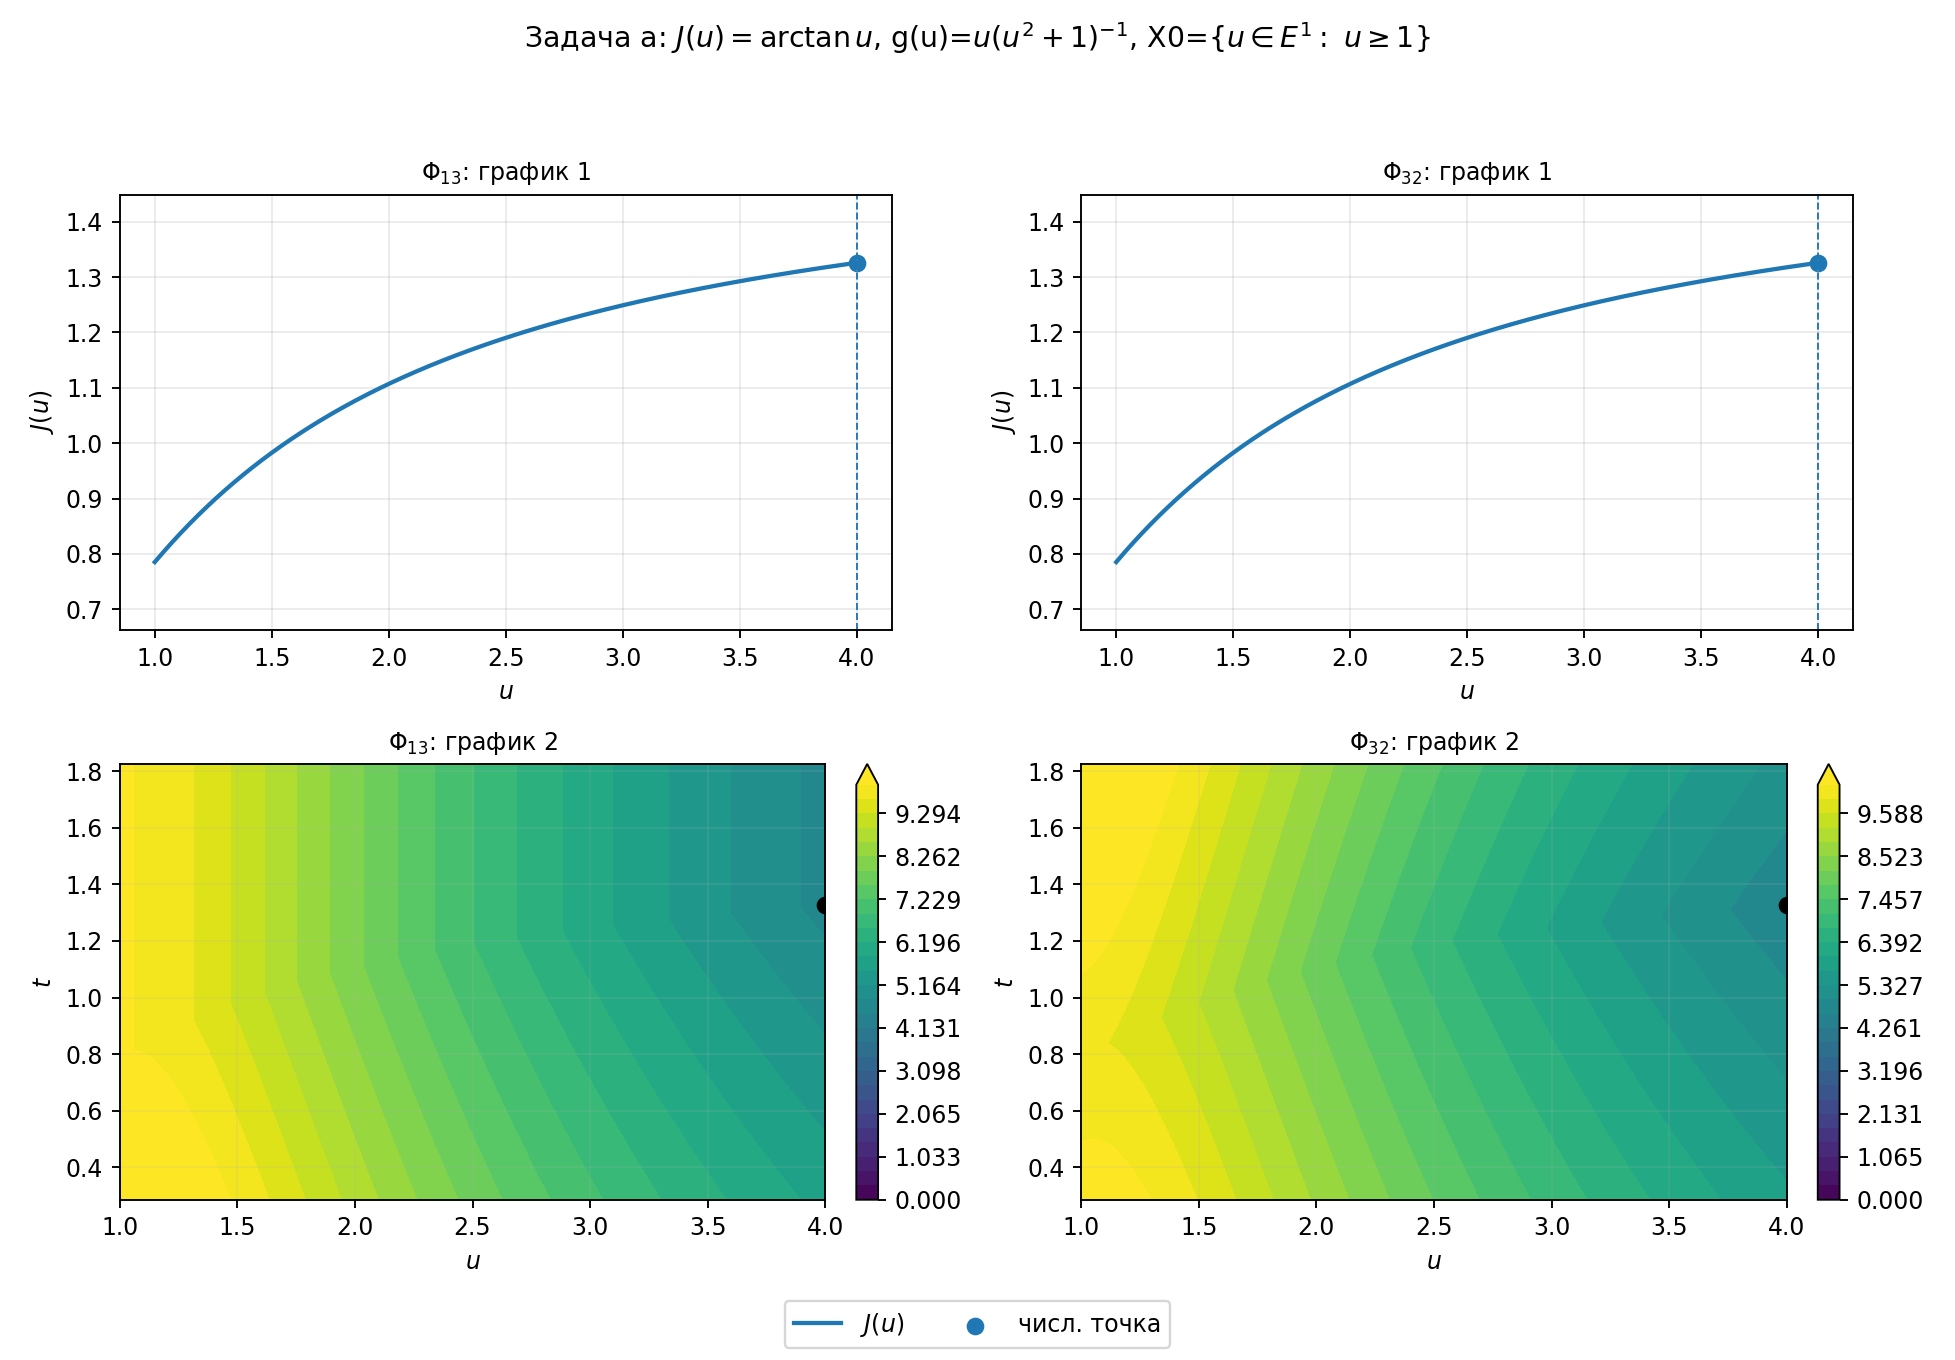
\includegraphics[width=0.96\textwidth]{graphs/a_g4_xge1_overview.png}
\caption{Задача а, вариант g4: $g(u)=u(u^2+1)^{-1}$, $X_0=\{u\in E^1:\ u\geq 1\}$. Верхний ряд: график 1 для $\Phi_{13}$ и $\Phi_{32}$; нижний ряд: график 2 для $\Phi_{13}$ и $\Phi_{32}$.}
\end{figure}

\begin{figure}[H]
\centering
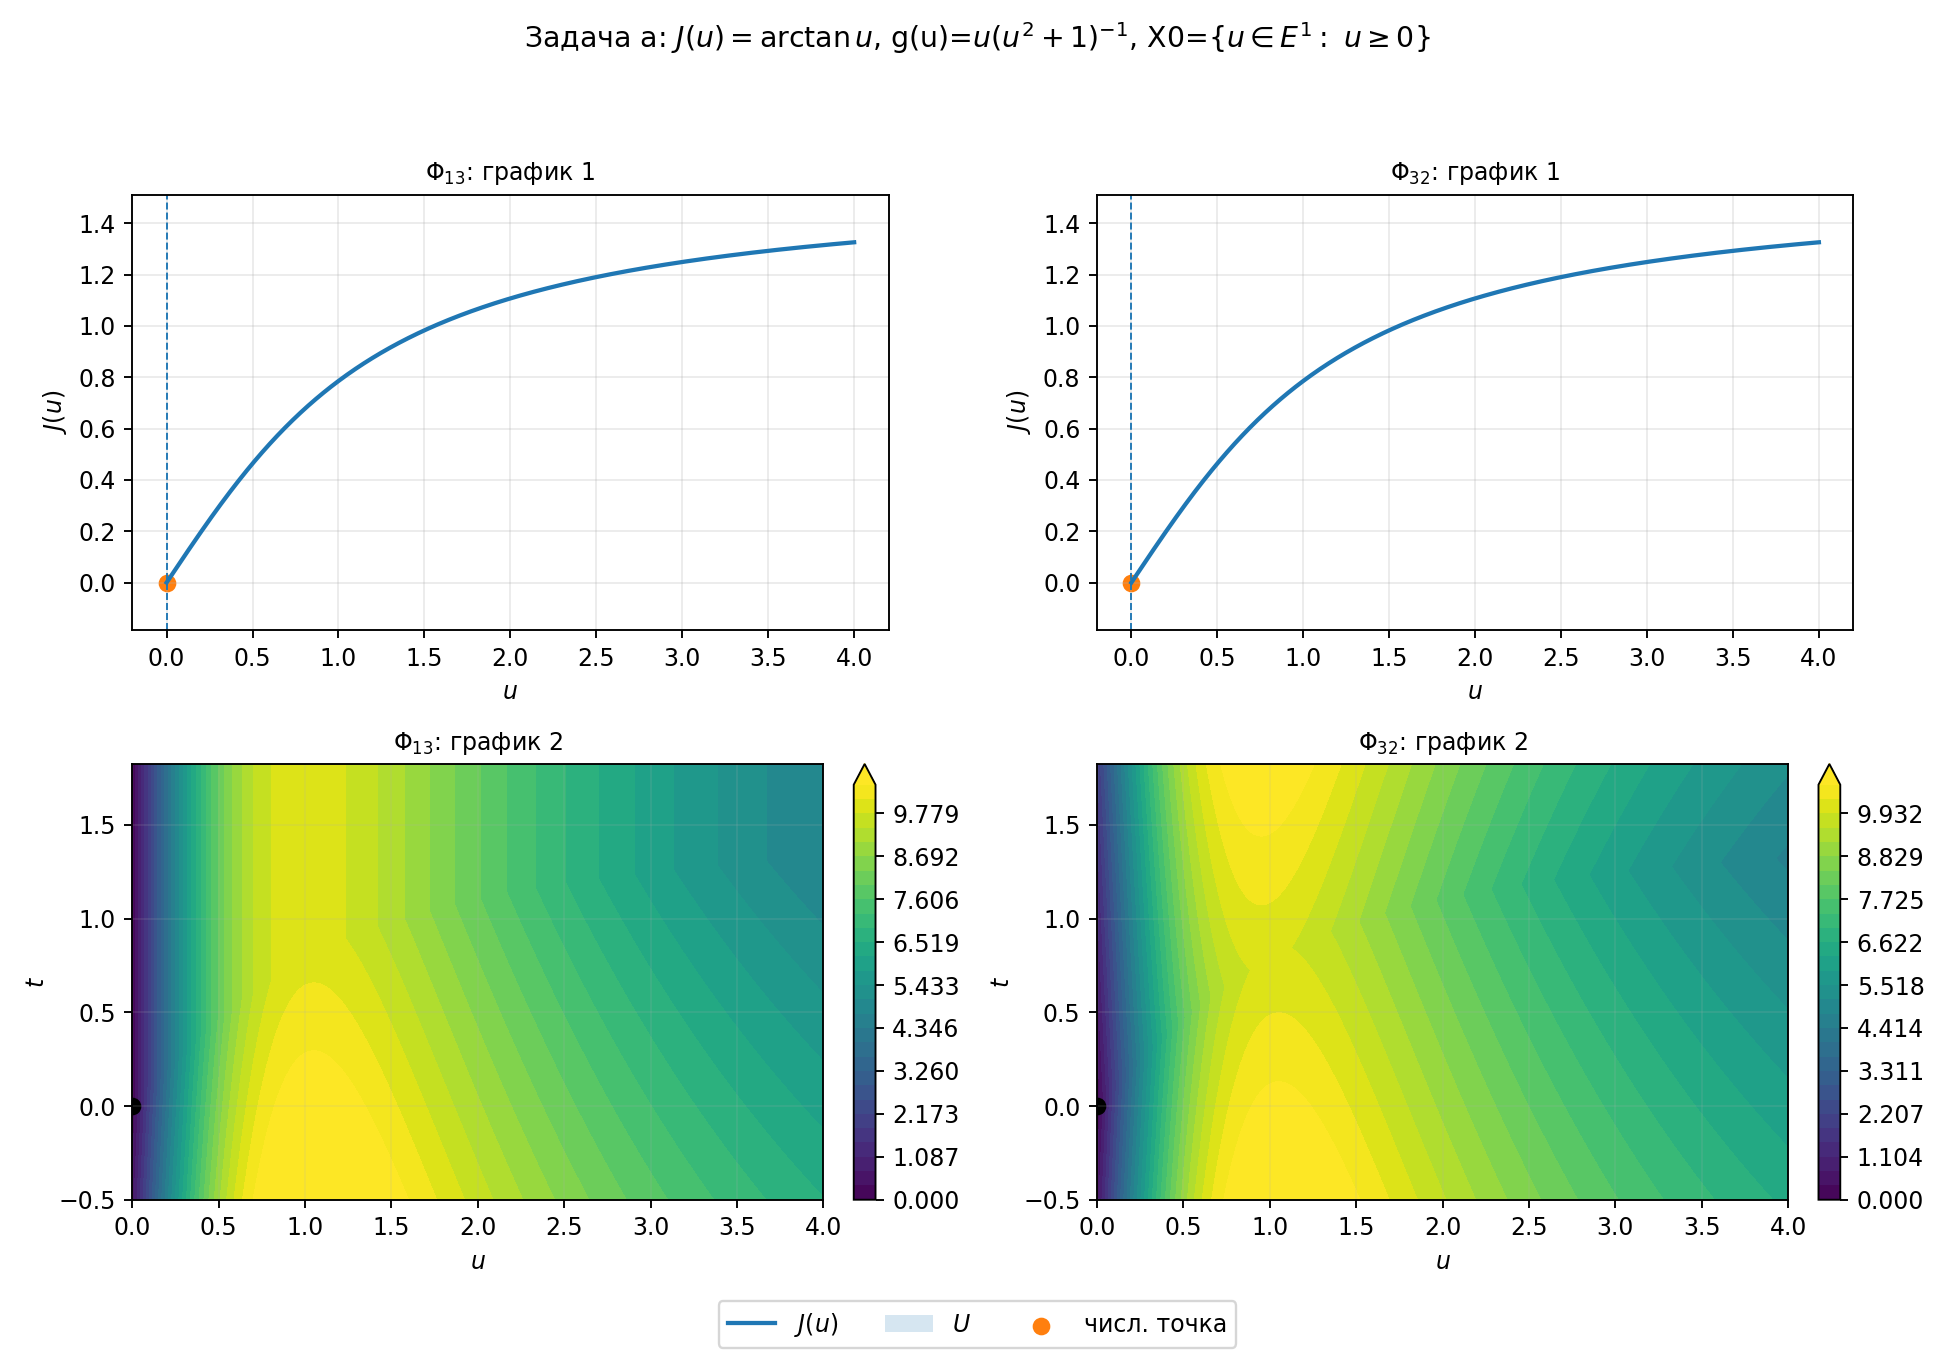
\includegraphics[width=0.96\textwidth]{graphs/a_g4_xge0_overview.png}
\caption{Задача а, вариант g4: $g(u)=u(u^2+1)^{-1}$, $X_0=\{u\in E^1:\ u\geq 0\}$. Верхний ряд: график 1 для $\Phi_{13}$ и $\Phi_{32}$; нижний ряд: график 2 для $\Phi_{13}$ и $\Phi_{32}$.}
\end{figure}

\begin{figure}[H]
\centering
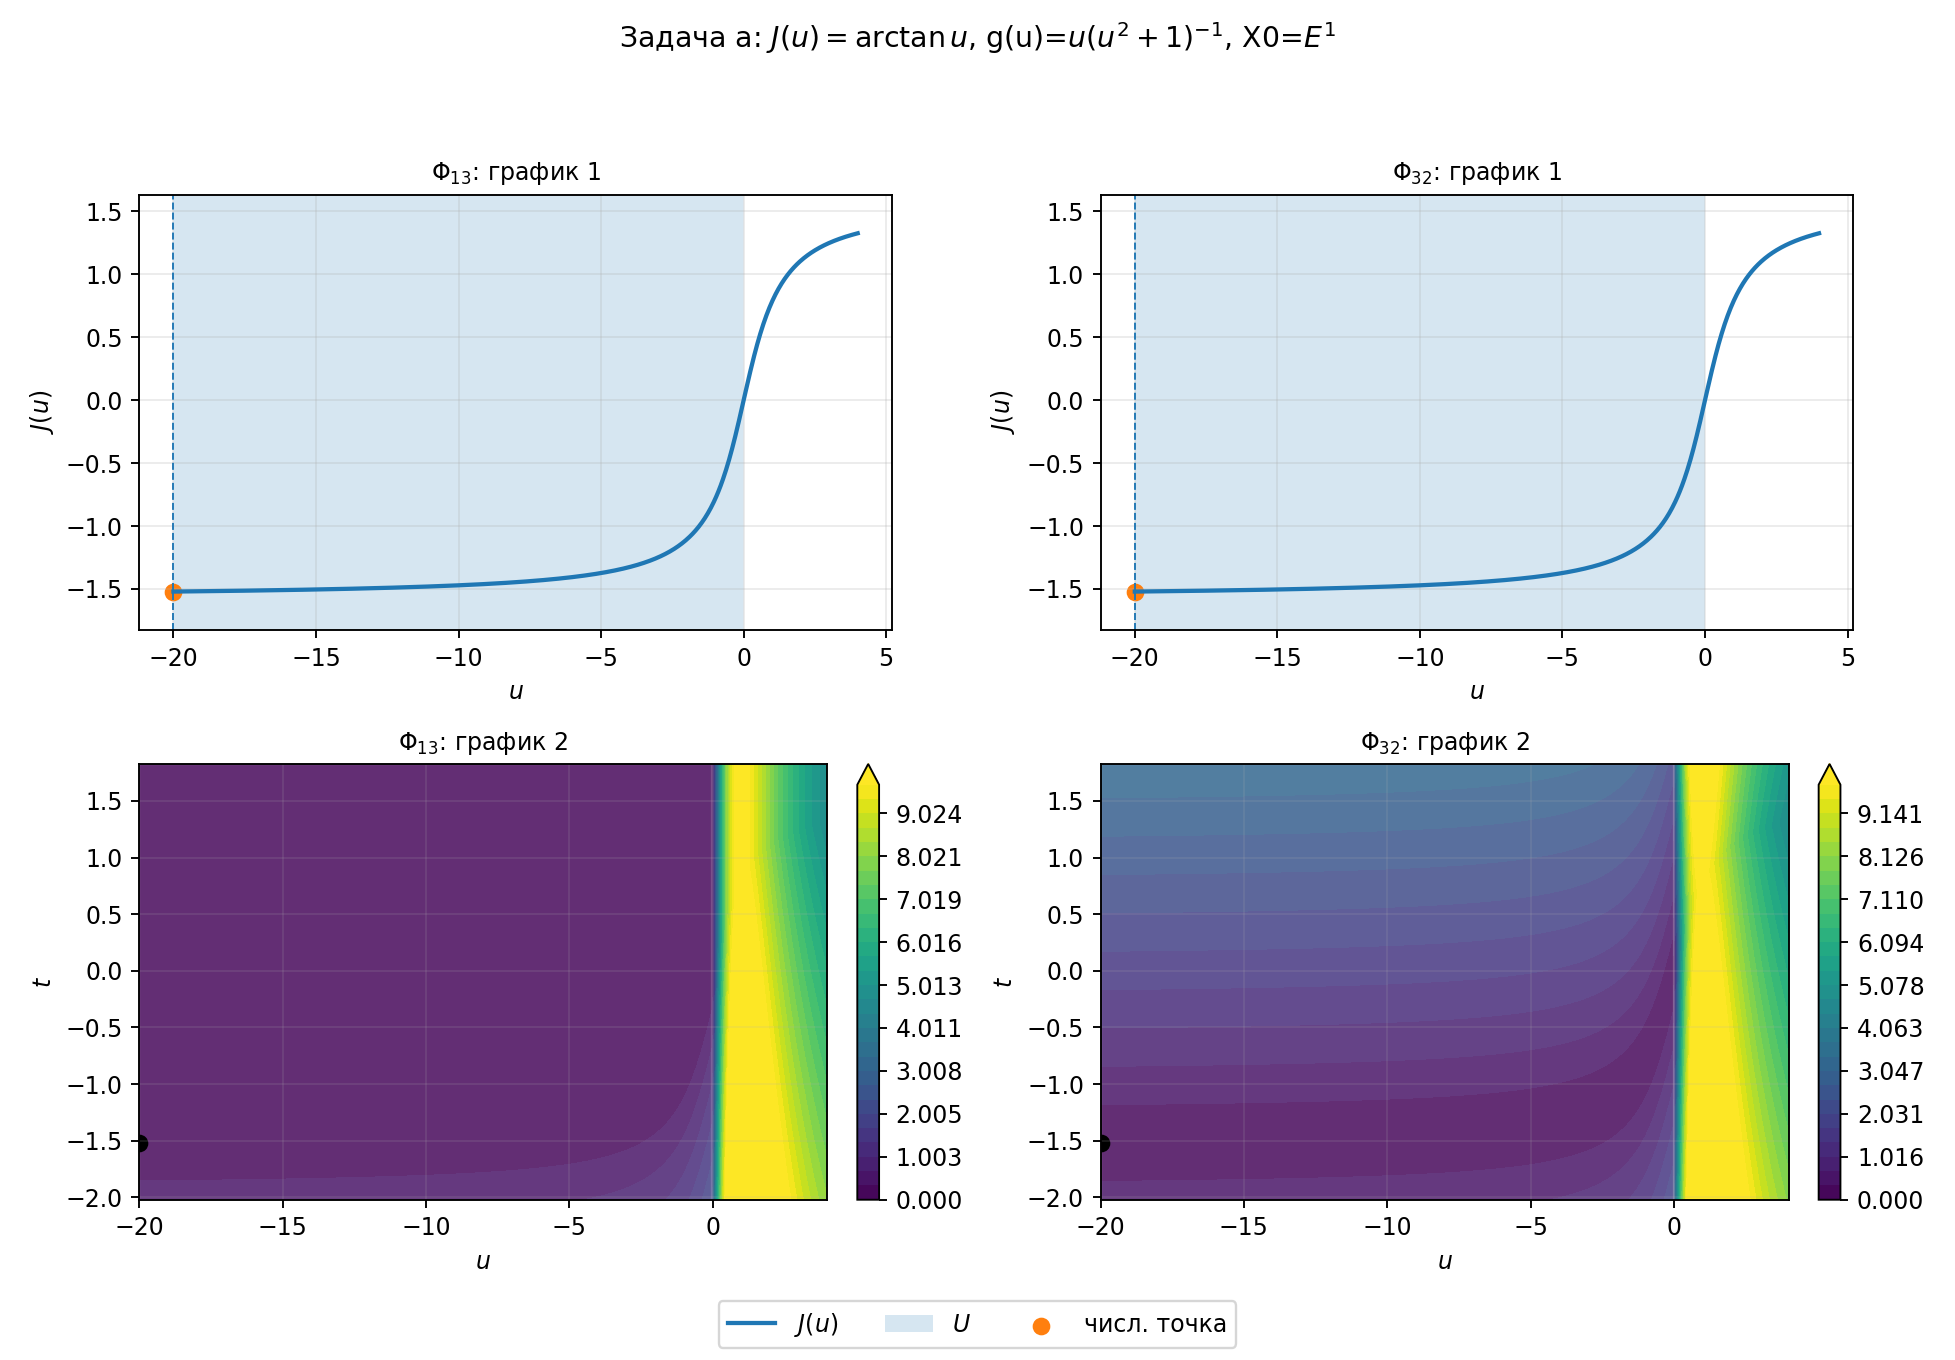
\includegraphics[width=0.96\textwidth]{graphs/a_g4_R_overview.png}
\caption{Задача а, вариант g4: $g(u)=u(u^2+1)^{-1}$, $X_0=E^1$. Верхний ряд: график 1 для $\Phi_{13}$ и $\Phi_{32}$; нижний ряд: график 2 для $\Phi_{13}$ и $\Phi_{32}$.}
\end{figure}

\begin{figure}[H]
\centering
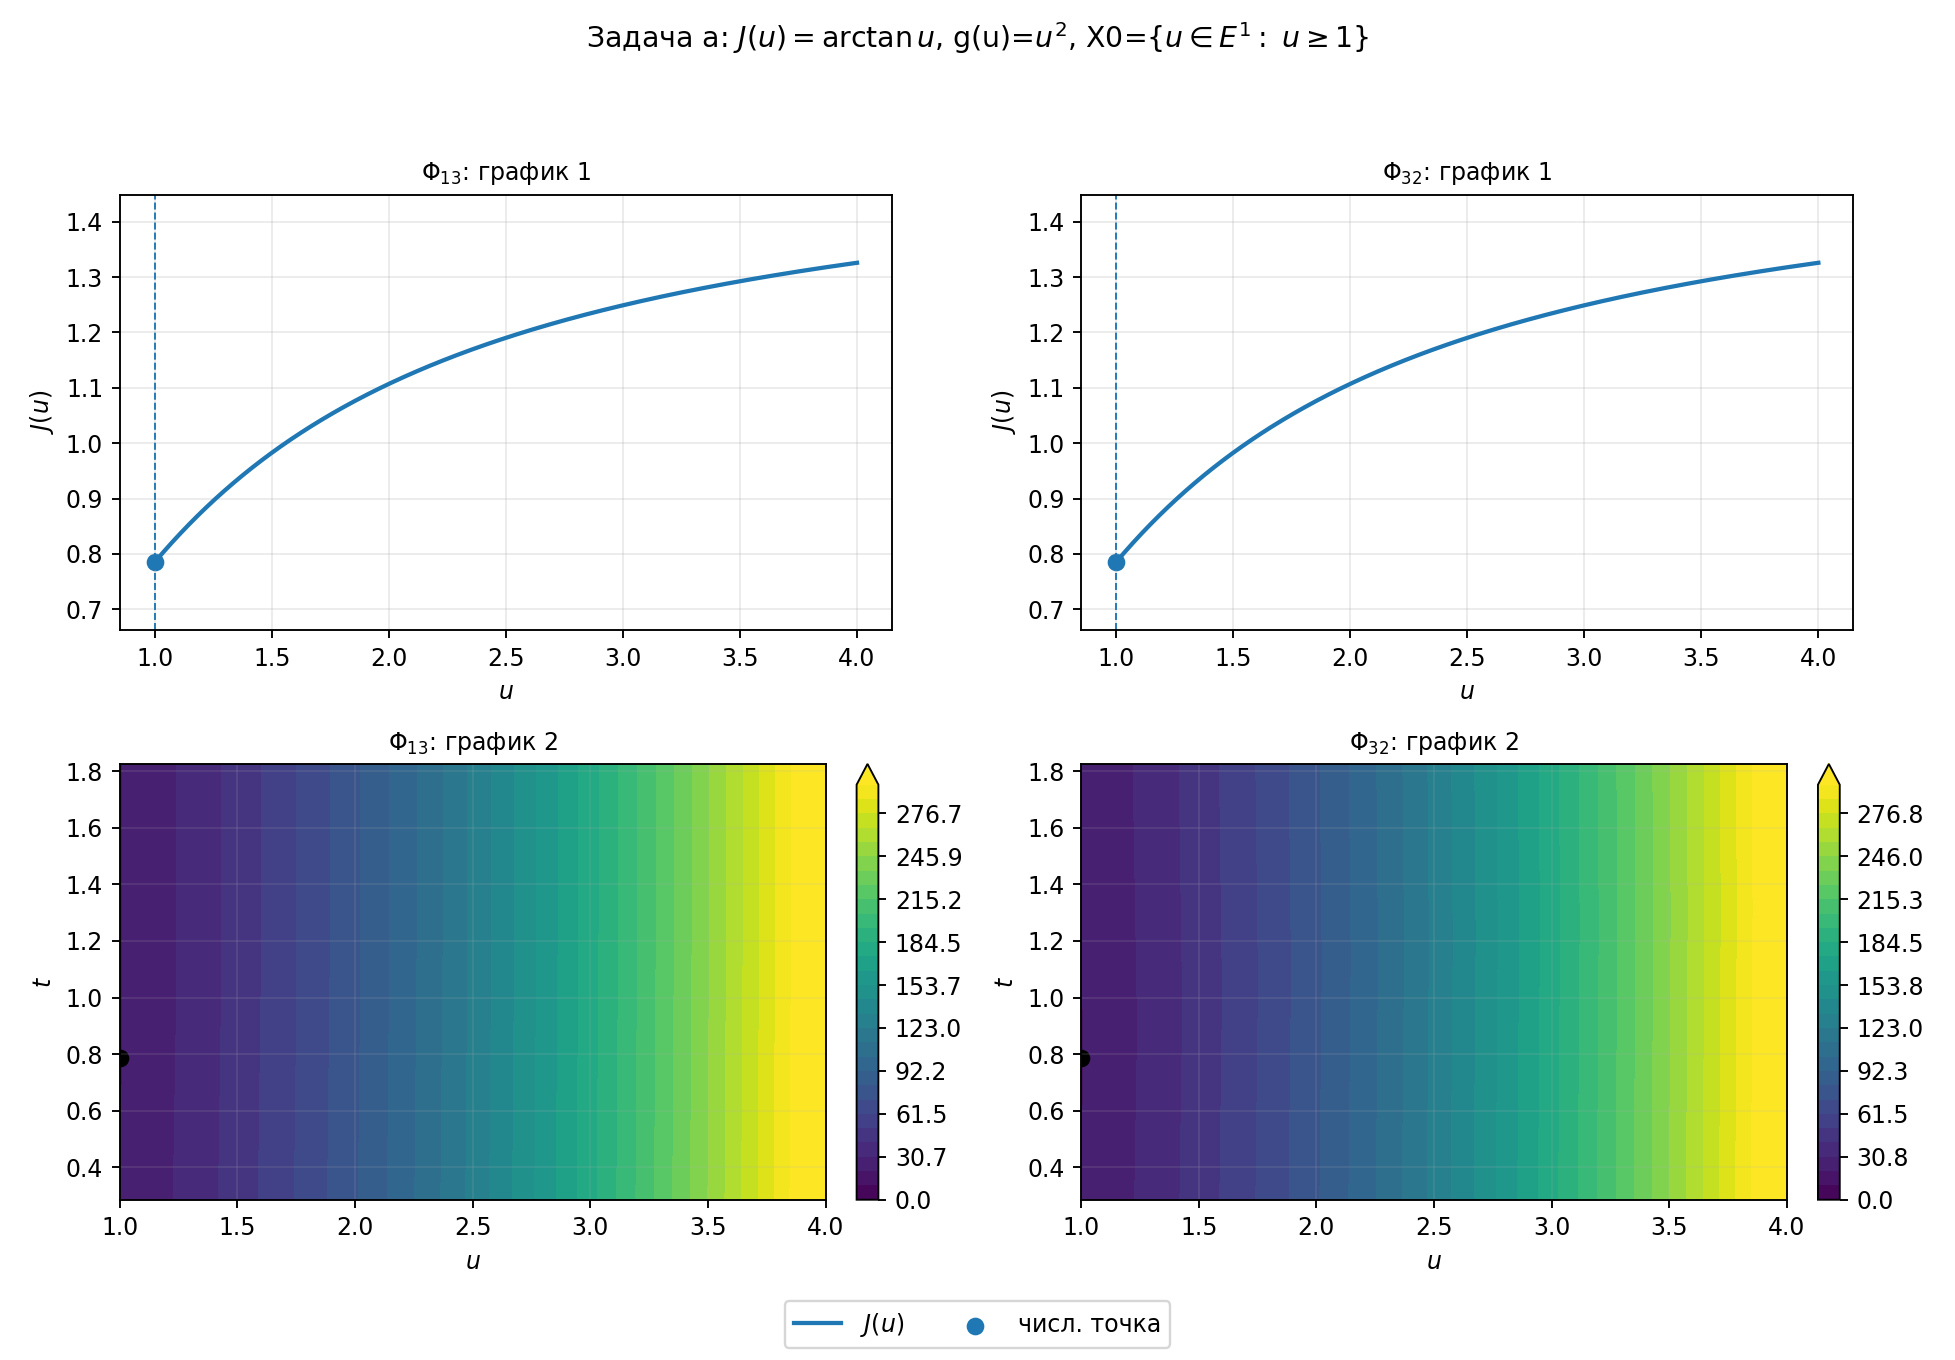
\includegraphics[width=0.96\textwidth]{graphs/a_g5_xge1_overview.png}
\caption{Задача а, вариант g5: $g(u)=u^2$, $X_0=\{u\in E^1:\ u\geq 1\}$. Верхний ряд: график 1 для $\Phi_{13}$ и $\Phi_{32}$; нижний ряд: график 2 для $\Phi_{13}$ и $\Phi_{32}$.}
\end{figure}

\begin{figure}[H]
\centering
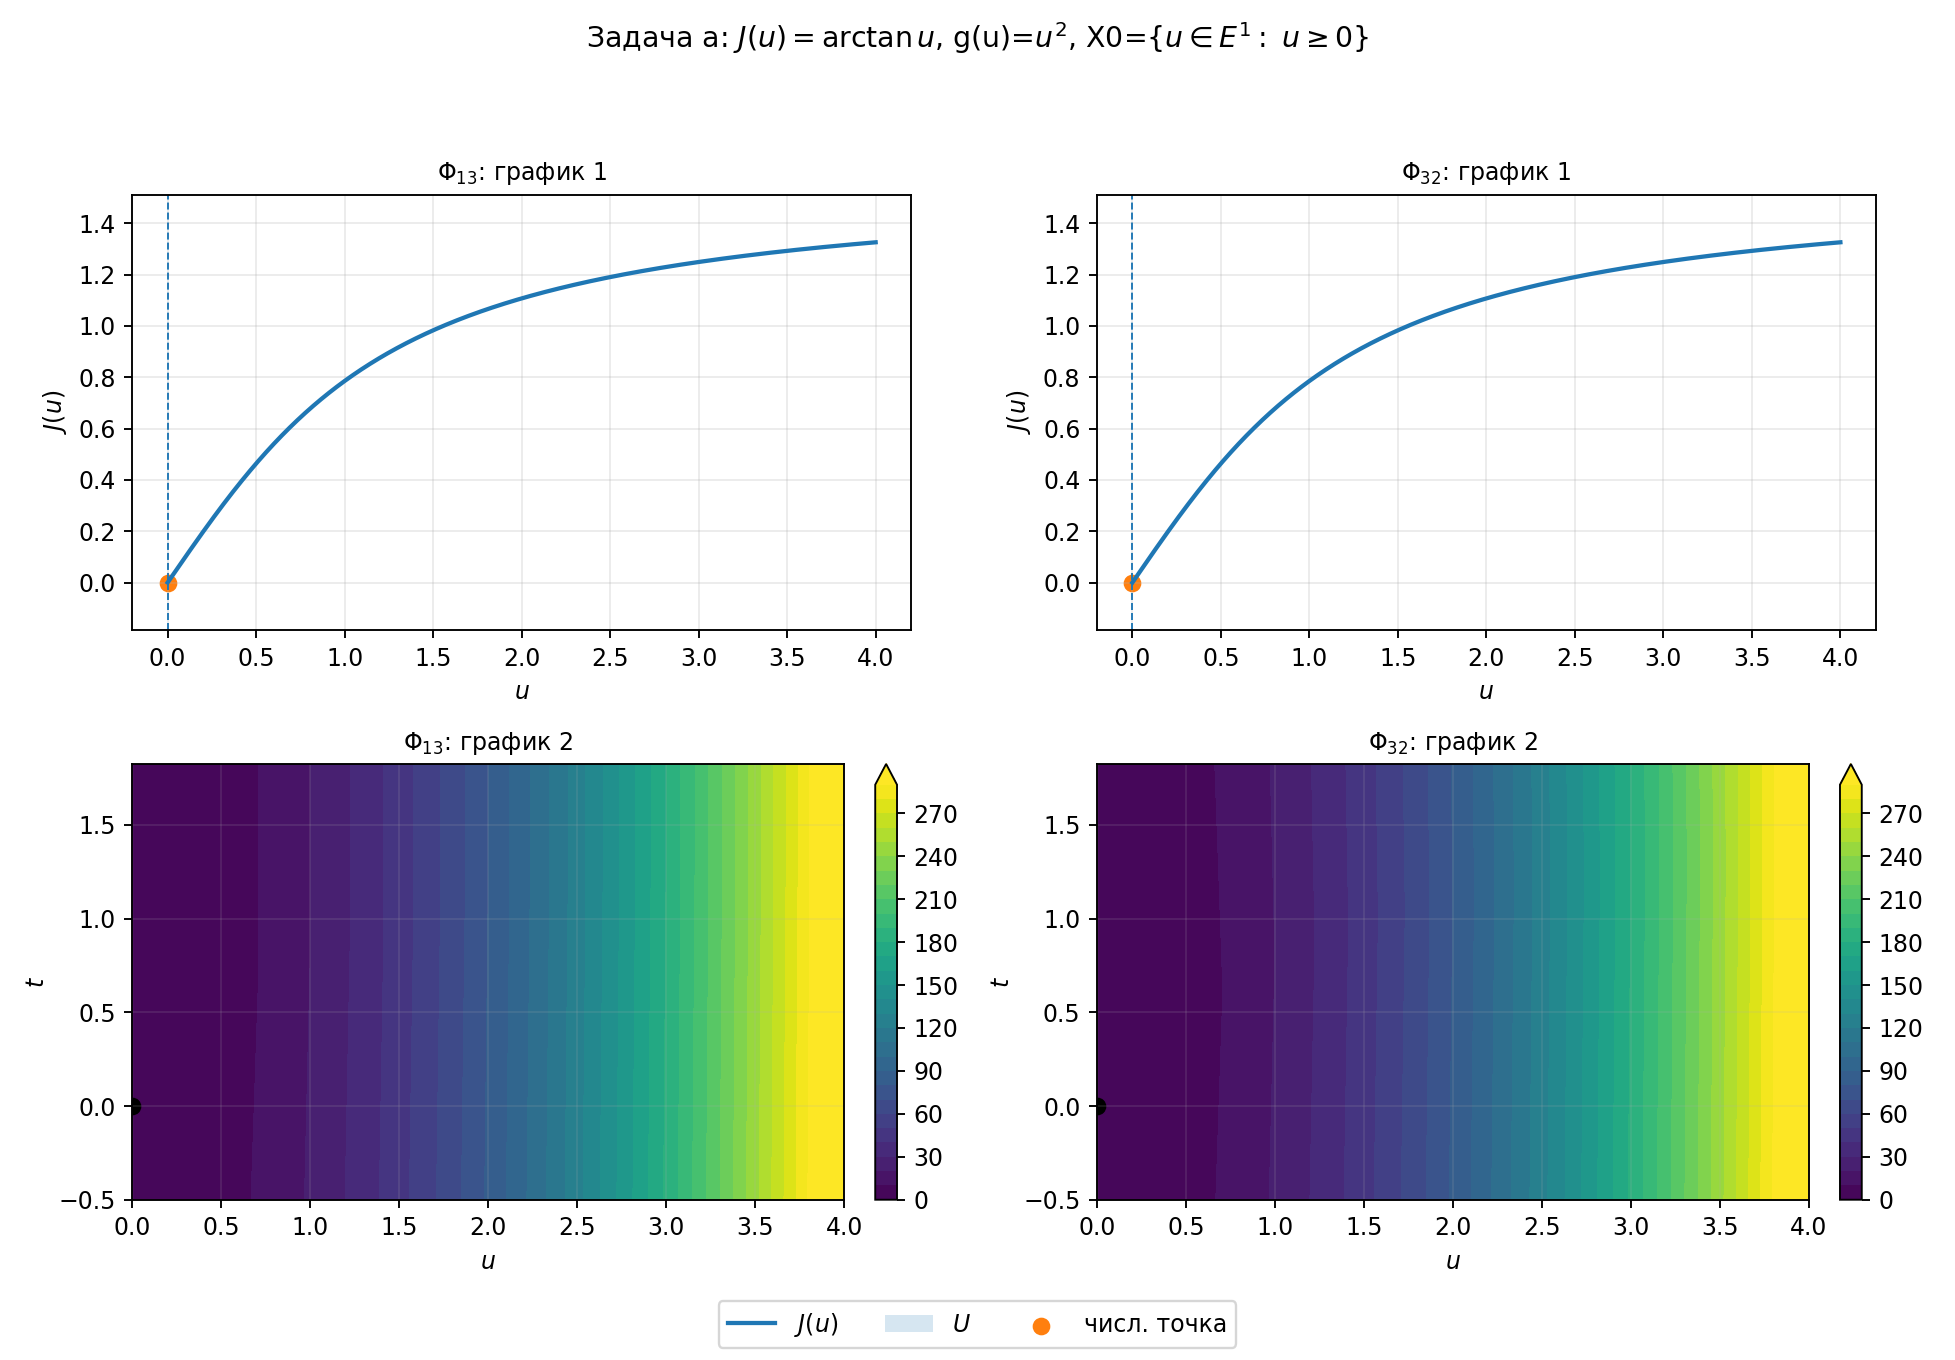
\includegraphics[width=0.96\textwidth]{graphs/a_g5_xge0_overview.png}
\caption{Задача а, вариант g5: $g(u)=u^2$, $X_0=\{u\in E^1:\ u\geq 0\}$. Верхний ряд: график 1 для $\Phi_{13}$ и $\Phi_{32}$; нижний ряд: график 2 для $\Phi_{13}$ и $\Phi_{32}$.}
\end{figure}

\begin{figure}[H]
\centering
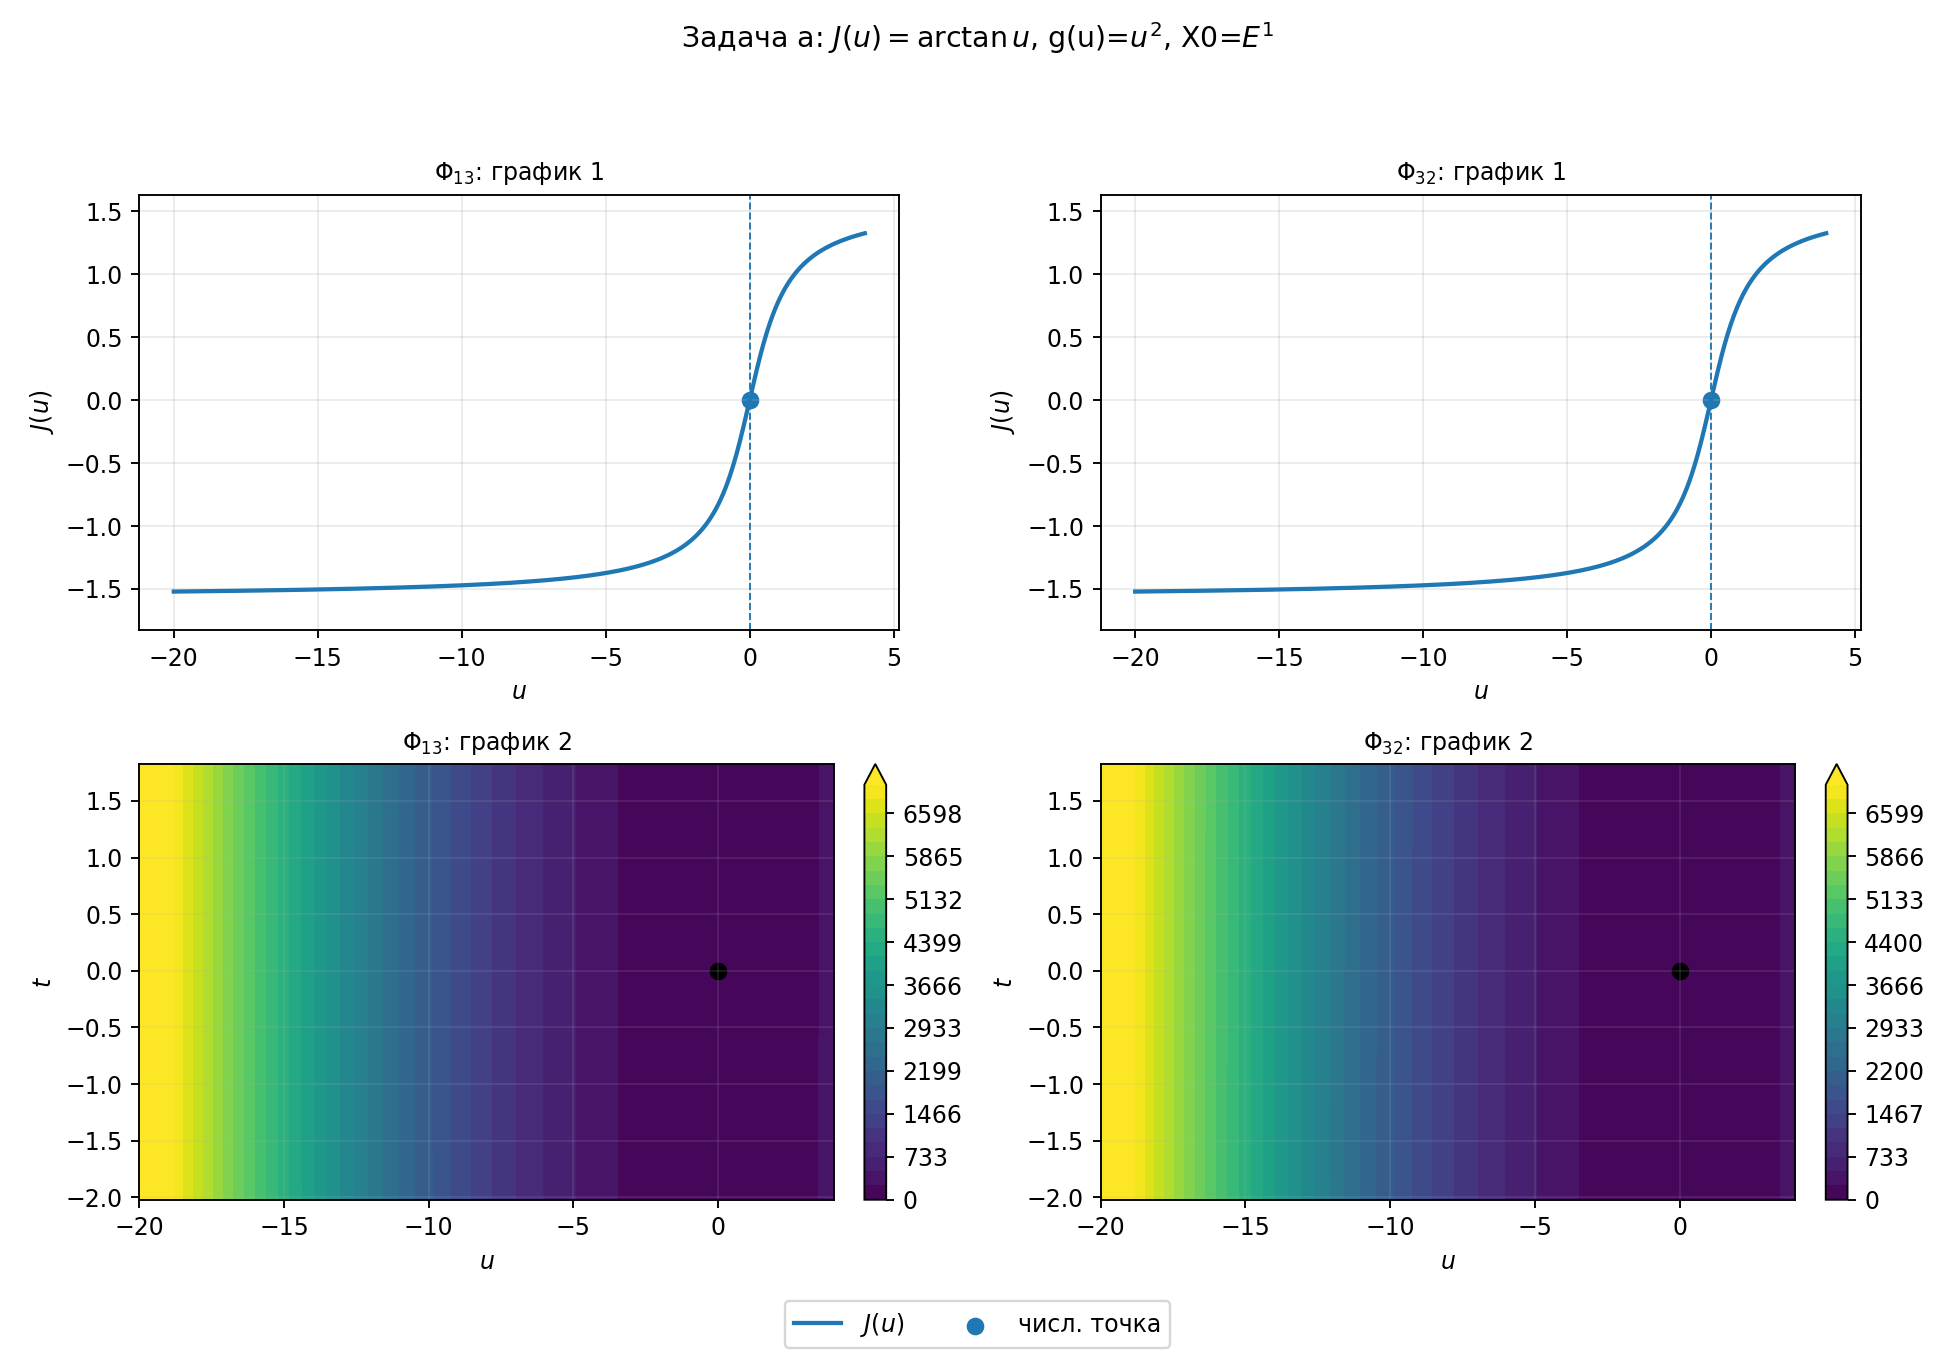
\includegraphics[width=0.96\textwidth]{graphs/a_g5_R_overview.png}
\caption{Задача а, вариант g5: $g(u)=u^2$, $X_0=E^1$. Верхний ряд: график 1 для $\Phi_{13}$ и $\Phi_{32}$; нижний ряд: график 2 для $\Phi_{13}$ и $\Phi_{32}$.}
\end{figure}

\begin{figure}[H]
\centering
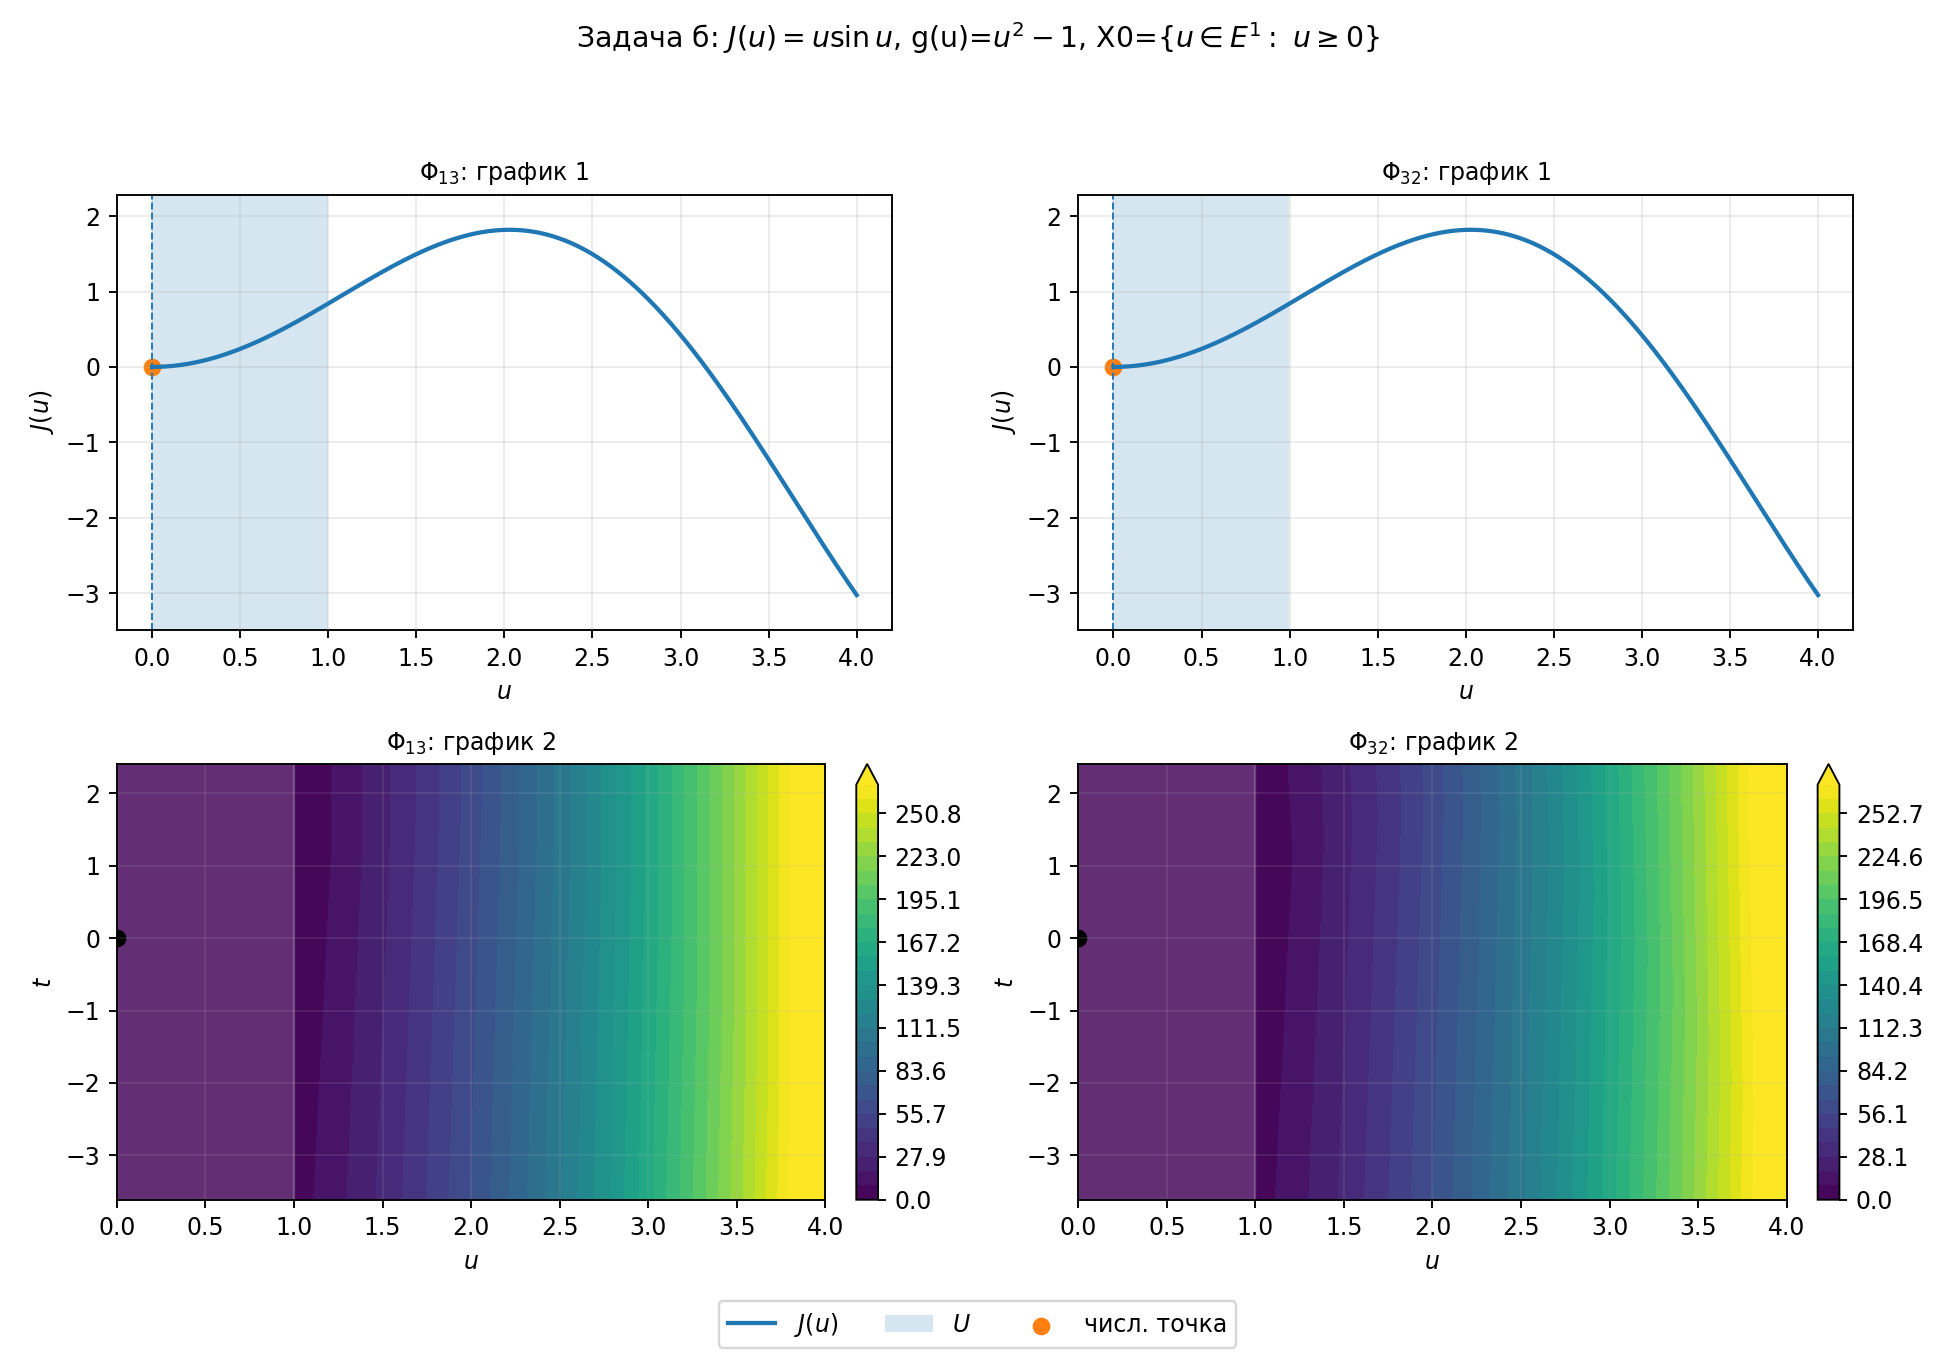
\includegraphics[width=0.96\textwidth]{graphs/b_g1_xge0_overview.png}
\caption{Задача б, вариант g1: $g(u)=u^2-1$, $X_0=\{u\in E^1:\ u\geq 0\}$. Верхний ряд: график 1 для $\Phi_{13}$ и $\Phi_{32}$; нижний ряд: график 2 для $\Phi_{13}$ и $\Phi_{32}$.}
\end{figure}

\begin{figure}[H]
\centering
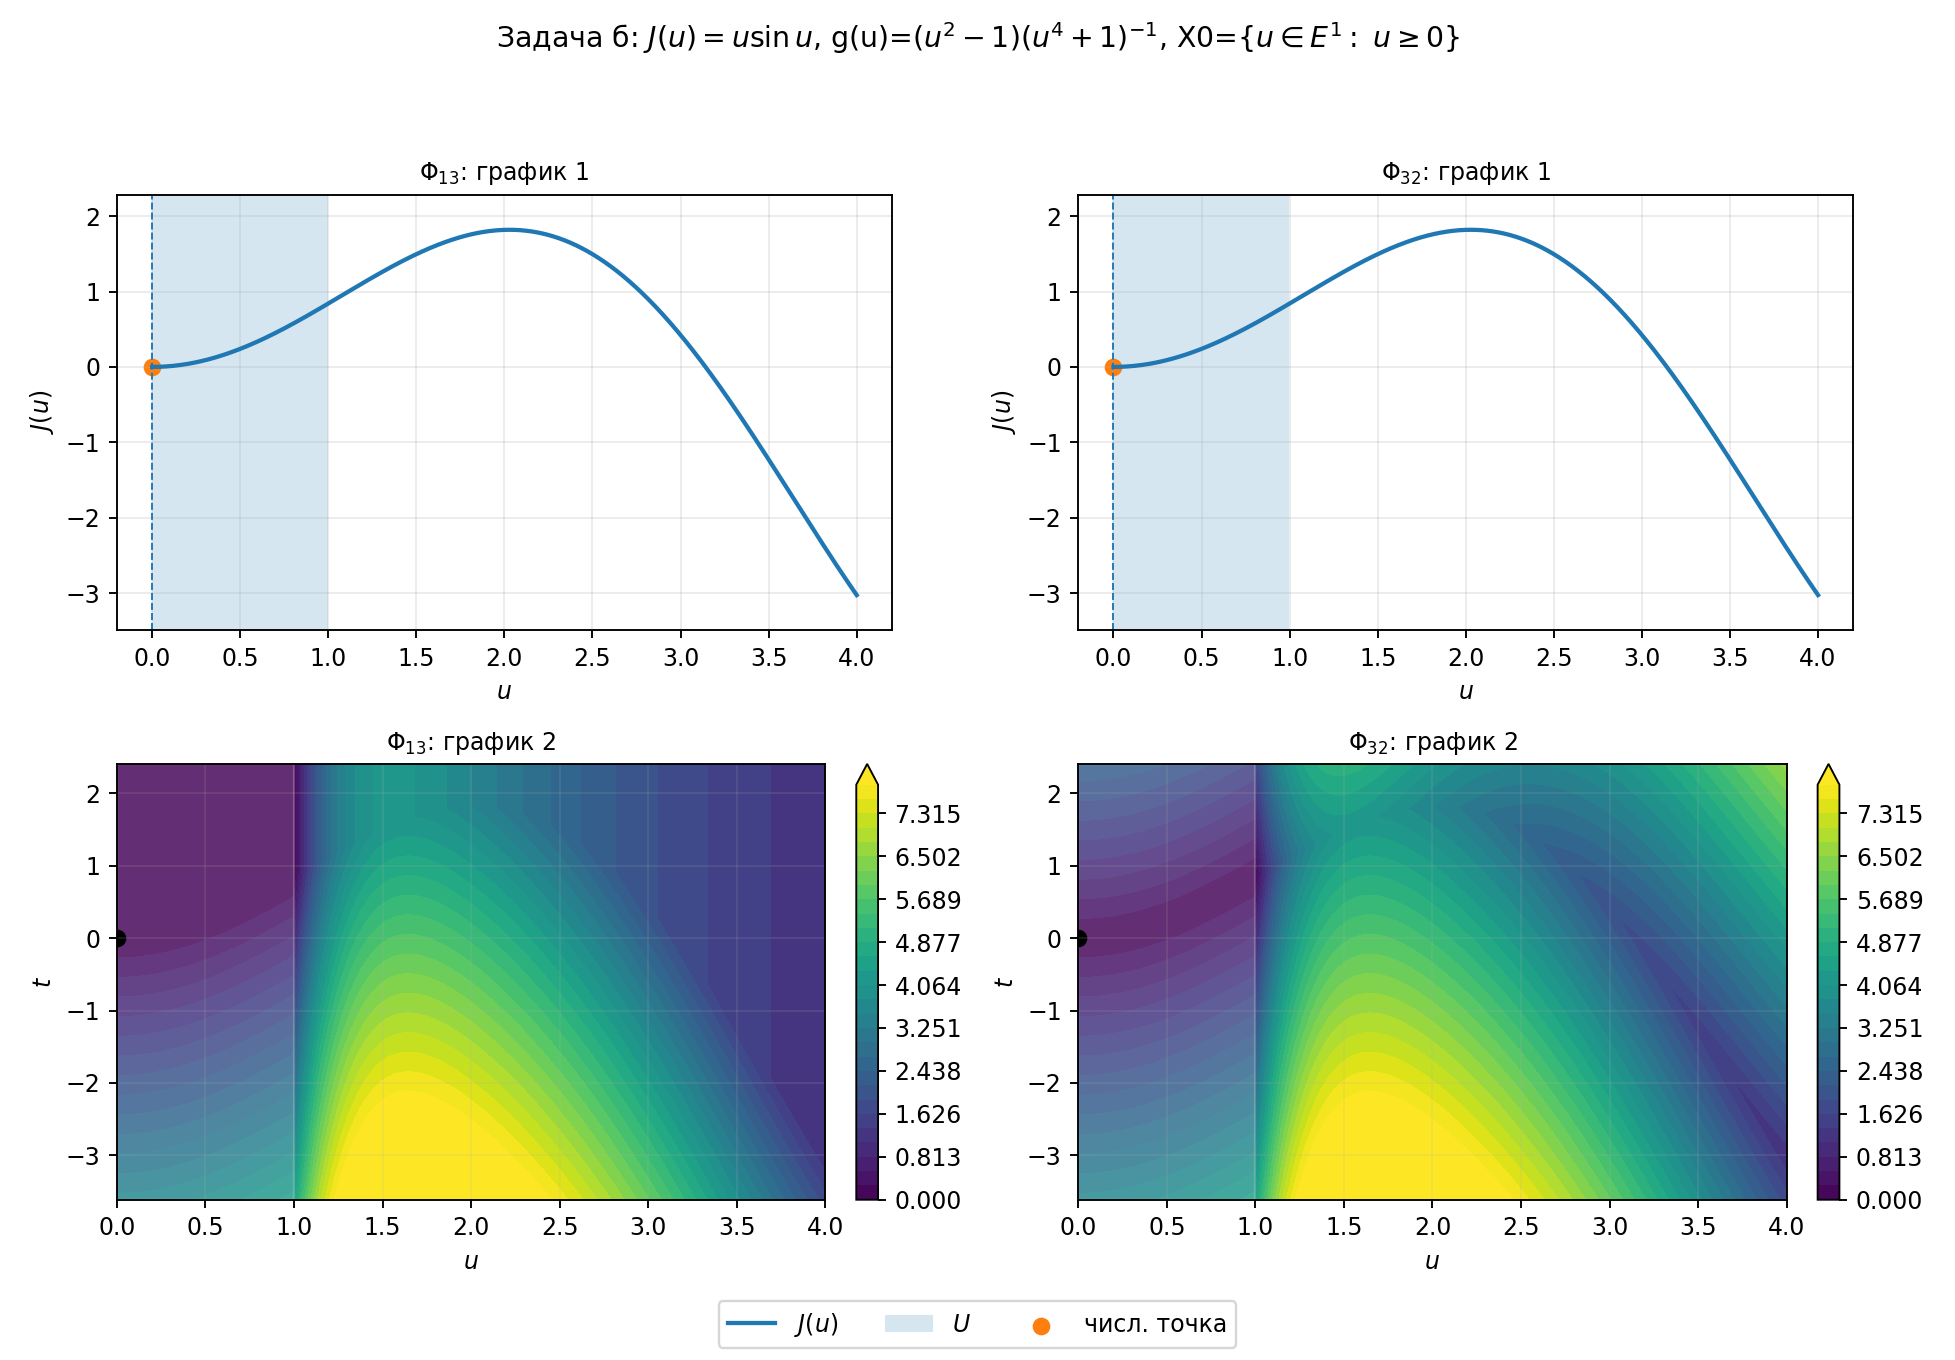
\includegraphics[width=0.96\textwidth]{graphs/b_g2_xge0_overview.png}
\caption{Задача б, вариант g2: $g(u)=(u^2-1)(u^4+1)^{-1}$, $X_0=\{u\in E^1:\ u\geq 0\}$. Верхний ряд: график 1 для $\Phi_{13}$ и $\Phi_{32}$; нижний ряд: график 2 для $\Phi_{13}$ и $\Phi_{32}$.}
\end{figure}

\begin{figure}[H]
\centering
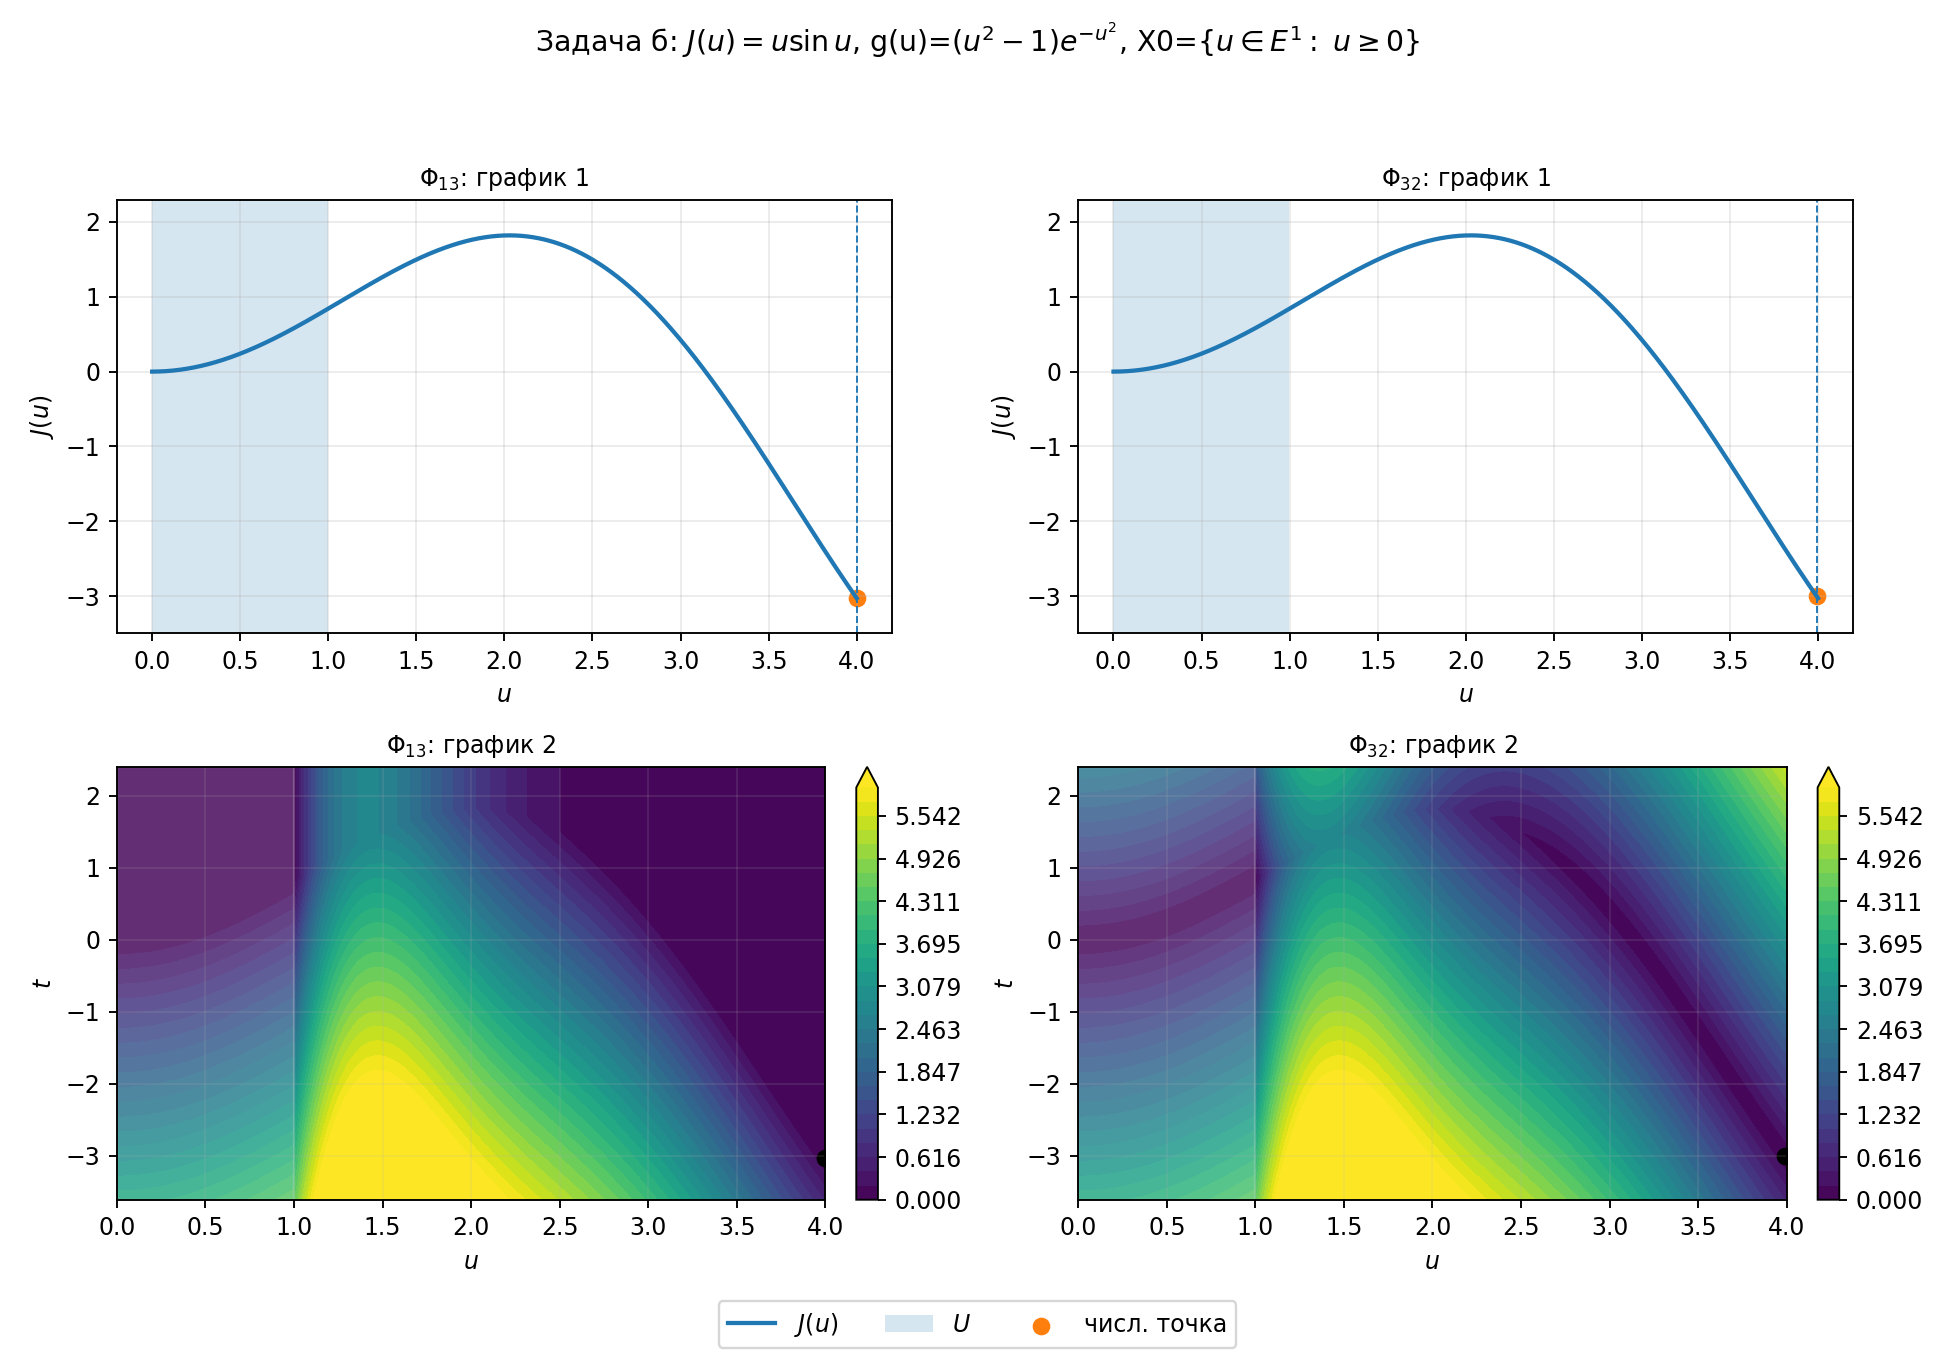
\includegraphics[width=0.96\textwidth]{graphs/b_g3_xge0_overview.png}
\caption{Задача б, вариант g3: $g(u)=(u^2-1)e^{-u^2}$, $X_0=\{u\in E^1:\ u\geq 0\}$. Верхний ряд: график 1 для $\Phi_{13}$ и $\Phi_{32}$; нижний ряд: график 2 для $\Phi_{13}$ и $\Phi_{32}$.}
\end{figure}

\begin{figure}[H]
\centering
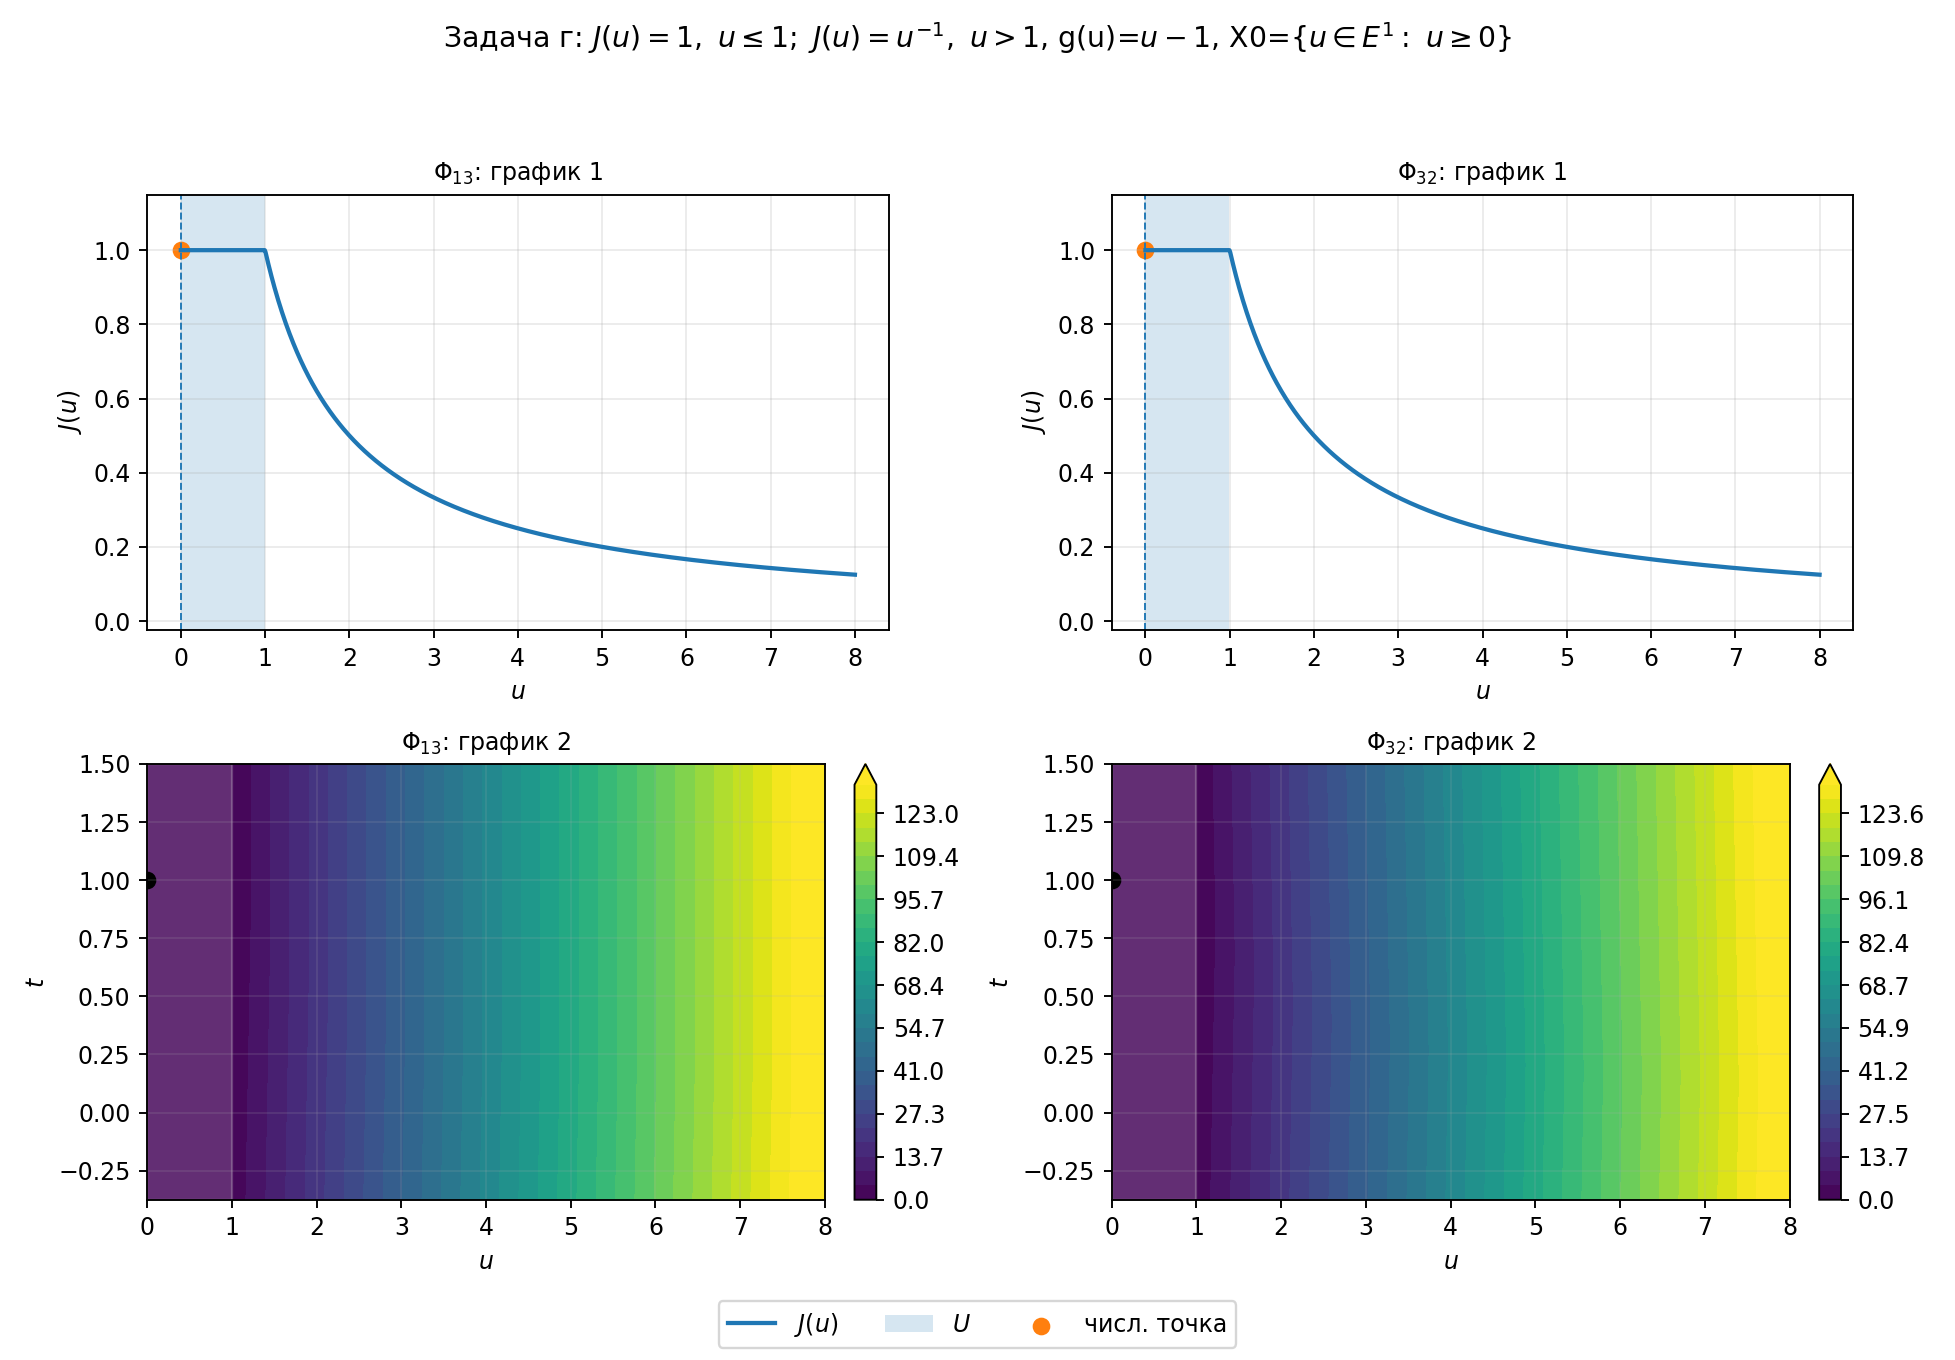
\includegraphics[width=0.96\textwidth]{graphs/g_g1_xge0_overview.png}
\caption{Задача г, вариант g1: $g(u)=u-1$, $X_0=\{u\in E^1:\ u\geq 0\}$. Верхний ряд: график 1 для $\Phi_{13}$ и $\Phi_{32}$; нижний ряд: график 2 для $\Phi_{13}$ и $\Phi_{32}$.}
\end{figure}

\begin{figure}[H]
\centering
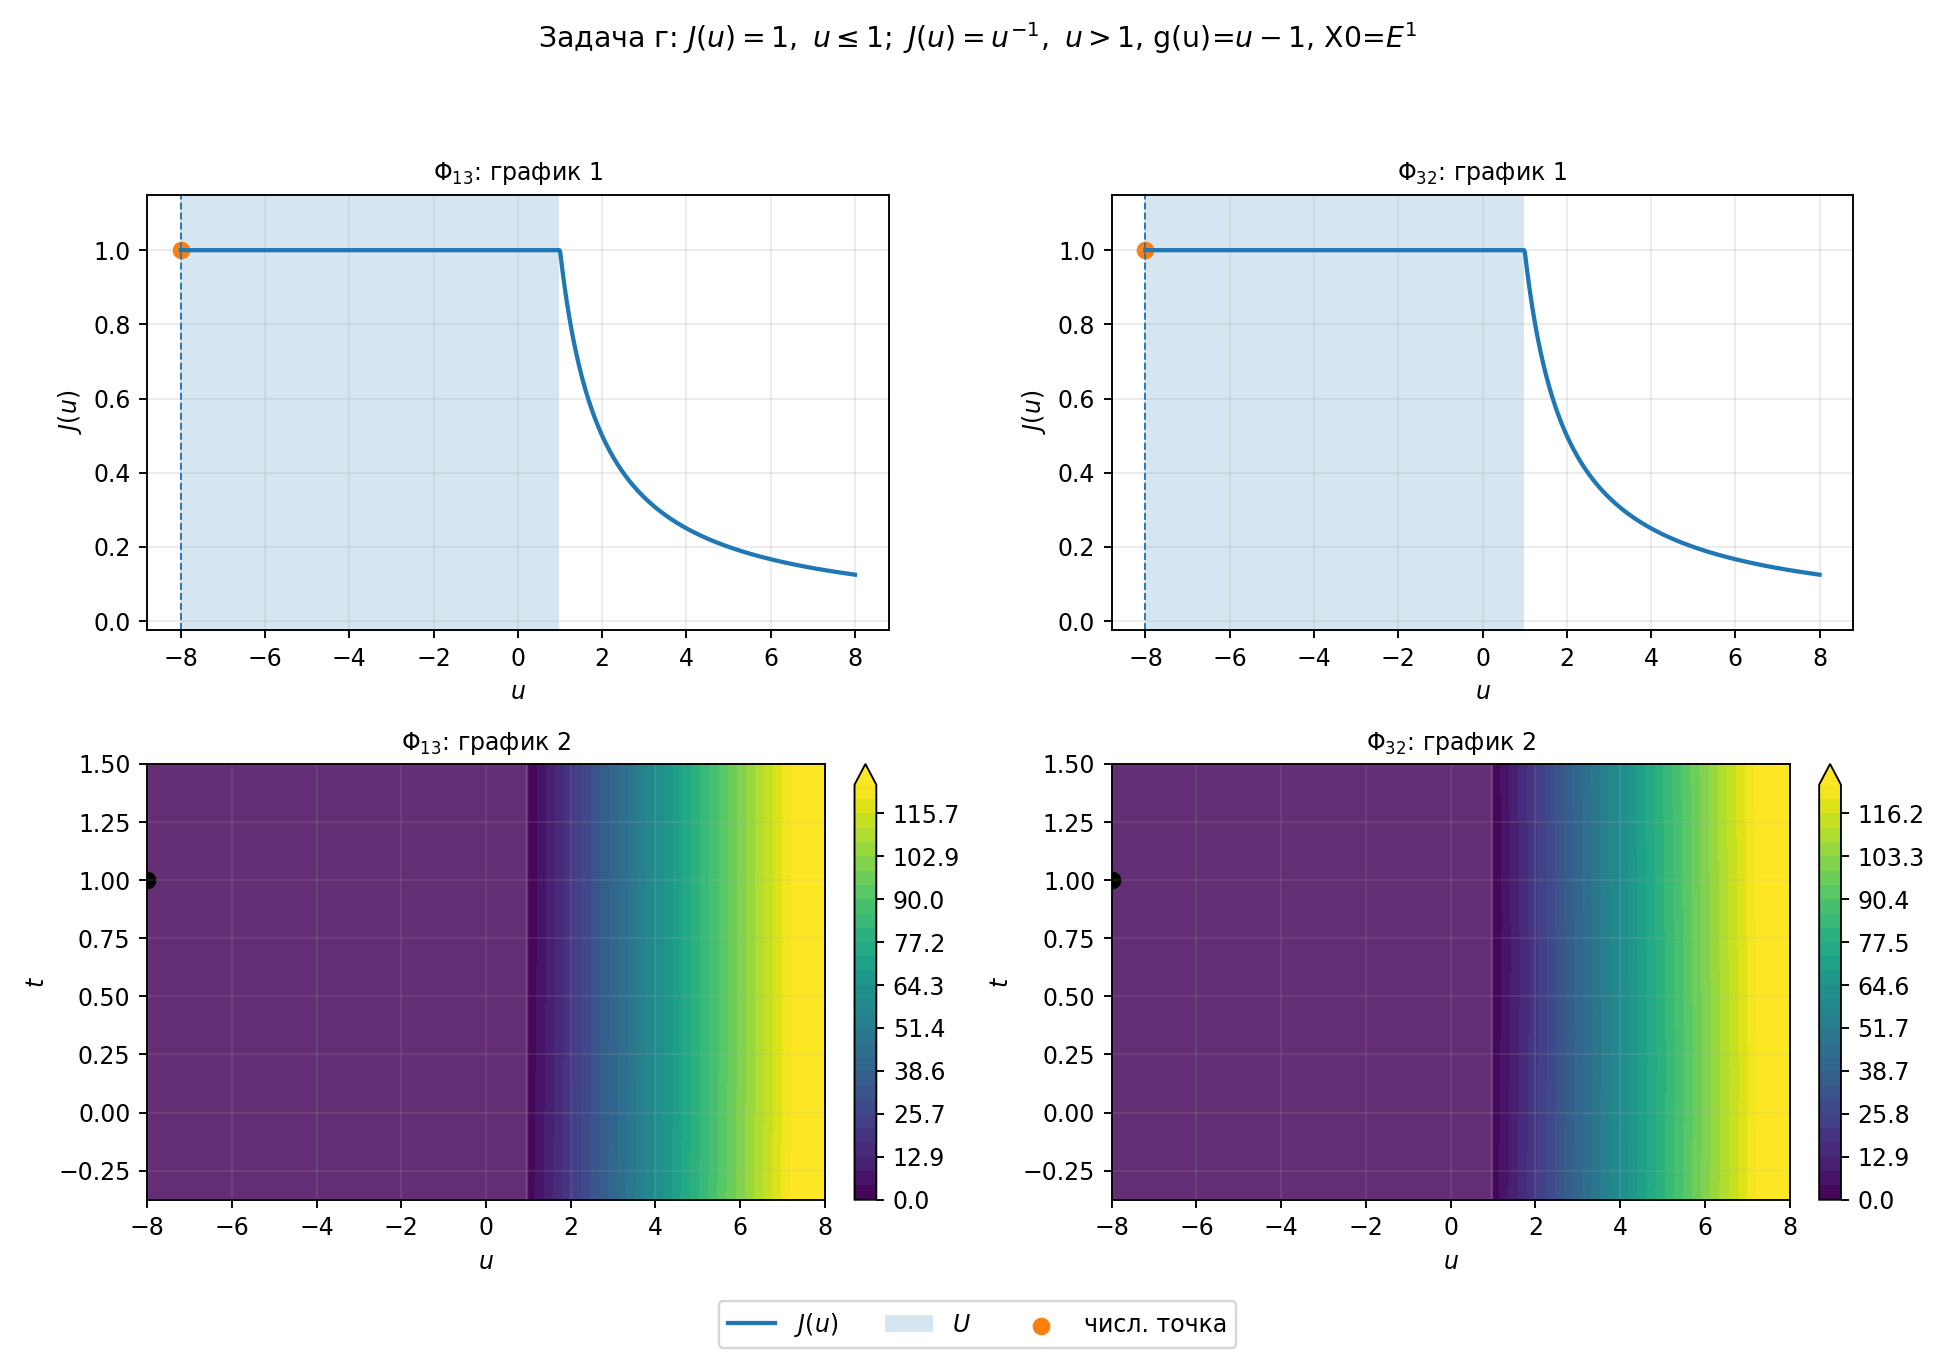
\includegraphics[width=0.96\textwidth]{graphs/g_g1_R_overview.png}
\caption{Задача г, вариант g1: $g(u)=u-1$, $X_0=E^1$. Верхний ряд: график 1 для $\Phi_{13}$ и $\Phi_{32}$; нижний ряд: график 2 для $\Phi_{13}$ и $\Phi_{32}$.}
\end{figure}

\begin{figure}[H]
\centering
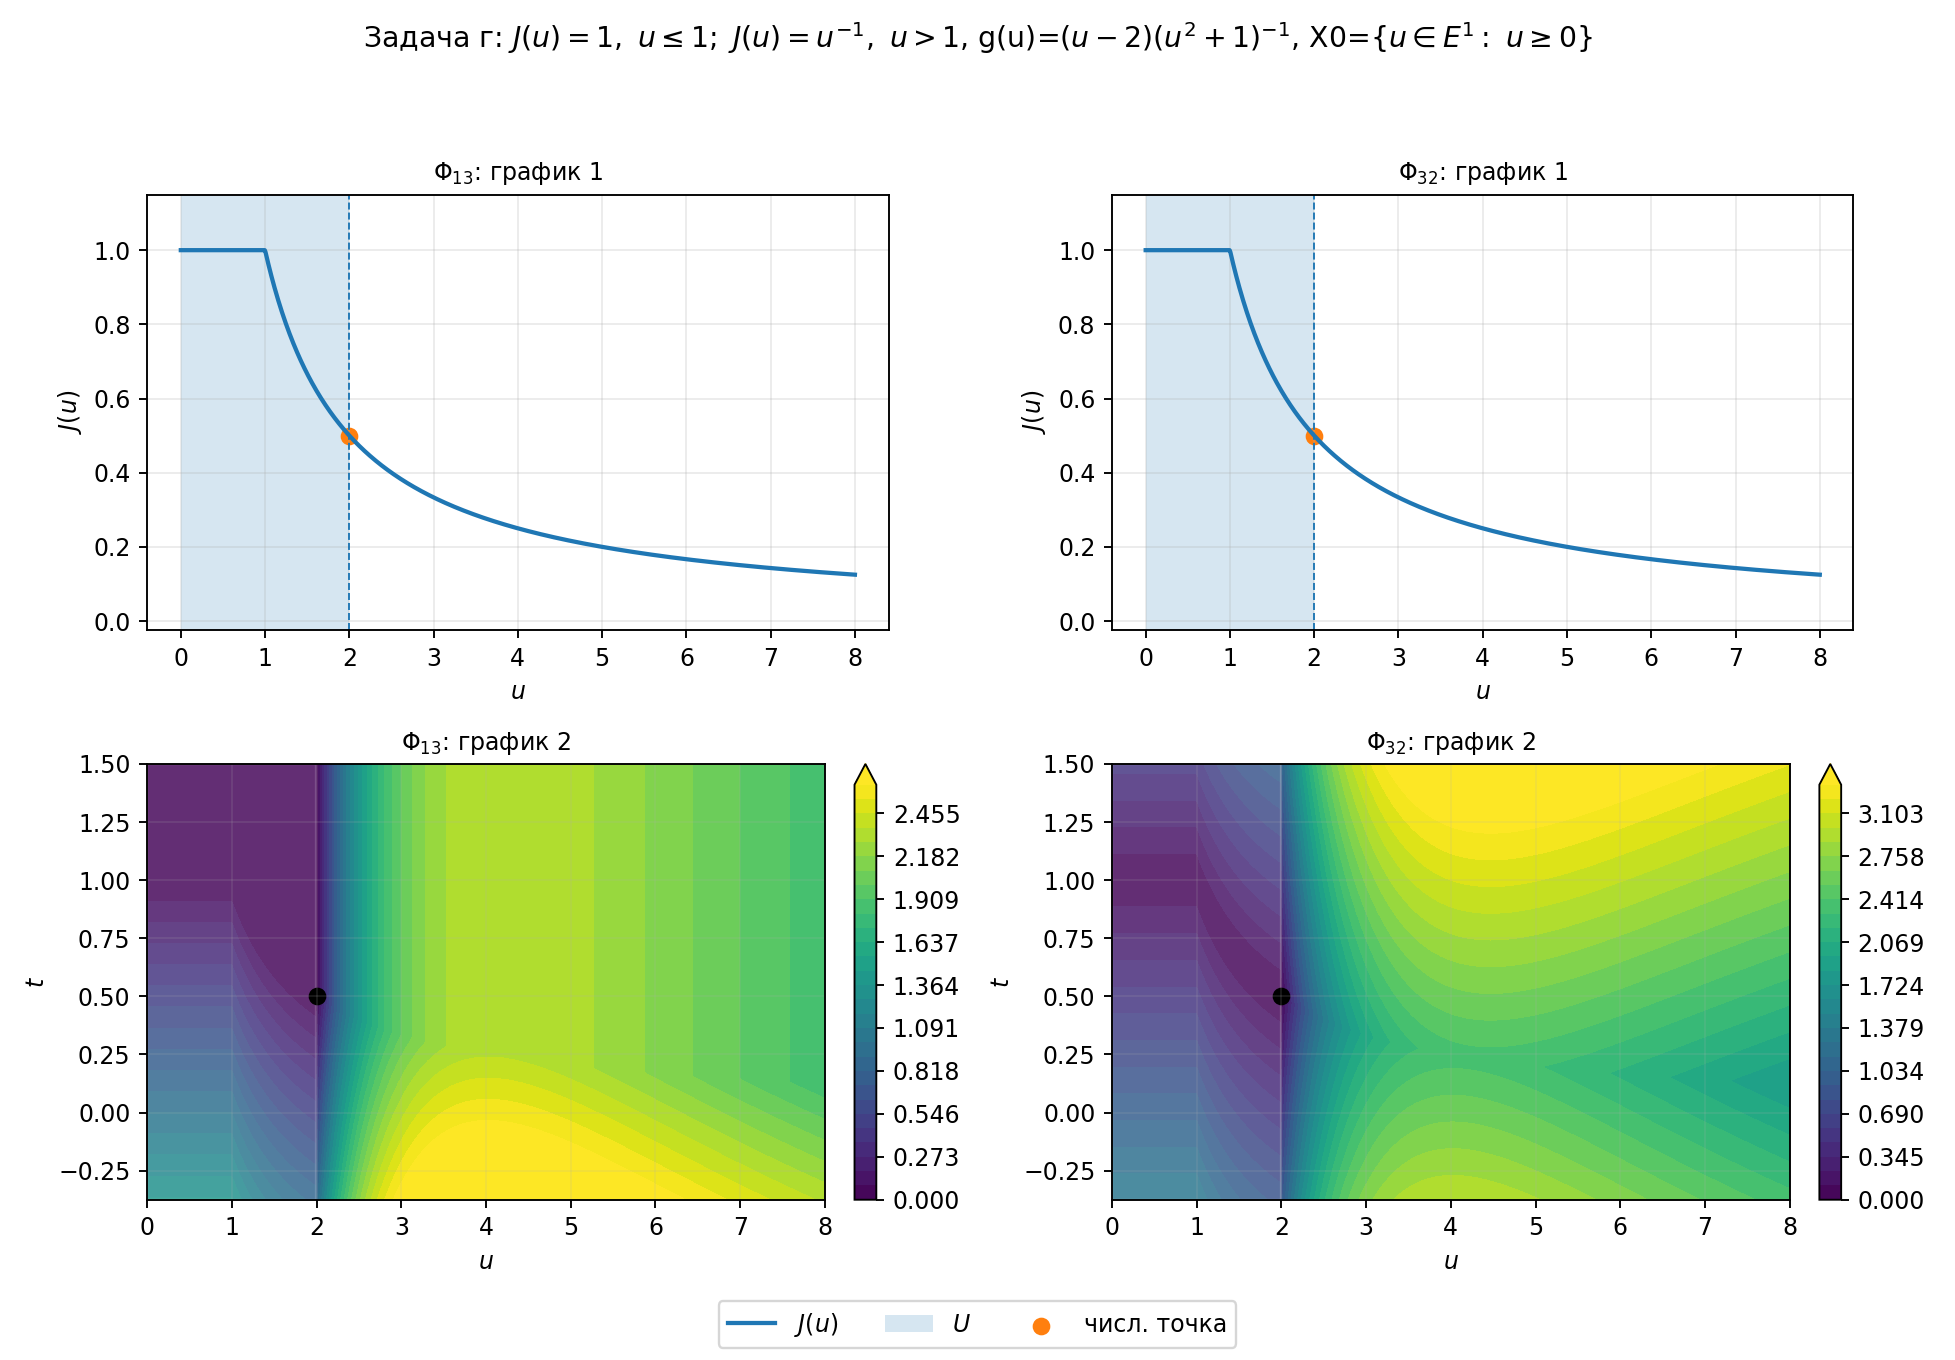
\includegraphics[width=0.96\textwidth]{graphs/g_g2_xge0_overview.png}
\caption{Задача г, вариант g2: $g(u)=(u-2)(u^2+1)^{-1}$, $X_0=\{u\in E^1:\ u\geq 0\}$. Верхний ряд: график 1 для $\Phi_{13}$ и $\Phi_{32}$; нижний ряд: график 2 для $\Phi_{13}$ и $\Phi_{32}$.}
\end{figure}

\begin{figure}[H]
\centering
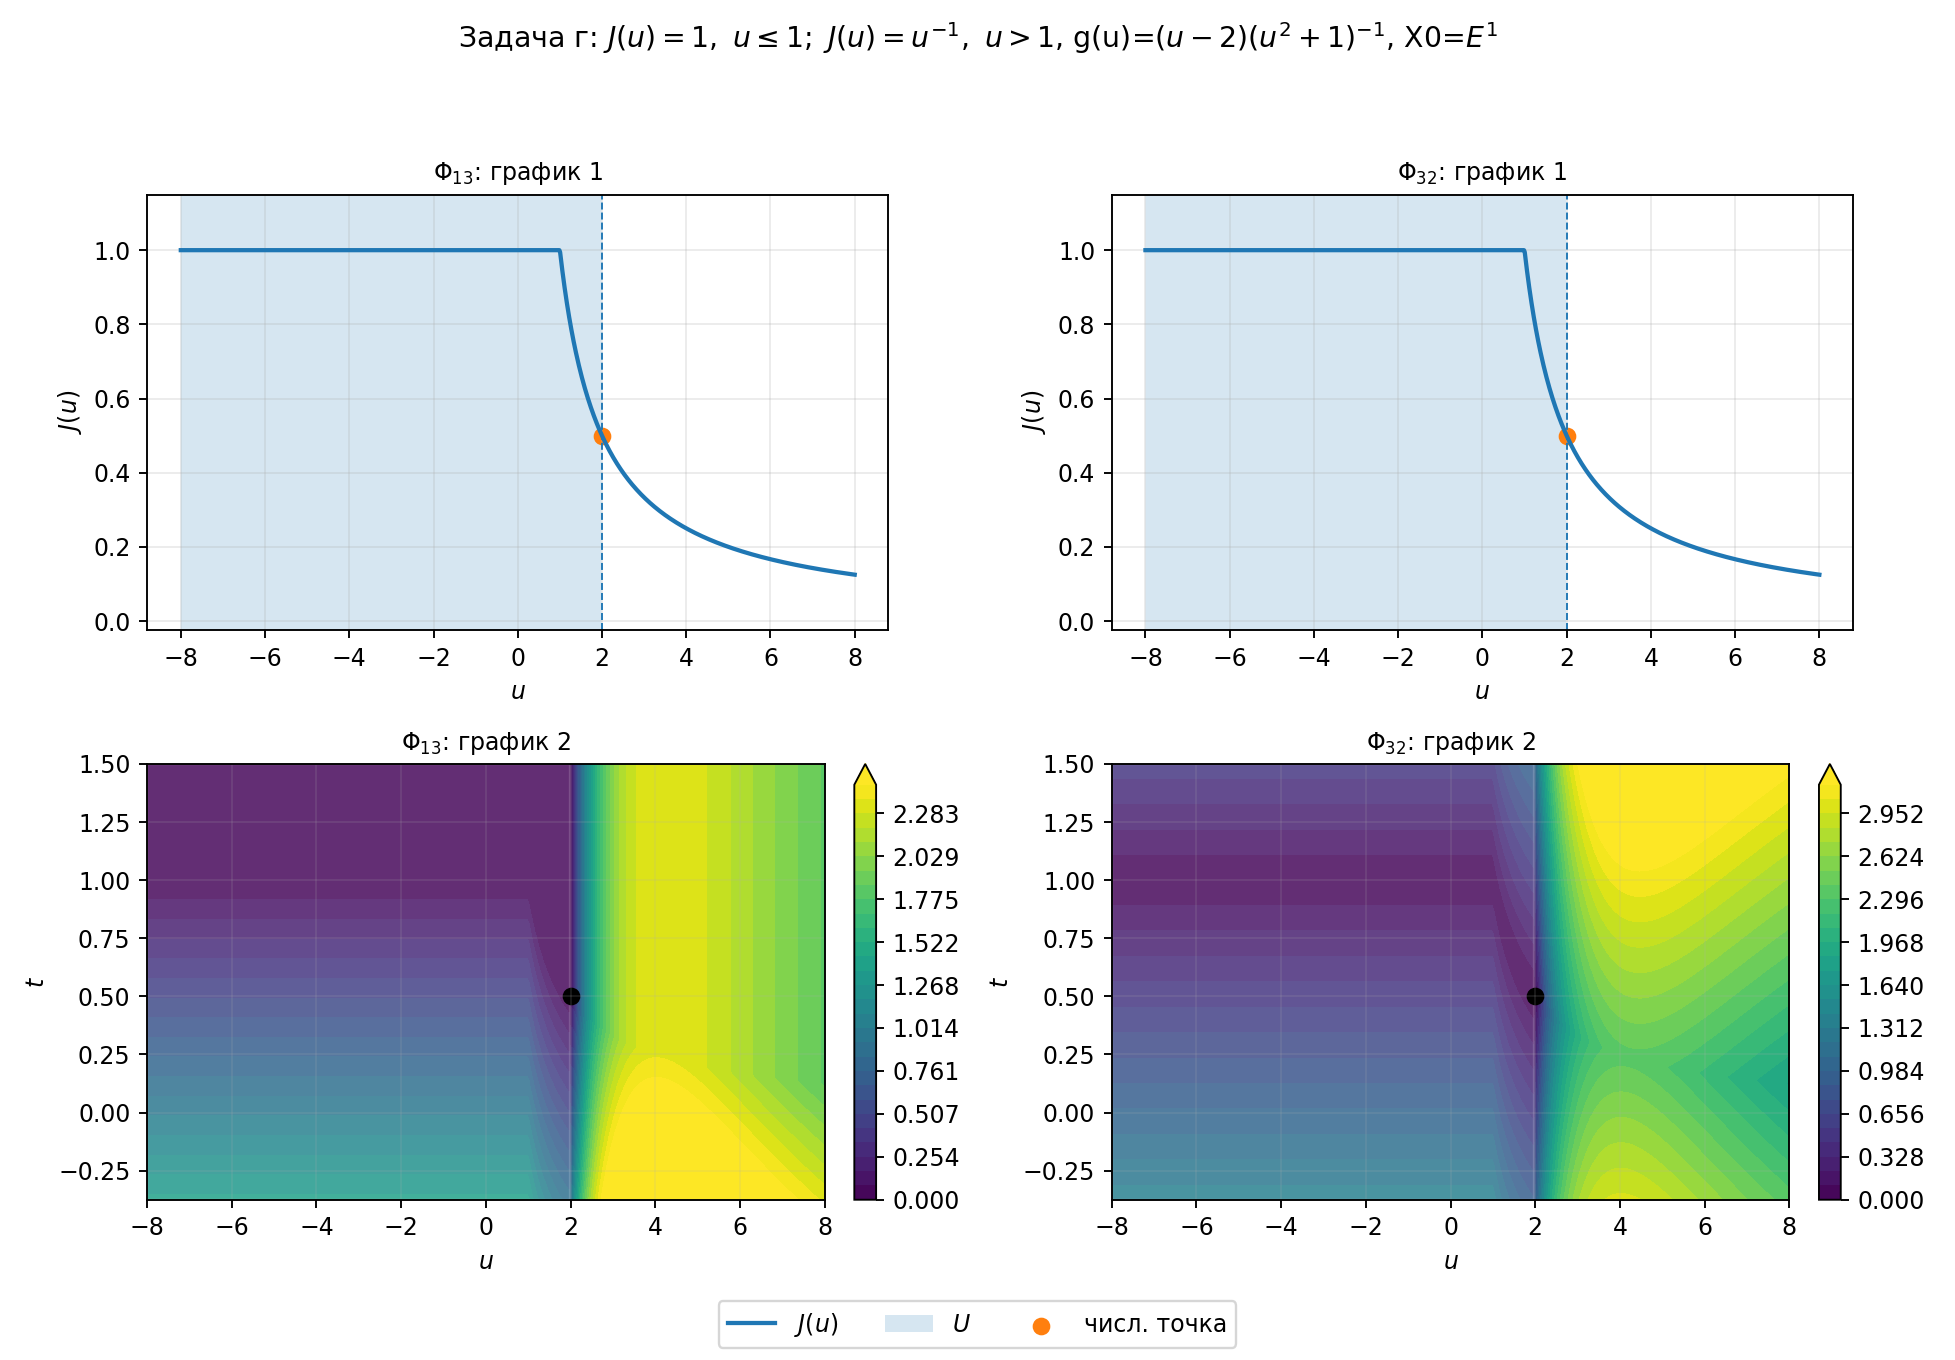
\includegraphics[width=0.96\textwidth]{graphs/g_g2_R_overview.png}
\caption{Задача г, вариант g2: $g(u)=(u-2)(u^2+1)^{-1}$, $X_0=E^1$. Верхний ряд: график 1 для $\Phi_{13}$ и $\Phi_{32}$; нижний ряд: график 2 для $\Phi_{13}$ и $\Phi_{32}$.}
\end{figure}

\begin{figure}[H]
\centering
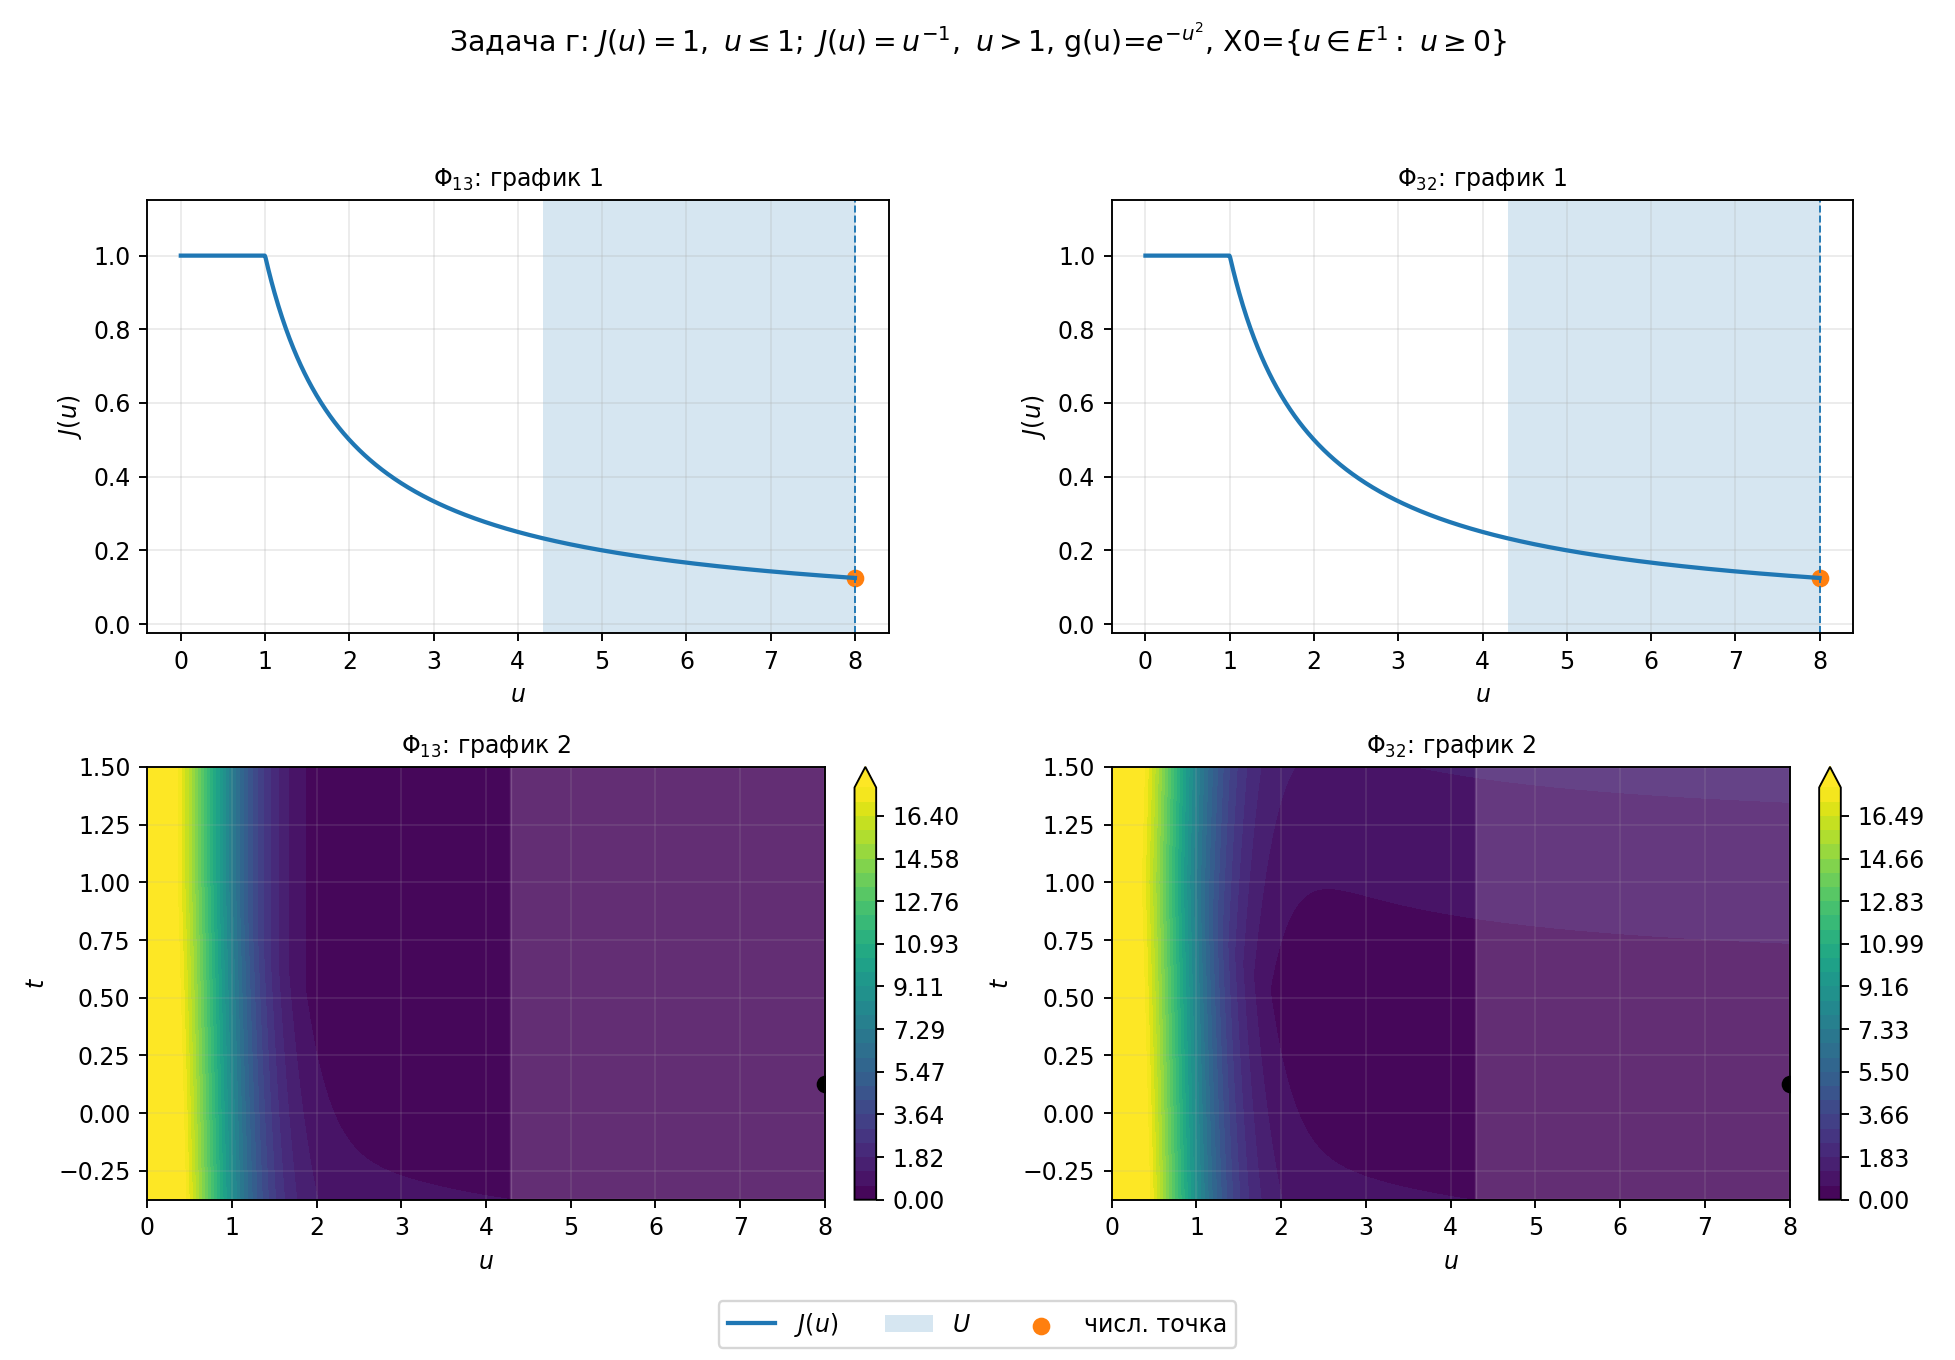
\includegraphics[width=0.96\textwidth]{graphs/g_g3_xge0_overview.png}
\caption{Задача г, вариант g3: $g(u)=e^{-u^2}$, $X_0=\{u\in E^1:\ u\geq 0\}$. Верхний ряд: график 1 для $\Phi_{13}$ и $\Phi_{32}$; нижний ряд: график 2 для $\Phi_{13}$ и $\Phi_{32}$.}
\end{figure}

\begin{figure}[H]
\centering
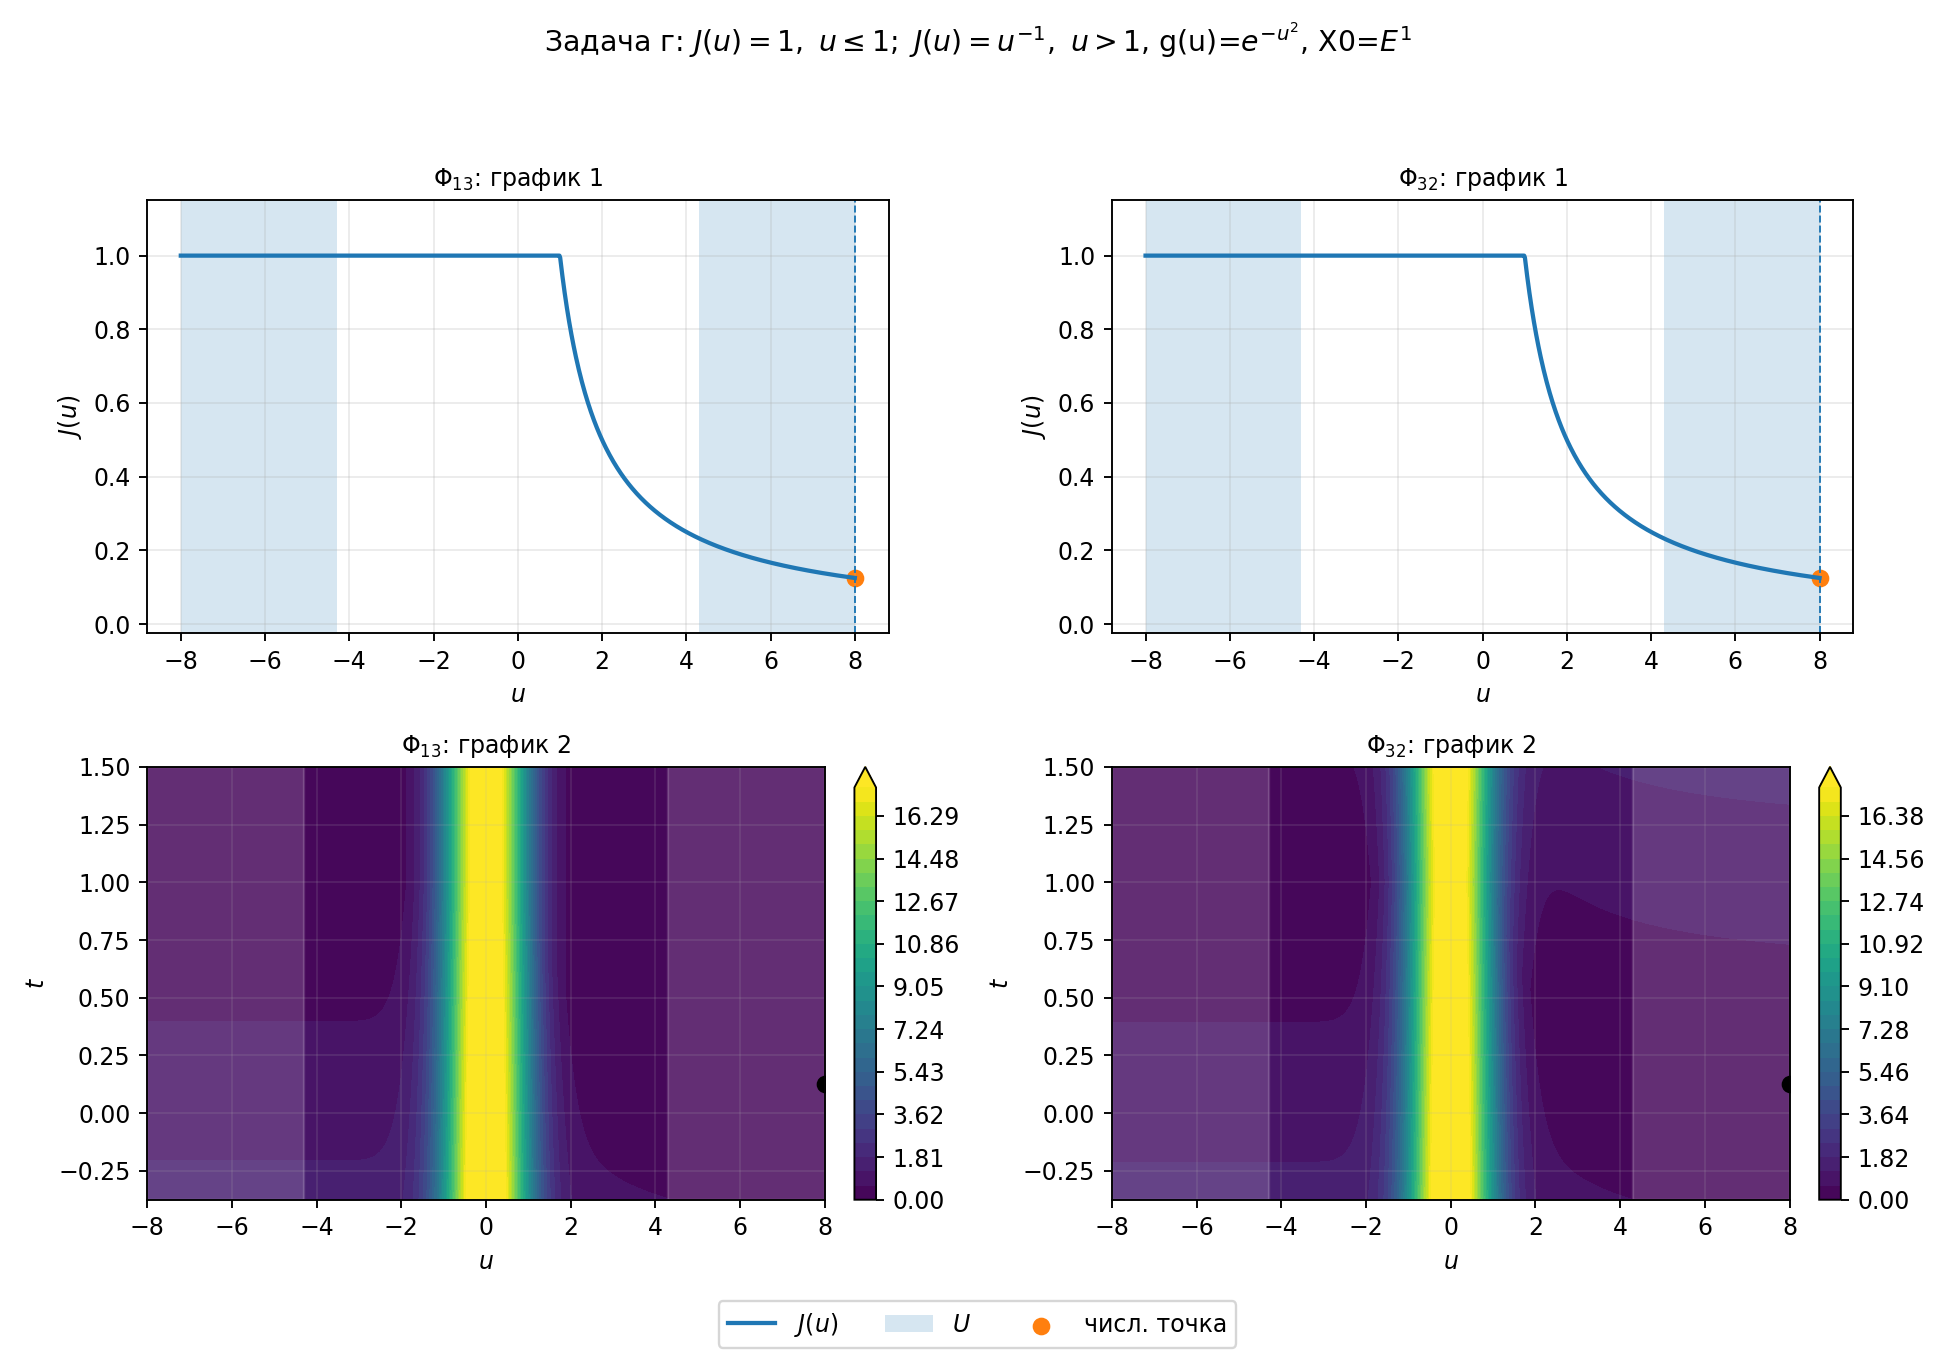
\includegraphics[width=0.96\textwidth]{graphs/g_g3_R_overview.png}
\caption{Задача г, вариант g3: $g(u)=e^{-u^2}$, $X_0=E^1$. Верхний ряд: график 1 для $\Phi_{13}$ и $\Phi_{32}$; нижний ряд: график 2 для $\Phi_{13}$ и $\Phi_{32}$.}
\end{figure}

\begin{figure}[H]
\centering
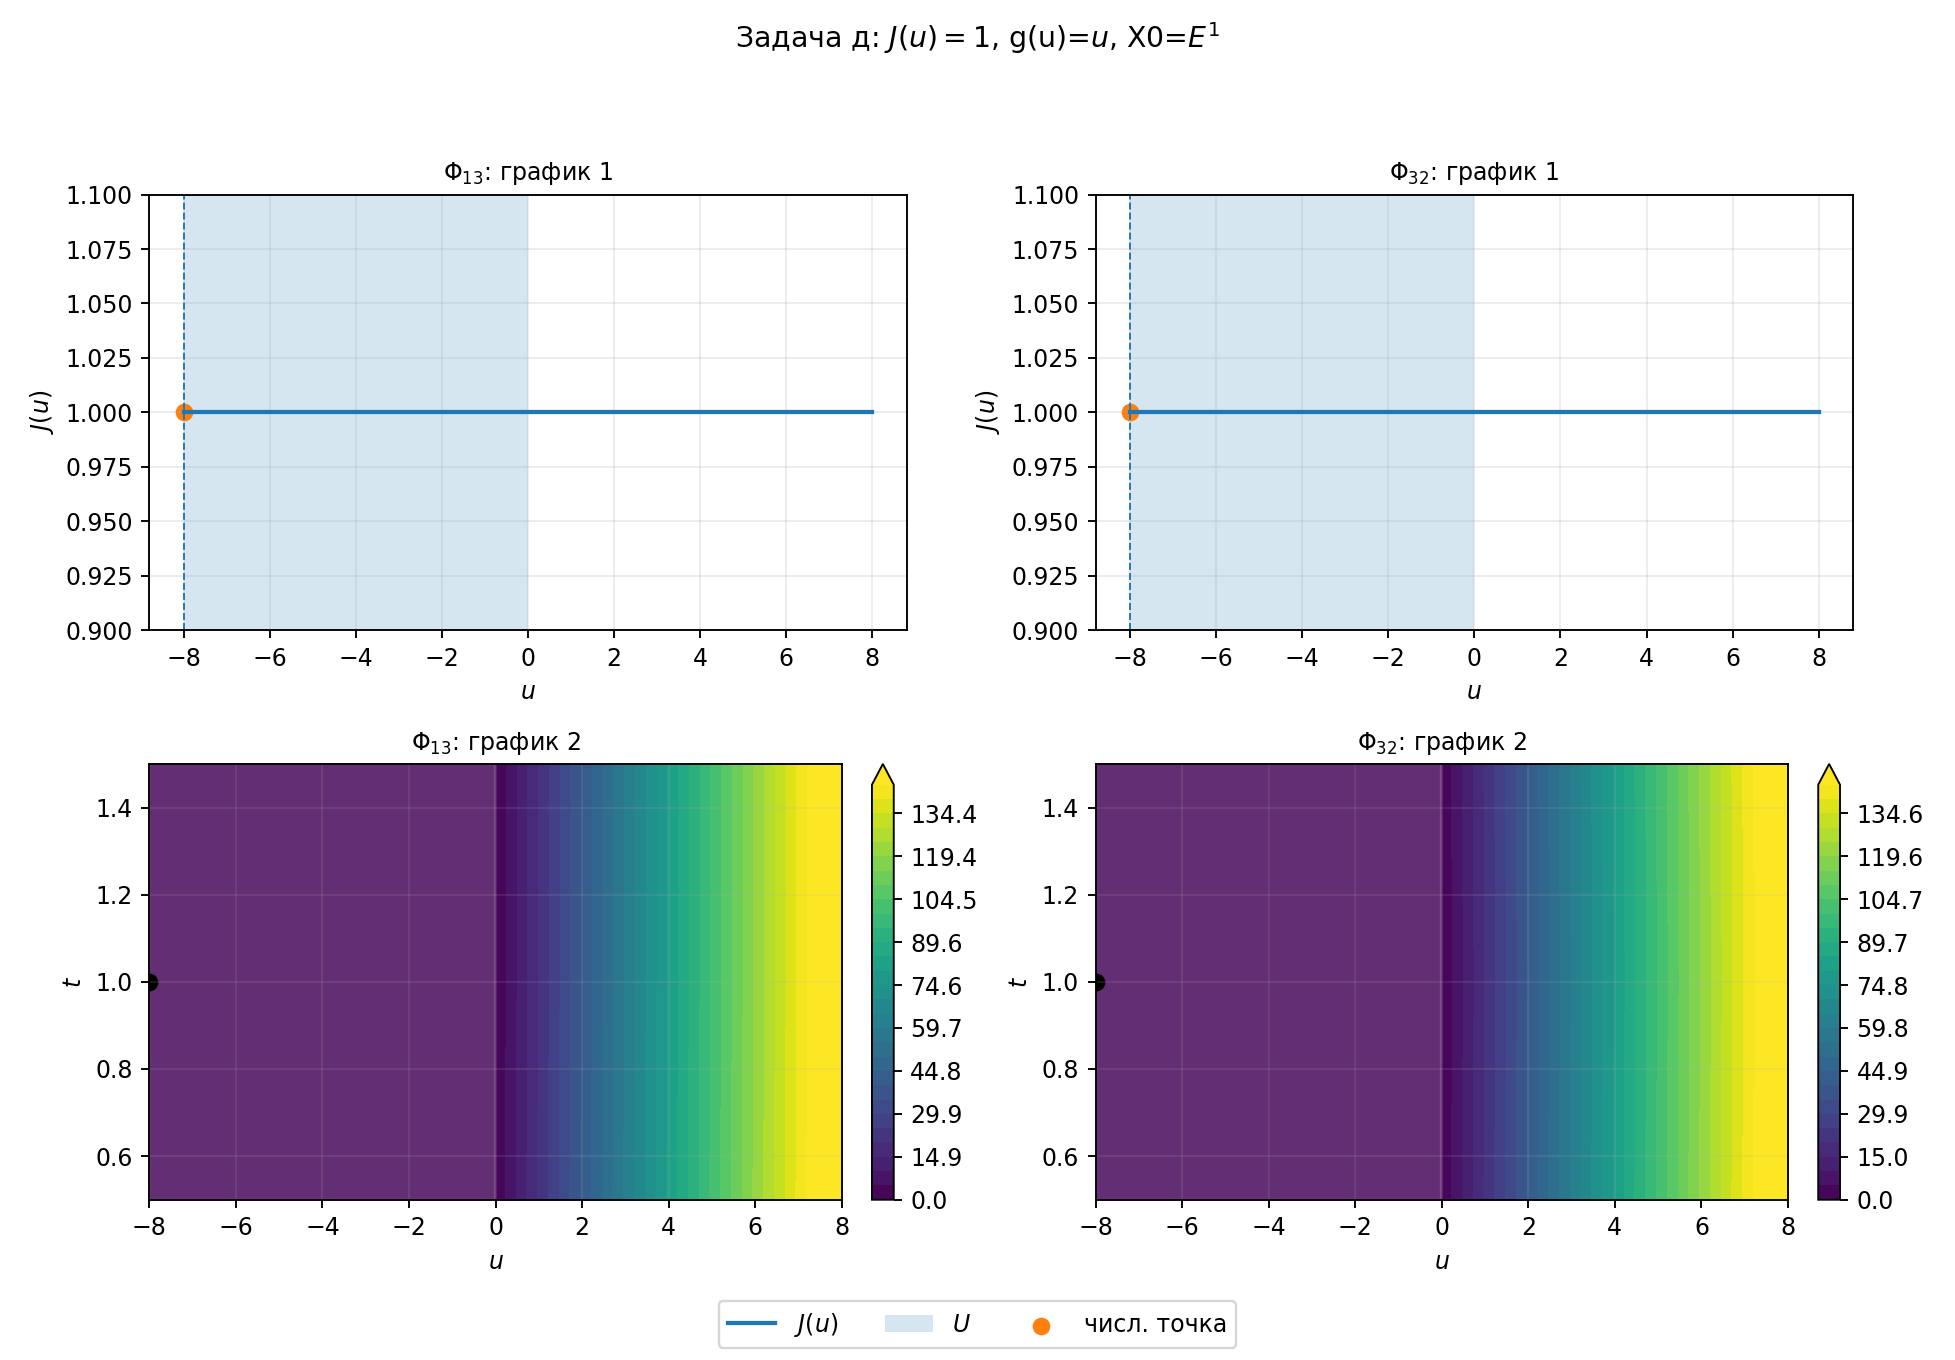
\includegraphics[width=0.96\textwidth]{graphs/d_g1_R_overview.png}
\caption{Задача д, вариант g1: $g(u)=u$, $X_0=E^1$. Верхний ряд: график 1 для $\Phi_{13}$ и $\Phi_{32}$; нижний ряд: график 2 для $\Phi_{13}$ и $\Phi_{32}$.}
\end{figure}

\begin{figure}[H]
\centering
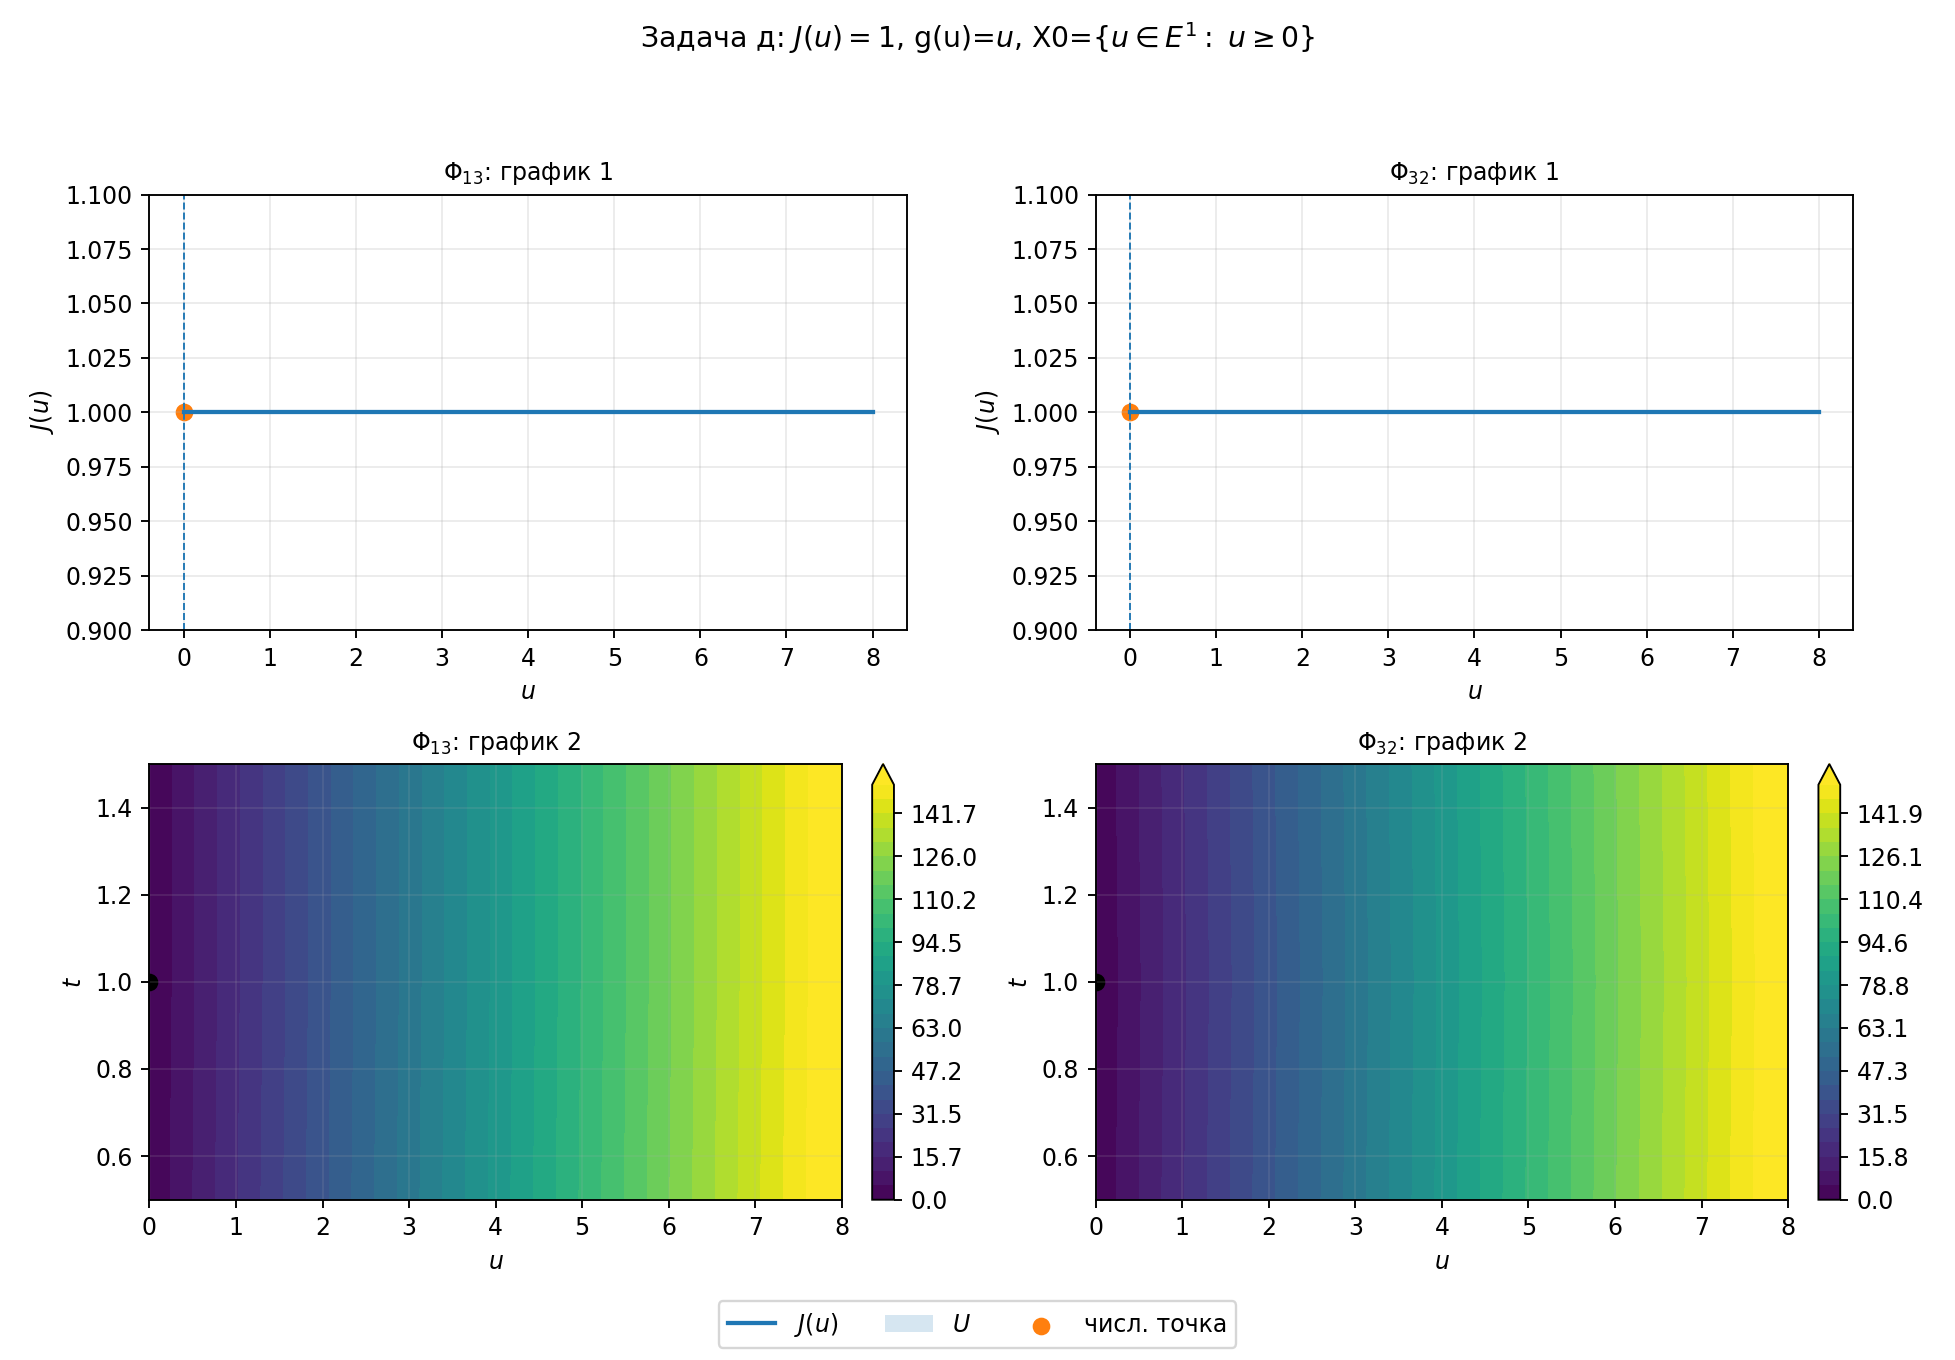
\includegraphics[width=0.96\textwidth]{graphs/d_g1_xge0_overview.png}
\caption{Задача д, вариант g1: $g(u)=u$, $X_0=\{u\in E^1:\ u\geq 0\}$. Верхний ряд: график 1 для $\Phi_{13}$ и $\Phi_{32}$; нижний ряд: график 2 для $\Phi_{13}$ и $\Phi_{32}$.}
\end{figure}

\begin{figure}[H]
\centering
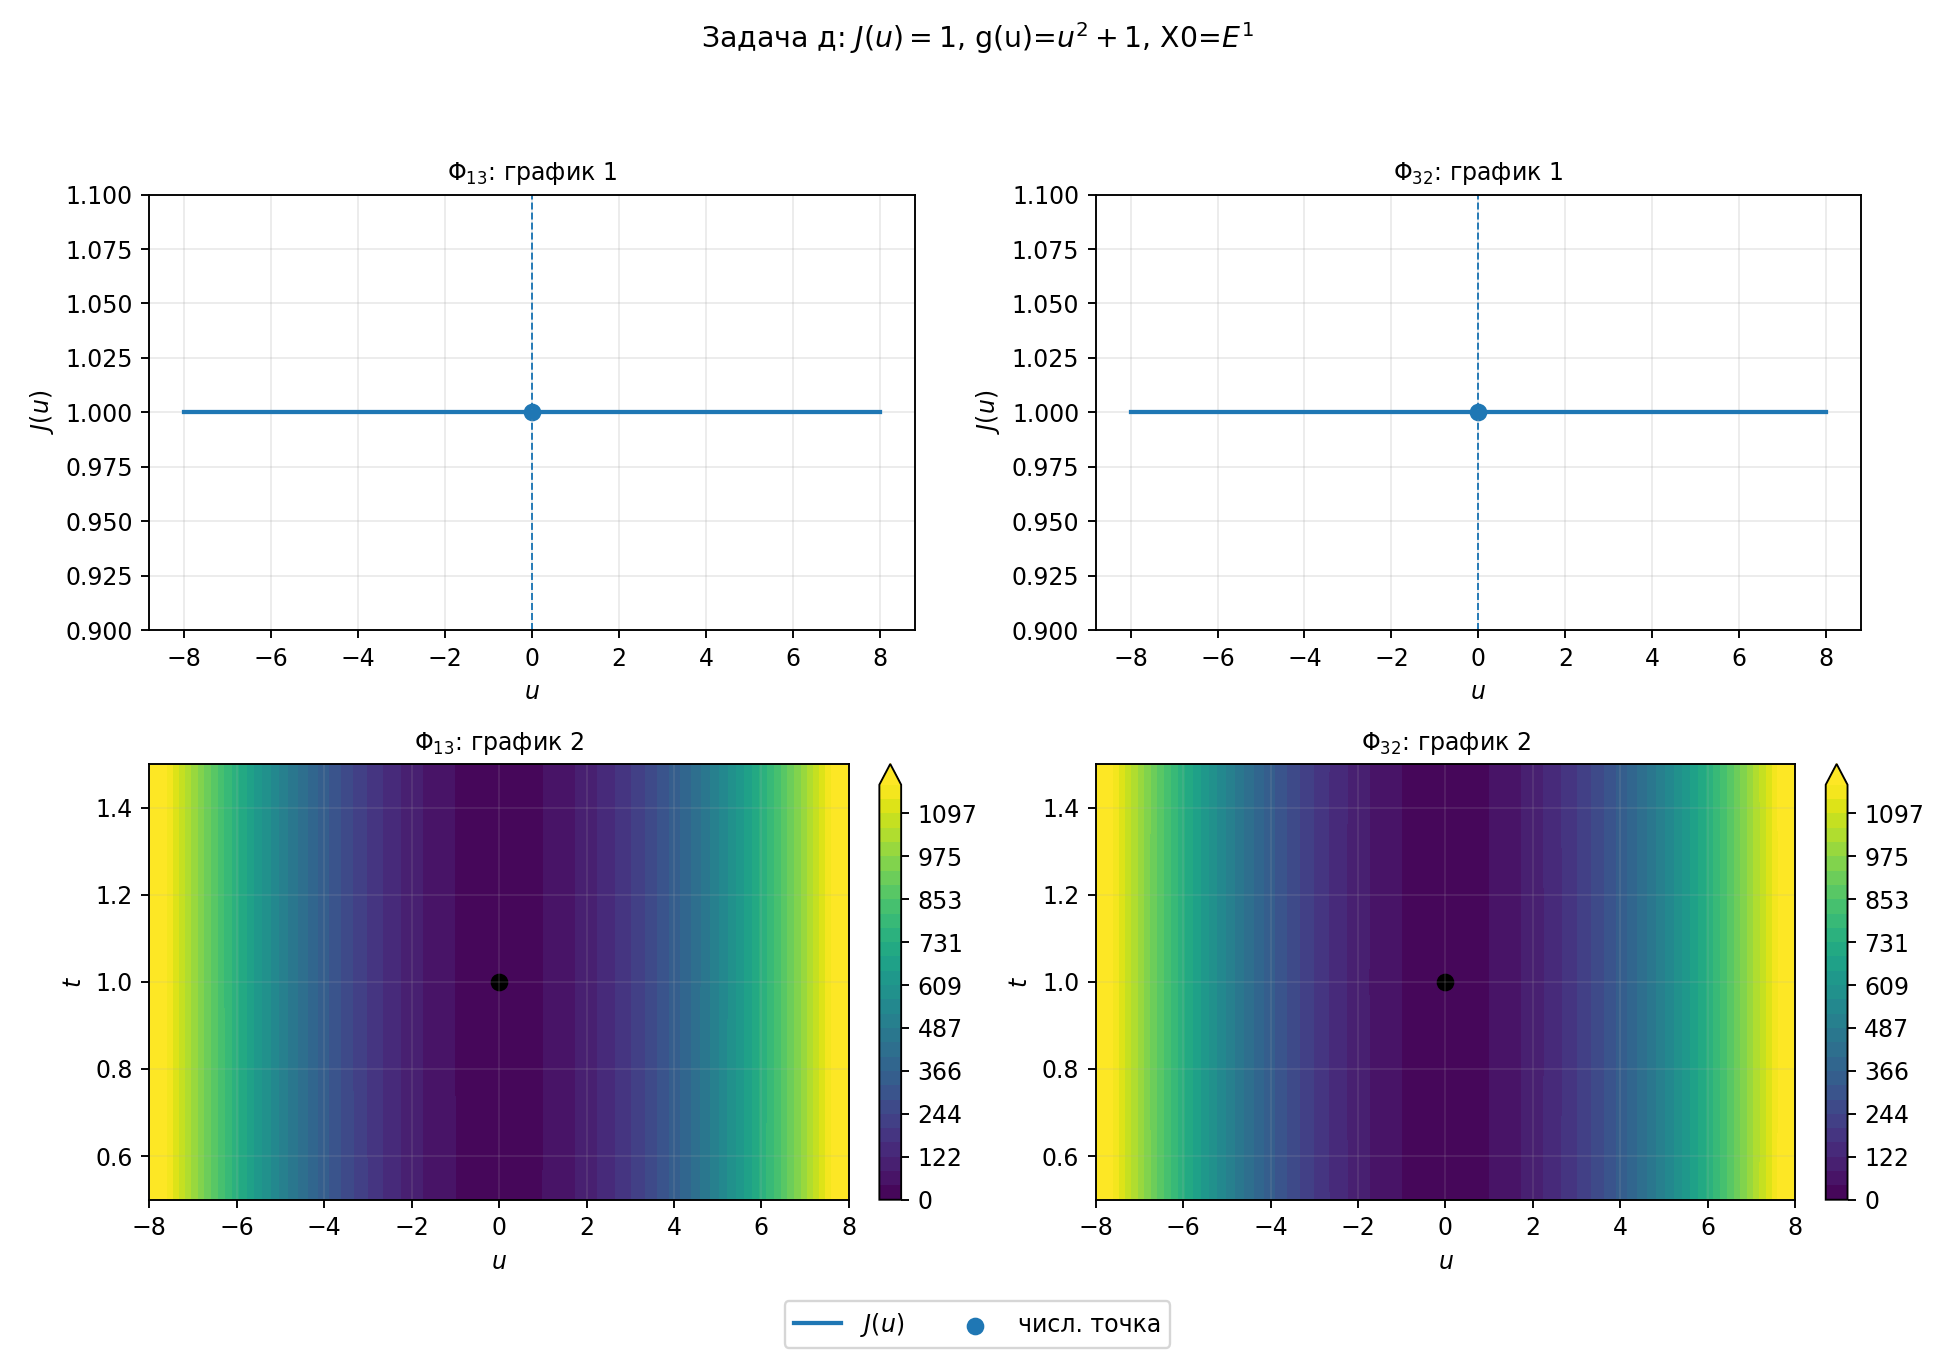
\includegraphics[width=0.96\textwidth]{graphs/d_g2_R_overview.png}
\caption{Задача д, вариант g2: $g(u)=u^2+1$, $X_0=E^1$. Верхний ряд: график 1 для $\Phi_{13}$ и $\Phi_{32}$; нижний ряд: график 2 для $\Phi_{13}$ и $\Phi_{32}$.}
\end{figure}

\begin{figure}[H]
\centering
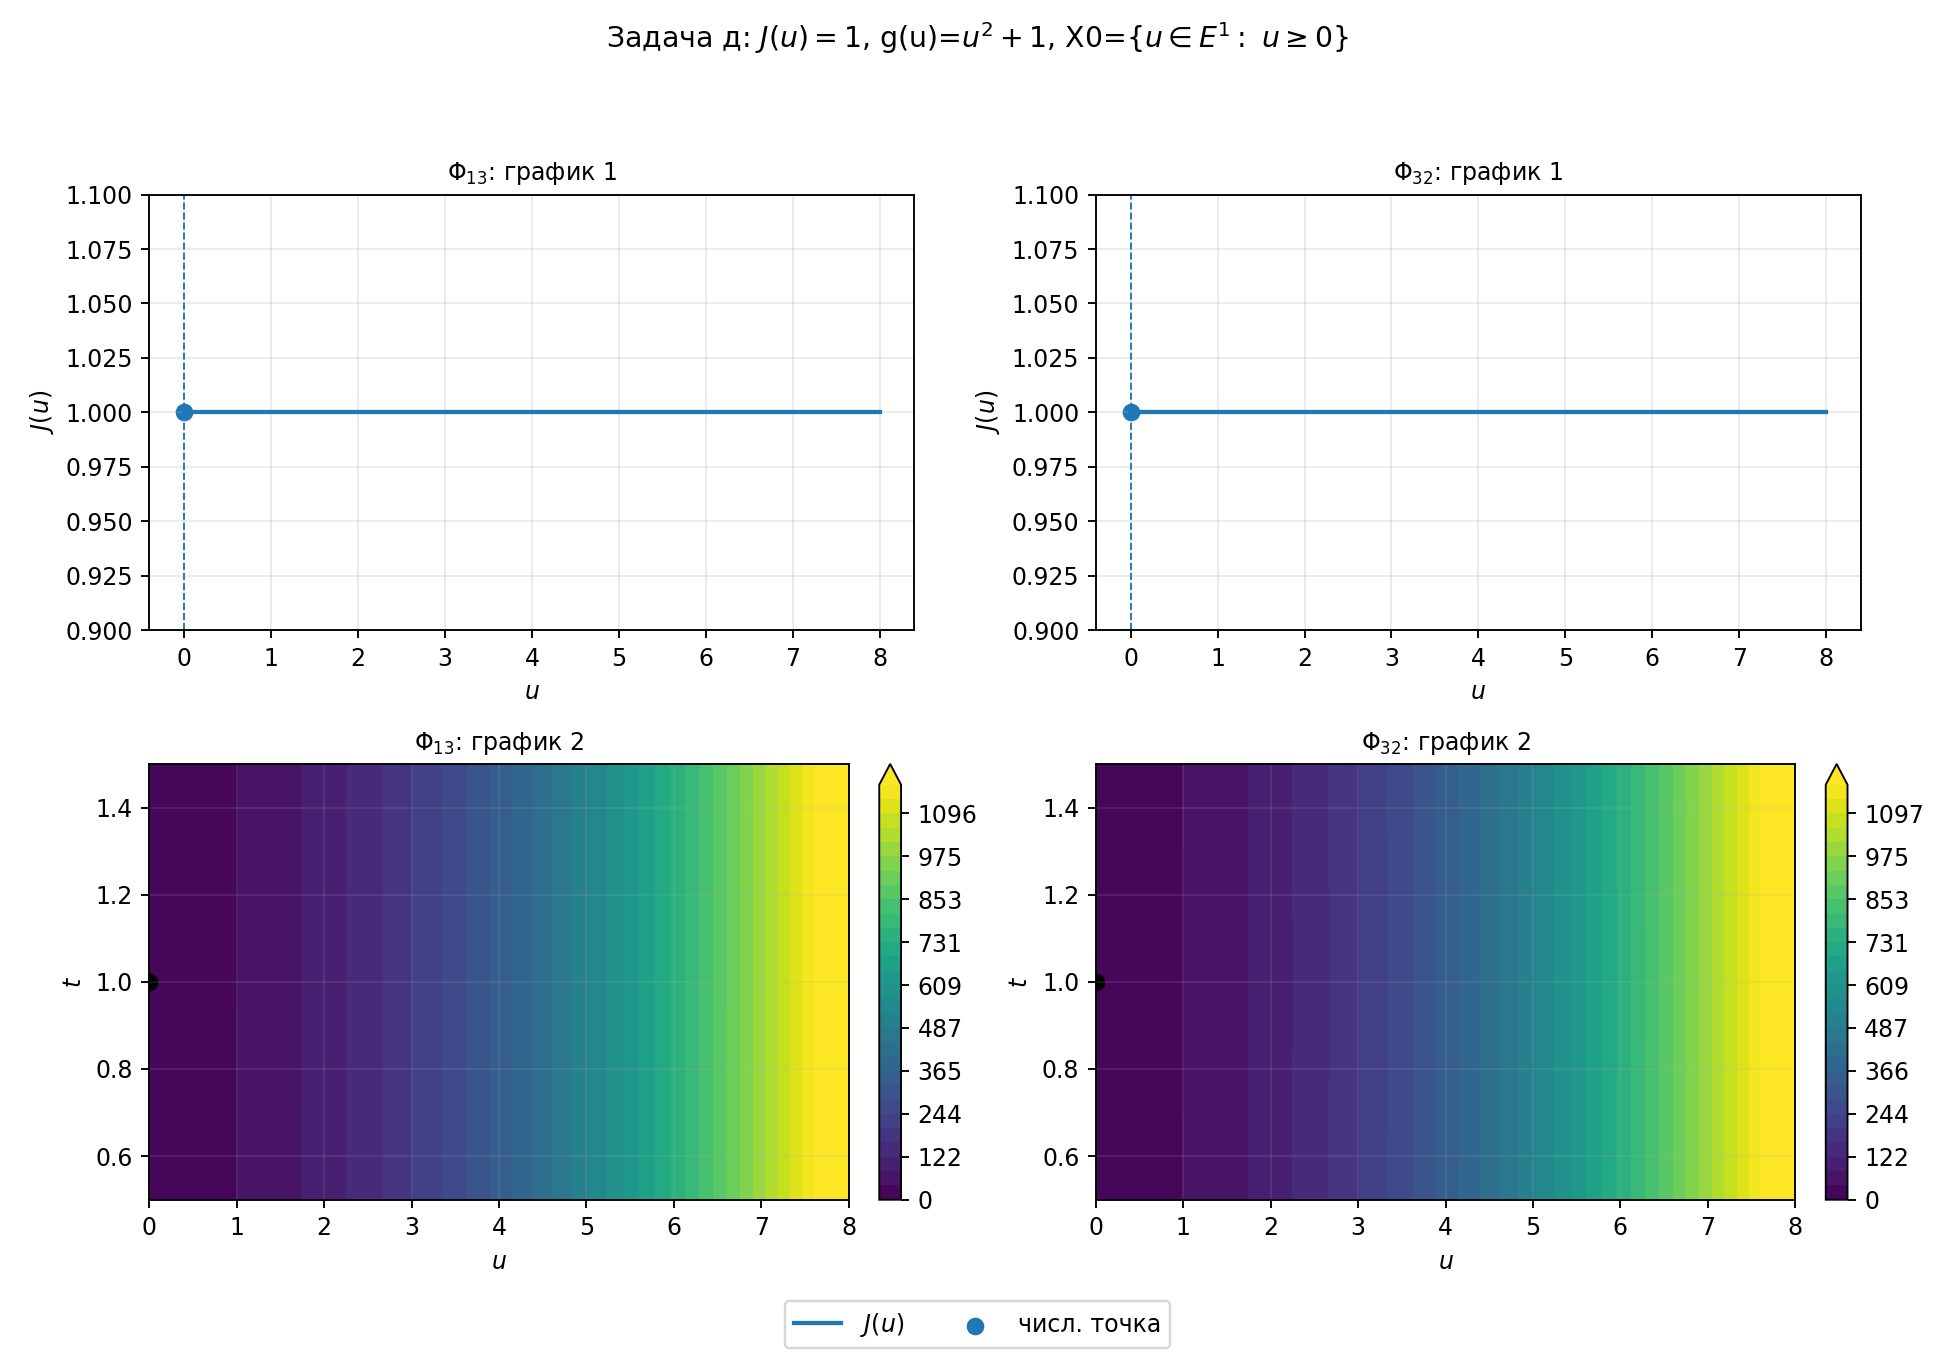
\includegraphics[width=0.96\textwidth]{graphs/d_g2_xge0_overview.png}
\caption{Задача д, вариант g2: $g(u)=u^2+1$, $X_0=\{u\in E^1:\ u\geq 0\}$. Верхний ряд: график 1 для $\Phi_{13}$ и $\Phi_{32}$; нижний ряд: график 2 для $\Phi_{13}$ и $\Phi_{32}$.}
\end{figure}

\begin{figure}[H]
\centering
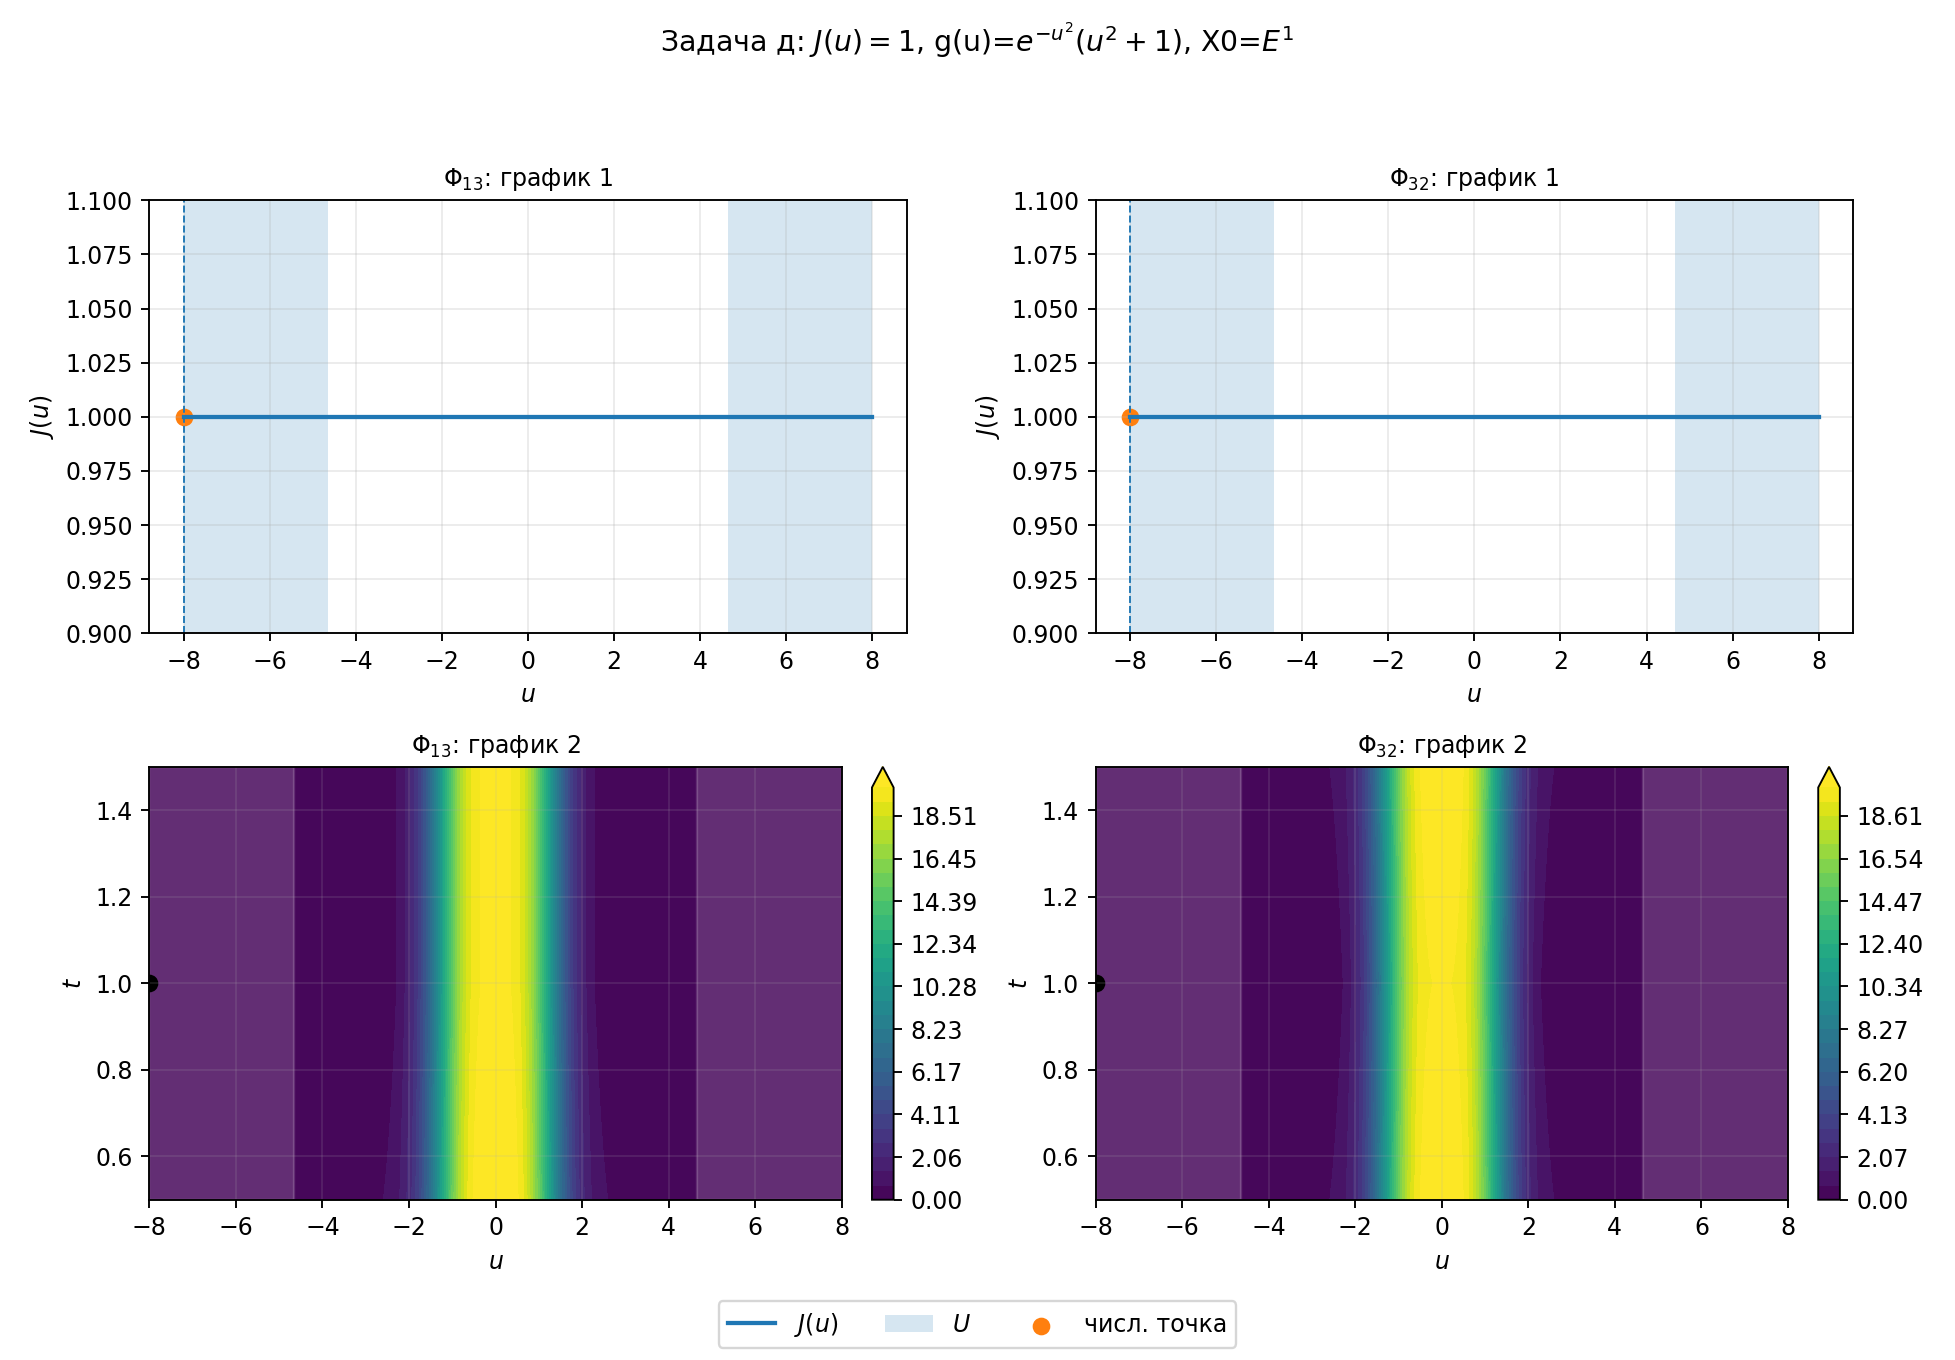
\includegraphics[width=0.96\textwidth]{graphs/d_g3_R_overview.png}
\caption{Задача д, вариант g3: $g(u)=e^{-u^2}(u^2+1)$, $X_0=E^1$. Верхний ряд: график 1 для $\Phi_{13}$ и $\Phi_{32}$; нижний ряд: график 2 для $\Phi_{13}$ и $\Phi_{32}$.}
\end{figure}

\begin{figure}[H]
\centering
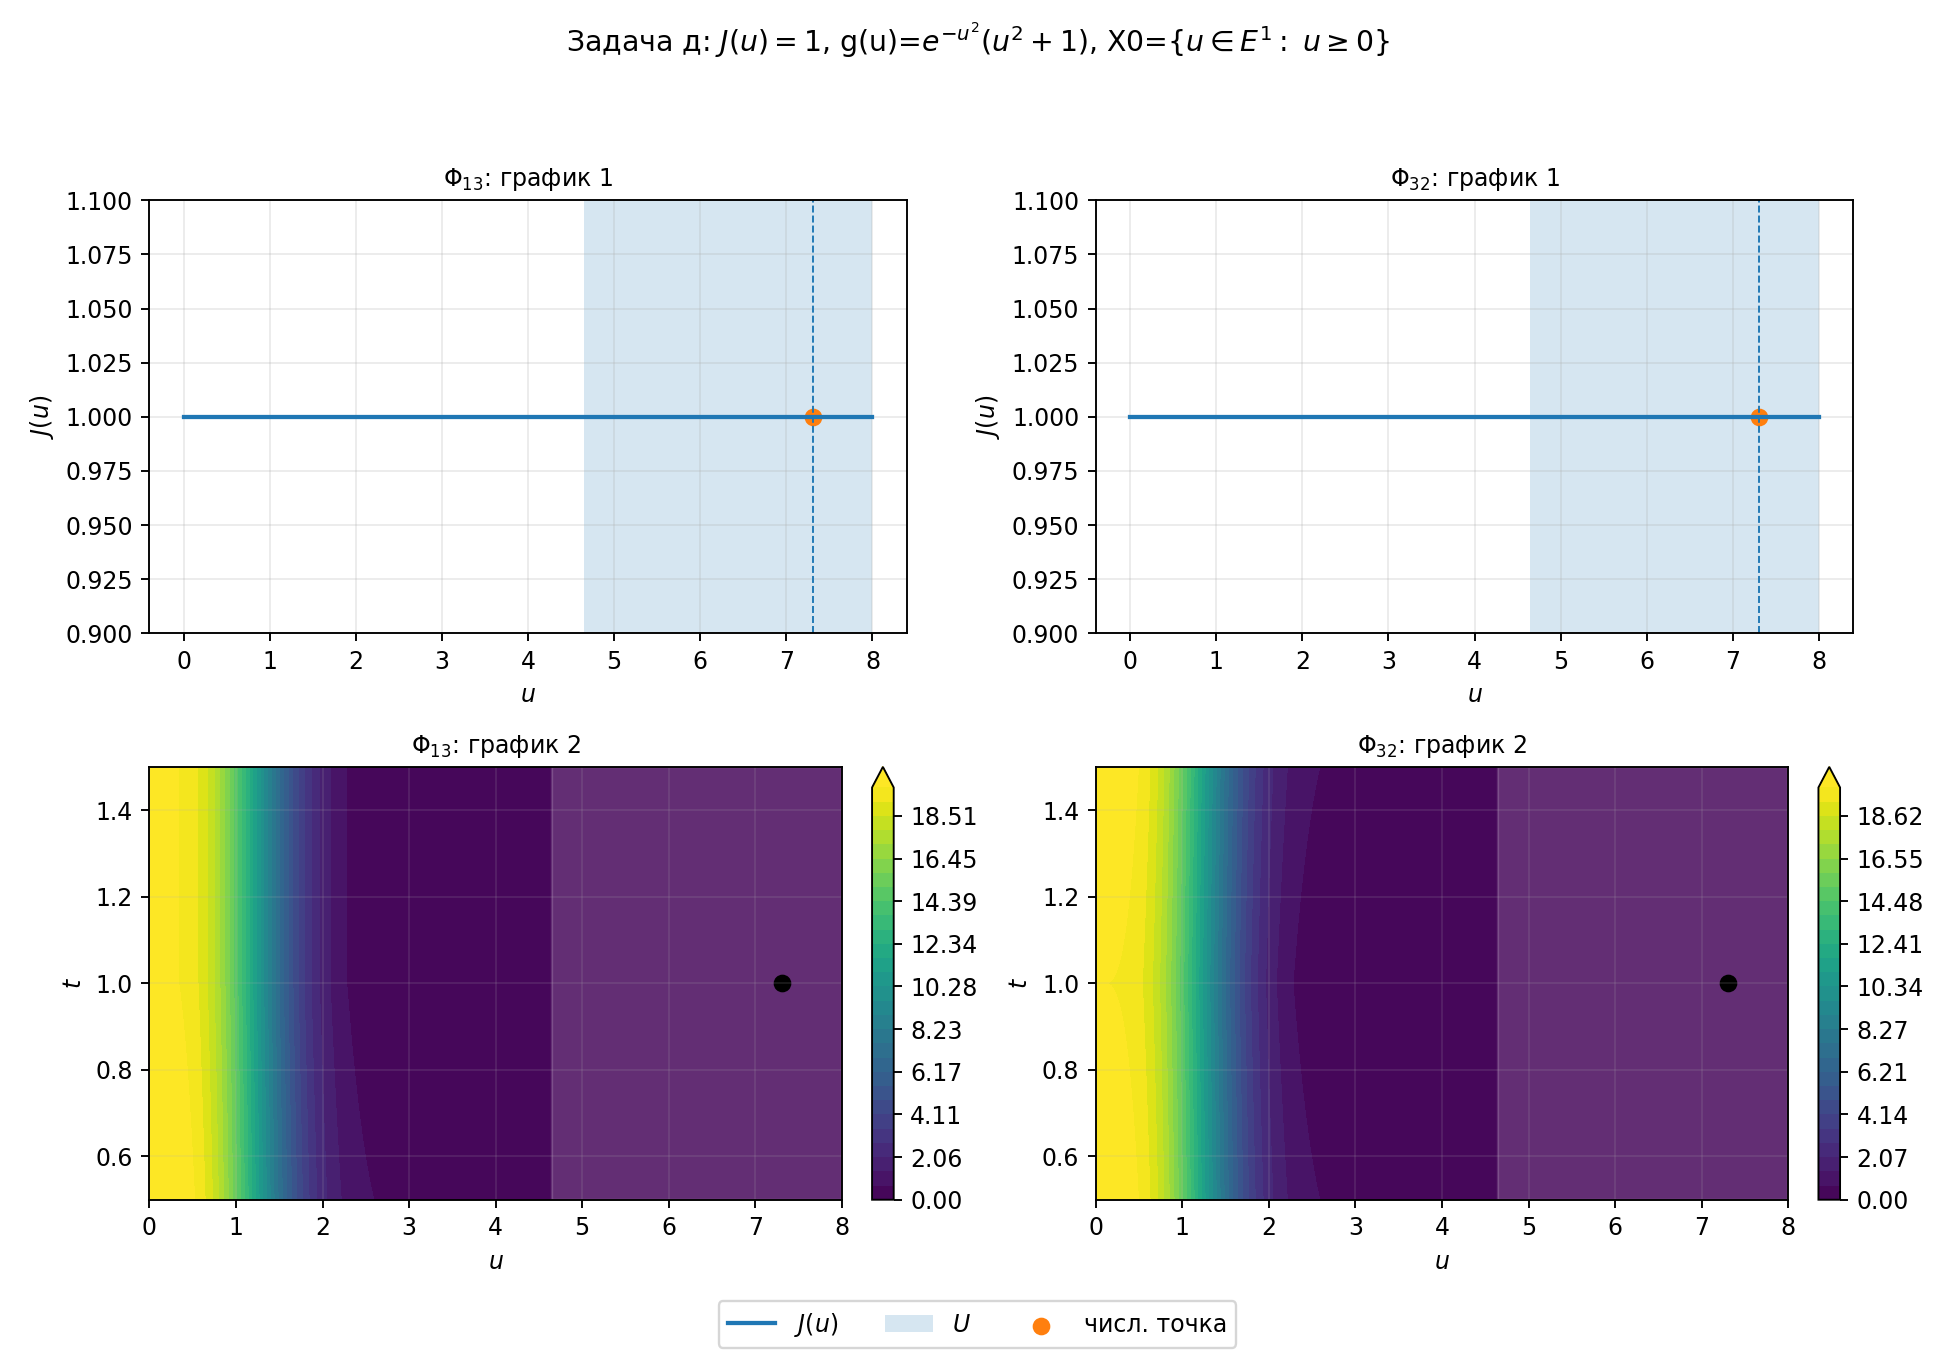
\includegraphics[width=0.96\textwidth]{graphs/d_g3_xge0_overview.png}
\caption{Задача д, вариант g3: $g(u)=e^{-u^2}(u^2+1)$, $X_0=\{u\in E^1:\ u\geq 0\}$. Верхний ряд: график 1 для $\Phi_{13}$ и $\Phi_{32}$; нижний ряд: график 2 для $\Phi_{13}$ и $\Phi_{32}$.}
\end{figure}

\begin{figure}[H]
\centering
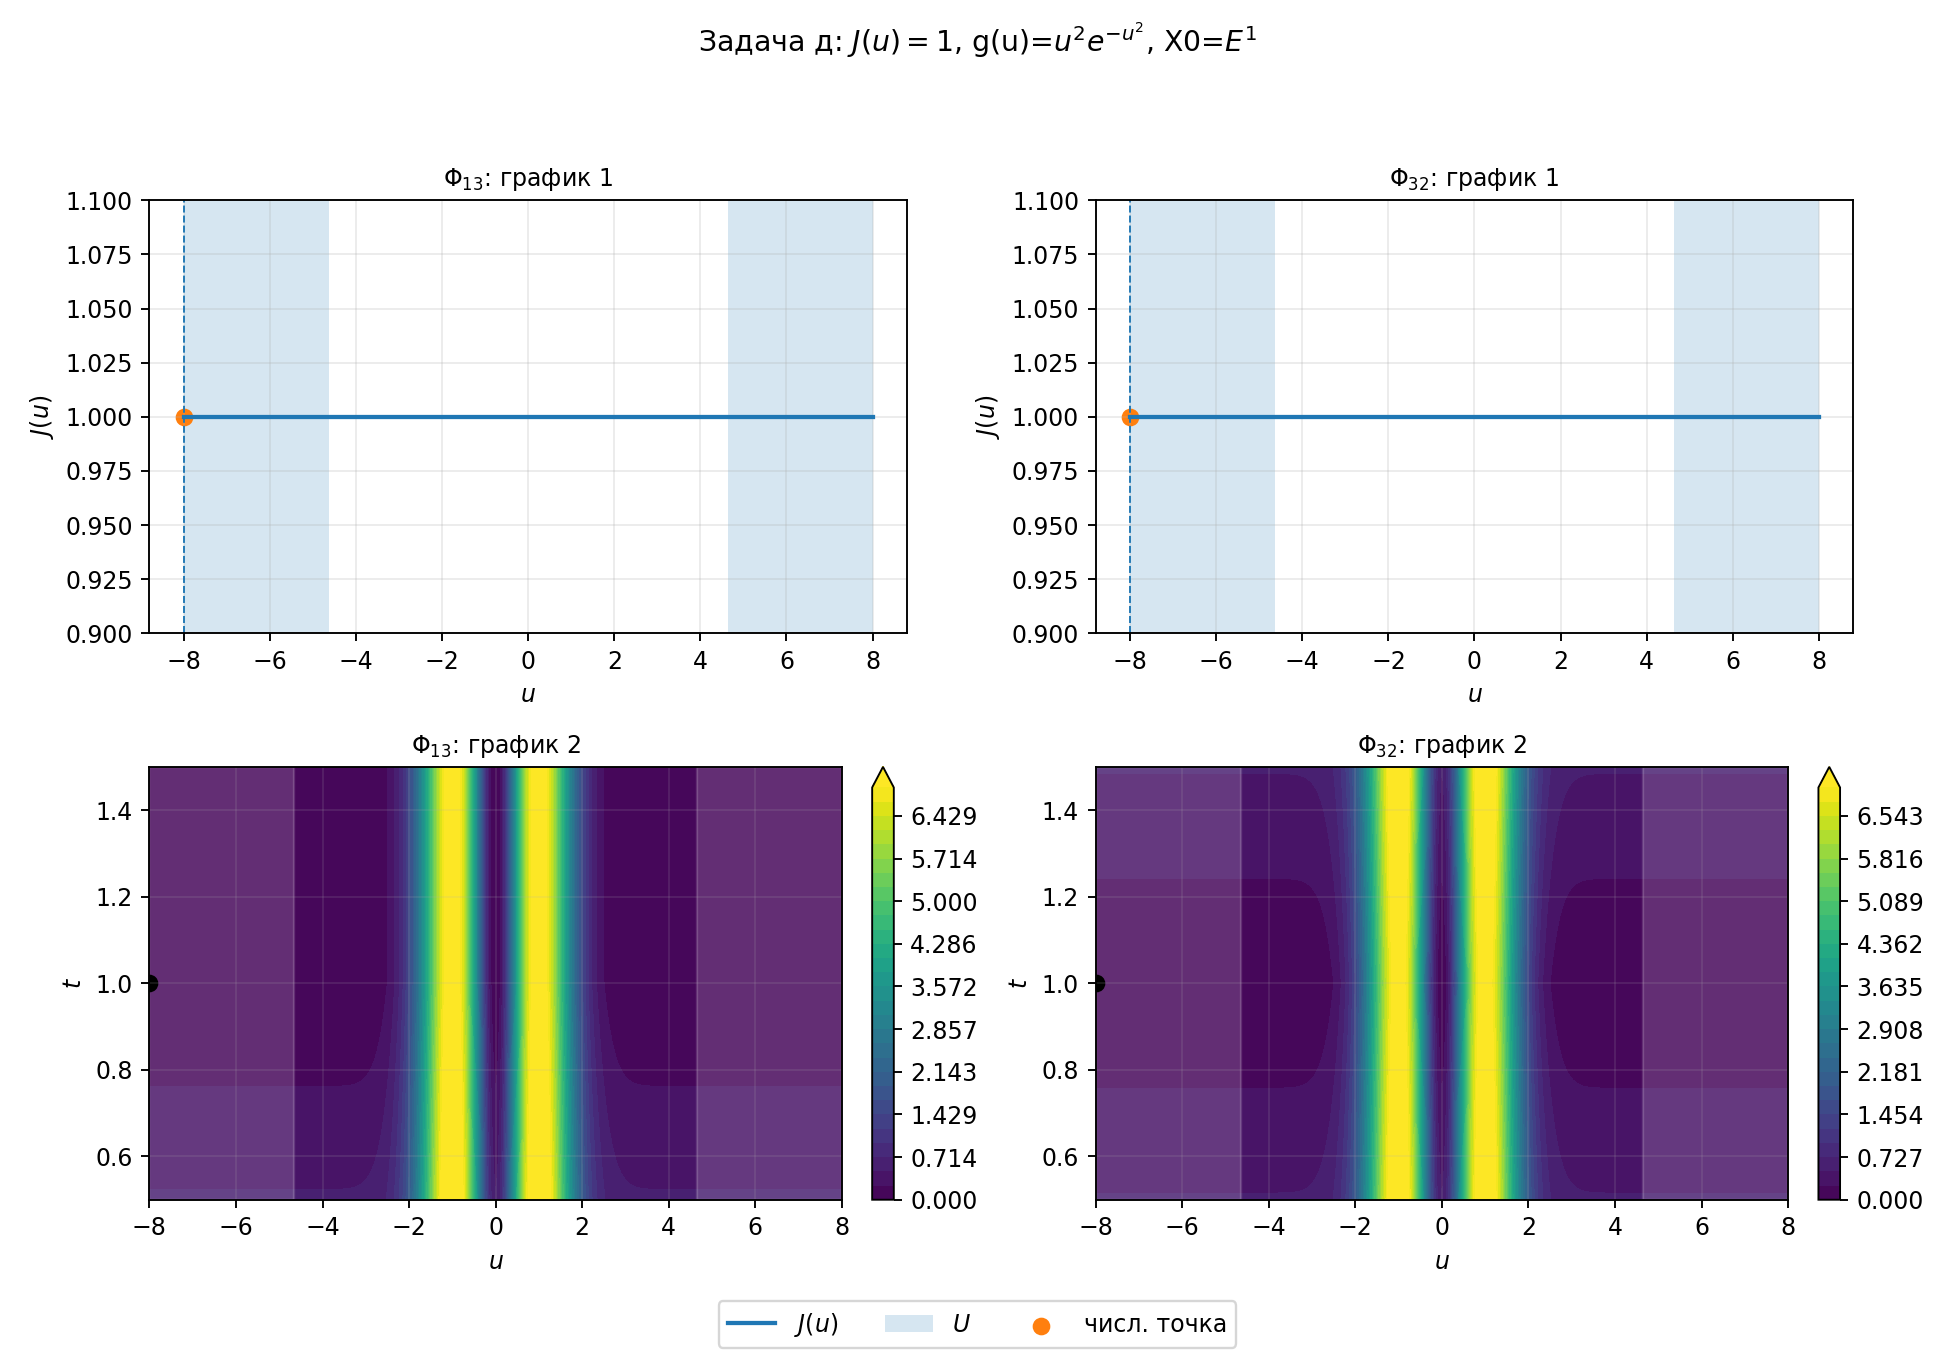
\includegraphics[width=0.96\textwidth]{graphs/d_g4_R_overview.png}
\caption{Задача д, вариант g4: $g(u)=u^2e^{-u^2}$, $X_0=E^1$. Верхний ряд: график 1 для $\Phi_{13}$ и $\Phi_{32}$; нижний ряд: график 2 для $\Phi_{13}$ и $\Phi_{32}$.}
\end{figure}

\begin{figure}[H]
\centering
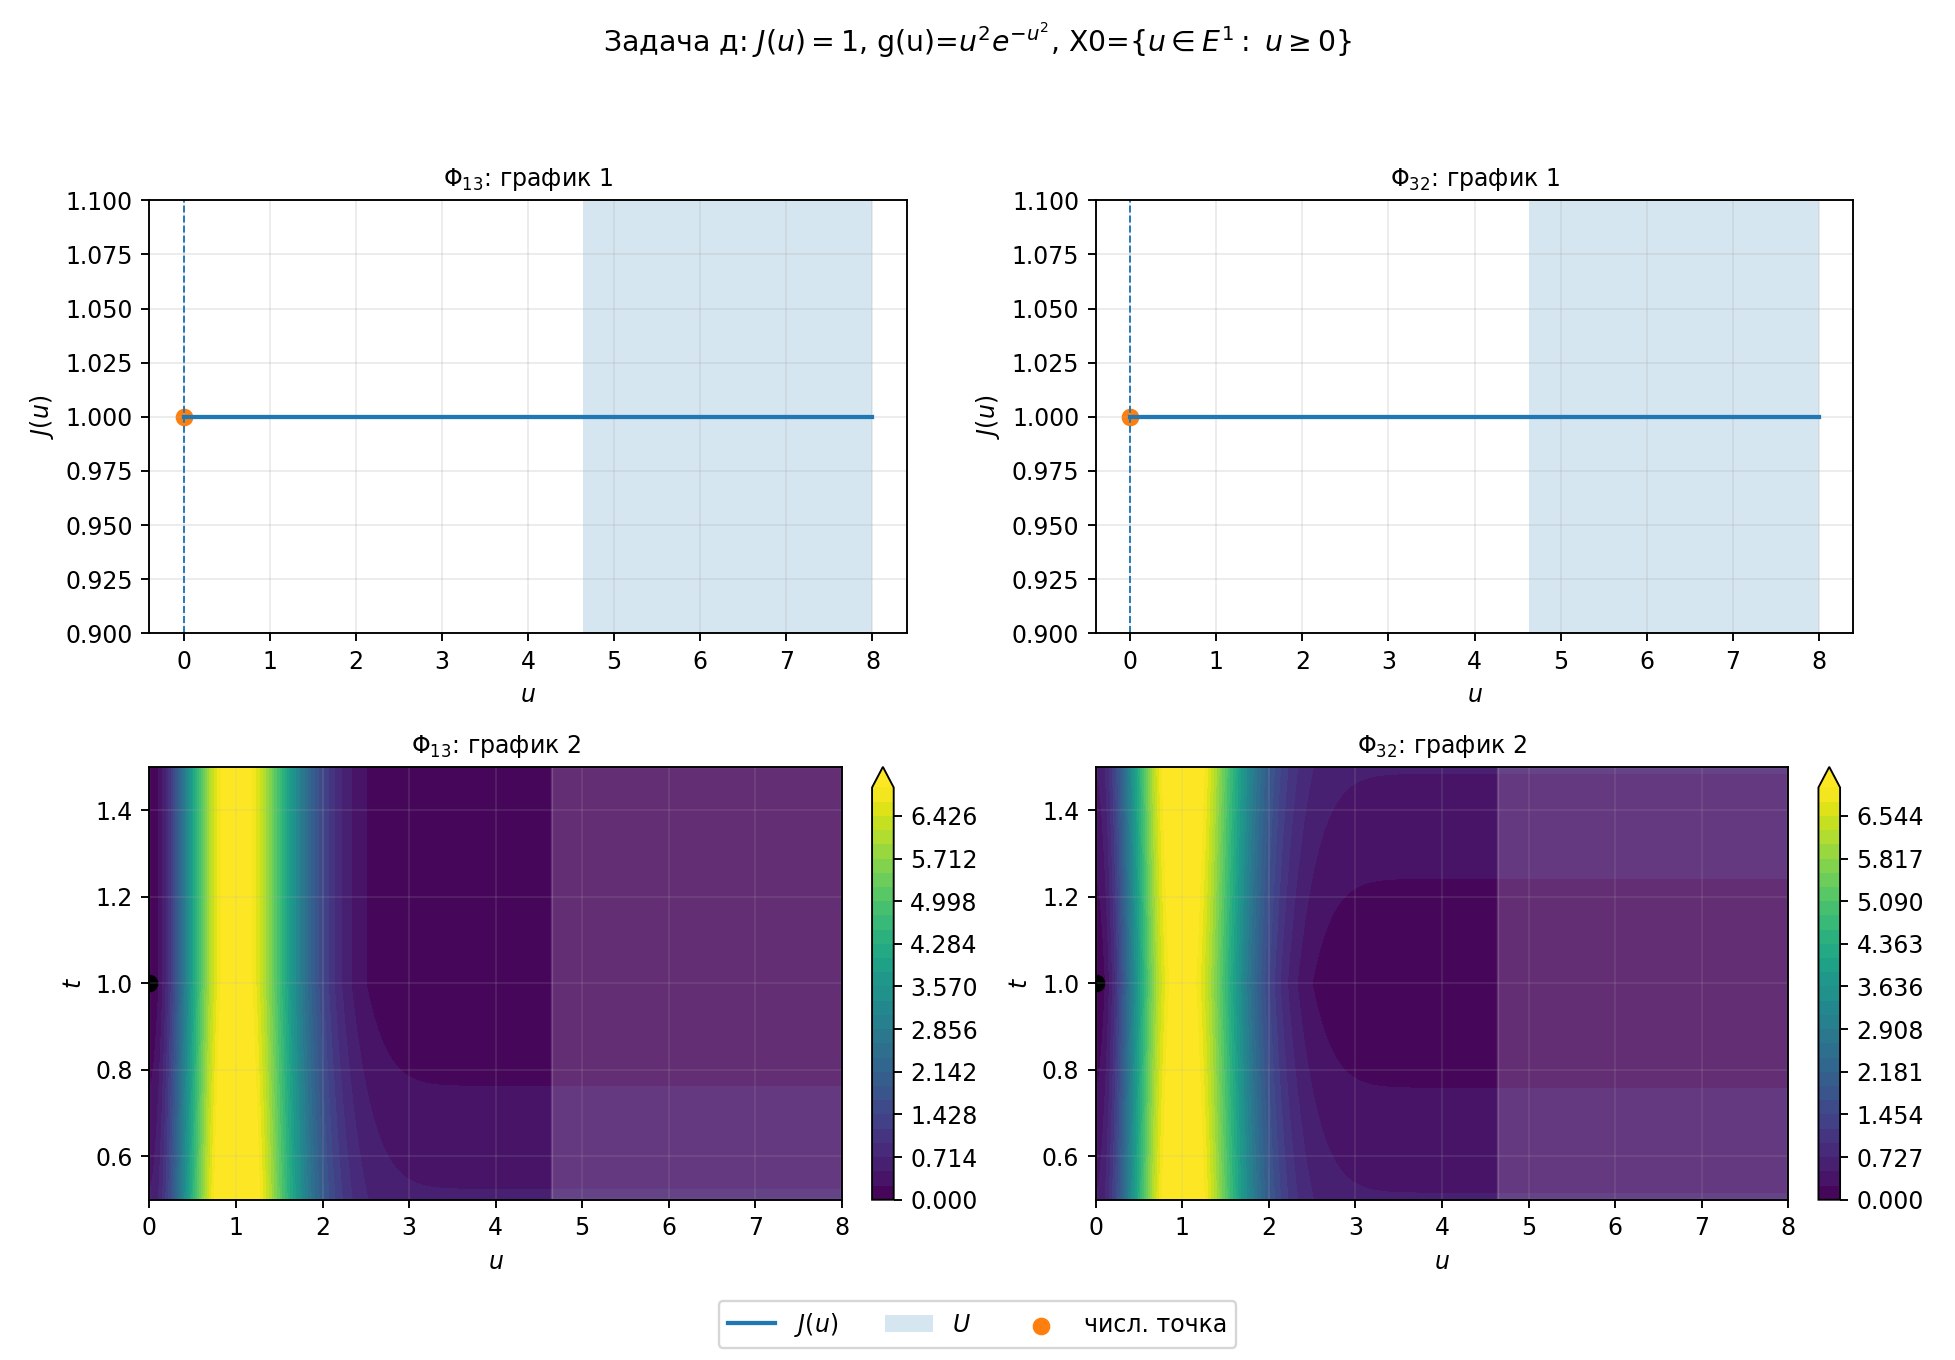
\includegraphics[width=0.96\textwidth]{graphs/d_g4_xge0_overview.png}
\caption{Задача д, вариант g4: $g(u)=u^2e^{-u^2}$, $X_0=\{u\in E^1:\ u\geq 0\}$. Верхний ряд: график 1 для $\Phi_{13}$ и $\Phi_{32}$; нижний ряд: график 2 для $\Phi_{13}$ и $\Phi_{32}$.}
\end{figure}


\section*{Вывод}
Исправленная реализация перебирает все варианты из упражнения, а не один выбранный вариант на пункт. Отдельная обработка \(U_0\) устраняет лишние ограничения при бесконечных концах области. В случаях, где выбранная функция \(g(u)\) задаёт пустое допустимое множество или нарушает согласованность постановки, это явно отражено в таблице: тогда условие \(t_*=J_*\) либо не проверяется, либо численный корень \(\rho(t)=0\) не совпадает с аналитическим инфимумом исходной задачи.

\end{document}
